\DIFdelbegin %DIFDELCMD < \chapter[On-line SNN training with SRM]{%%%
\DIFdelend \DIFaddbegin \chapter[On-line SNN Training with SRM]{\DIFaddend On-line SNN \DIFdelbegin \DIFdel{training }\DIFdelend \DIFaddbegin \DIFadd{Training }\DIFaddend with Spike-Based Rate Multiplication}
\label{cha:sdlm}
%Paragraph One: LINK
%Make a connection to what has immediately gone before. Recap the last chapter. In the last chapter I showed that… Having argued in the previous chapter that… As a result of x, which I established in the last chapter….. It is also possible to make a link between this chapter and the whole argument… The first step in answering my research question (repeat question) .. was to.. . In the last chapter I …
In the previous chapter we argued that deep Spiking Neural Networks~(SNNs) can be trained simply off-line on equivalent Artificial Neural Networks~(ANNs) and are equally capable of classifying hand written digits as are deep ANNs.
This chapter continues the discussion of the main research problem to narrow the gap of cognitive capabilities between spiking and conventional neural networks.
Instead of transforming off-line trained ANN models into SNNs, we explore on-line approaches which directly modulate the plastic synapses between spiking neurons in a biologically-plausible manner.
%The work of this chapter takes an extra step towards Neuromorphic Cognition, since the learning directly takes place on-line in SNNs.


%Paragraph Two: FOCUS
%Now focus the reader’s attention on what this chapter is specifically going to do and why it is important. In this chapter I will examine.. I will present… I will report … This is crucial in (aim of thesis/research question) in order to….
%In this chapter we present an on-line unsupervised learning algorithm, Spike-based Rate Multiplication~(SRM), working purely on event-based local STDP for training spiking Autoencoders and Restricted Boltzmann Machines.
%The SRM method represents the product of numerical values used in these unsupervised Deep Learning techniques with rate multiplication.
%The SRM then transforms the rate multiplication to the number of coincident spikes emitted from a pair of rate-coded spike trains, and the simultaneous events can be obtained by the biologically-plausible learning rule: Spike-Time-Dependant-Plasticity~(STDP).
%This on-line training method achieves better performance than existing algorithms and approaches the same, sometimes better performance of the equivalent non-spiking methods.
%It is crucial to provide deep SNNs with effective on-line training algorithms not only for building successful spike-based object recognition applications, but also for better power efficiency and scalability provided by the biologically-plausible SNN training on neuromorphic hardware.
\section{Introduction}
\label{sec:SRM_intro}
Before we investigate the proposed method, it is helpful to clarify what on-line learning addresses in the context of this thesis and what special features exist in SNN training.
Firstly, on-line systems `learn through play' in that there is no separation between a training and a testing phase.
Typically, the systems learn and improve their capability continuously as more data is fed into them.
Secondly, they `live and learn' which means on-line learning never stops.
Thus, it is easy for an on-line system to learn a \DIFaddbegin \DIFadd{new }\DIFaddend task, by simply providing different data.
However, once a model is trained off-line, it remains fixed and stops learning.
The brain is a natural on-line system, thus bringing its learning techniques to SNNs will equip neuromorphic computers with genuine learning capability, moving towards Neuromorphic Cognition.
Hence, thirdly, the on-line approach exploits biologically-plausible learning rules, e.g. Spike-Timing-Dependent Plasticity~(STDP).
Therefore, the modulation of the synaptic efficacy is event-driven by the spikes and operates in biological real time.

%Towards Neuromorphic Cognition, it is significant to endow these brain-like machines with on-line learning ability.

The main difficulty in proposing effective on-line methods is the lack of knowledge about learning in the brain.
The STDP learning rule, presented by~\citet{bi1998synaptic} (see Section~\ref{subsec:STDP} for detail), and its variations make up the majority of the biologically plausible on-line learning methods.
However, the most common training algorithm for an ANN, Backpropagation~(BP), is difficult to transform into STDP, since STDP \DIFdelbegin \DIFdel{only }\DIFdelend \DIFaddbegin \DIFadd{usually }\DIFaddend works locally with a teaching signal \DIFaddbegin \DIFadd{in supervised learning}\DIFaddend ; but, BP does not provide the teaching targets for all the hidden units of a network.
Therefore, existing on-line approaches, including our proposed method, favour greedy layer-wise unsupervised training in Deep Learning~\citep{hinton2006fast}.
\DIFaddbegin 

\DIFaddend Another problem is to \DIFdelbegin \DIFdel{accurately }\DIFdelend transform numerical calculations of weight changes into spike-based synaptic learning rules.
Existing methods suffer from performance loss due to imprecise translation.
\DIFdelbegin \DIFdel{Moreover, correlations between spike trains bring down the learning performance drastically after it peaks, thus making `live and learn' far from achievable in practice.
}%DIFDELCMD < 

%DIFDELCMD < %%%
\DIFdel{To address the problemof imprecise translation}\DIFdelend \DIFaddbegin \DIFadd{To address this problem}\DIFaddend , we propose the Spike-based Rate Multiplication~(SRM) method.
This algorithm \DIFdelbegin \DIFdel{is the first to transform }\DIFdelend \DIFaddbegin \DIFadd{transforms }\DIFaddend numerical calculations of weight tuning accurately into precise parameter configurations of equivalent STDP rules.
We select multiplication \DIFdelbegin \DIFdel{for translation into SNNs since }\DIFdelend \DIFaddbegin \DIFadd{to transform into SNNs for the reason that }\DIFaddend it is the core operation in the greedy layer-wise training of Autoencoders~(AEs\DIFdelbegin \DIFdel{, Equation~\ref{equ:ae_widrow_hoff}}\DIFdelend ) and Restricted Boltzmann Machines~(RBMs\DIFdelbegin \DIFdel{, Equation~\ref{equ:rbm_train}).
Regarding the performance loss caused by correlated spike trains, we put forward four methods to reduce the spike correlations while learning, which is the only attempt to tackle this problem as far as we know.
Therefore, the on-line learning can keep going without a continuous performance drop thanks to the proposed decorrelation methods. 
However, in the previous works, }\DIFdelend \DIFaddbegin \DIFadd{).
}

\DIFadd{Moreover, correlations between spike trains bring down the learning performance drastically after it peaks, thus }\DIFaddend the learning has to be manually stopped to avoid \DIFdelbegin \DIFdel{the performance loss.
The experimental result proves the precise translation of the SRM since the learning curves of the SNN experiments are well fitted to the non-spiking models;
in addition, the learning achieves the same, and sometimes even superior performance, as the conventional ANNs and stabilises around the peak performance without decay thanks to the decorrelation methods}\DIFdelend \DIFaddbegin \DIFadd{performance drop.
The problem makes `live and learn' far from achievable in practice.
%DIF > Thus, the learning has to be manually stopped to avoid performance loss.
Therefore, we put forward four methods to reduce the spike correlations while learning, thereby providing potential solutions to achieving genuine on-line learning on neuromorphic hardware}\DIFaddend .


%DIF > The experimental result proves the precise translation of the SRM, since the learning curves of the SNN experiments are well fitted to the non-spiking models;
%DIF > in addition, the learning achieves the same, and sometimes even superior performance, as the conventional ANNs and stabilises around the peak performance without decay thanks to the decorrelation methods.
\DIFaddbegin 








\DIFaddend %Paragraph Three: OVERVIEW
%The third paragraph simply outlines the way that you are going to achieve the aim spelled out in the previous paragraph. It’s really just a statement of the contents in the order that the reader will encounter them. It is important to state these not simply as topics, but actually how they build up the internal chapter argument… I will begin by examining the definitions of, then move to seeing how these were applied… I first of all explain my orientation to the research process, positioning myself as a critical scholar.. I then explain the methodology that I used in the research, arguing that ethnography was the most suitable approach to provide answers to the question of… 
%https://patthomson.net/2014/01/16/connecting-chapterschapter-introductions/

To begin with in Section~\ref{sec:SRM_related} we explore the research question of on-line, event-based deep SNN training in the literature.
In Section~\ref{sec:SRM} we describe SRM mathematically, and explain the factors influencing the accuracy of the method.
We then argue why the learning algorithm is suited to train spiking Autoencoders (SAEs) and Spiking Restricted Boltzmann Machines (SRBMs) in Section~\ref{sec:dSNN}.
During the research we encountered the problem of correlated spikes, and propose solutions to decorrelate spike trains in Section~\ref{sec:problem}.
Finally, experiments in Section~\ref{sec:SRM_result} show that this on-line training method achieves better performance than existing algorithms and approaches the same, sometimes superior performance of the equivalent non-spiking methods using detailed comparisons on the MNIST dataset.
%Finally, the online, spike-based learning algorithms demonstrate similar recognition and reconstruction capabilities to conventional DNN training on the detailed comparison on the MNIST dataset;



\section{Related Work}
\label{sec:SRM_related}
%To start with evidence of energy efficiency: maybe should refer to Chapter 2 or 1.
%The current trend towards training deep SNNs on-line using biologically-plausible learning methods is promising due to its potential benefit on low-energy hardware implementations.
%0. Dan Neil: Online Learning in Event-based Restricted Boltzmann Machines
The first on-line training algorithm \DIFdelbegin \DIFdel{for unsupervised learning }\DIFdelend \DIFaddbegin \DIFadd{using unsupervised Deep Learning }\DIFaddend was event-based Contrastive Divergence (evtCD)~\citep{neil2013online} for SRBMs, which established the feasibility of applying the STDP rule to an approximate CD algorithm.
A review of training methods for RBM algorithms is given in Section~\ref{sec:rbm}.
The evtCD method divided the learning process into potentiation and depression parts, which forms the basic design of related research.
Although it was also the first to intuitively transform numerical calculations to STDP rules, as an initial attempt mathematical estimation of the parameters was mainly ignored.
Therefore the best classification performance achieved was only about 81.5\% on the MNIST task, using purely spiking neurons.
%1. Neftci
\citet{neftci2013event} derived the division of potentiation and depression to their event-based CD algorithm, but conducted both parts on the same neural populations which was more biologically plausible.
Therefore, a global signal was needed to differentiate the potentiation and depression process.
The rhythmic oscillation of these processes generated a particular form of neural sampling~\citep{petrovici2013stochastic}.
The work focused on the statistical aspect of the event-driven sampling, and was extended to the later work on Synaptic Sampling Machines (S2Ms)~\citep{neftci2016stochastic} \DIFdelbegin \DIFdel{with }\DIFdelend \DIFaddbegin \DIFadd{using }\DIFaddend stochastic synapses.
The classification accuracy on MNIST was 91.9\%, 1.7\% lower than the conventional RBM\DIFaddbegin \DIFadd{, however was improved to 95.4}\% \DIFadd{by the S2M using the edge tool of Deep Learning: dropout~\mbox{%DIFAUXCMD
\citep{srivastava2014dropout}
}%DIFAUXCMD
}\DIFaddend .
Another similar work on SRBM training~\citep{burbank2015mirrored} applied the STDP rule to train SAEs in a very much biologically-plausible manner.
This work aimed at constructing artificial machine learning algorithms close to biology, whereas the other works above focused on training spiking Deep Learning modules with recognition capability\DIFdelbegin \DIFdel{equivalent to alternative Deep Learning methods}\DIFdelend .

%4. remote (ReSuMe)
The work we propose was mostly inspired by the supervised time-based spiking learning rule, ReSuMe~\citep{ponulak2010supervised}, where the output spikes of a post-synaptic neuron were trained to fire at the same times as the teaching spikes, see Figure~\ref{fig:resume}.
%So with certain input pattern injected to the pre-synaptic neurons, see Figure~\ref{fig:resume}.
The teaching signal always potentiates the synaptic strength while the output spikes of the post-synaptic neuron always depress the connection, and the weight change $\Delta w$ updates in accordance with the exponential STDP curve against the time difference between a \DIFdelbegin \DIFdel{post-synaptic spike }\DIFdelend \DIFaddbegin \DIFadd{post- }\DIFaddend and a pre-synaptic spike.
Therefore, as illustrated in Figure~\ref{fig:resume}, at the beginning the teaching spike fires earlier than the post-synaptic spike within an STDP window\DIFaddbegin \DIFadd{, $\tau_{win}$ }\DIFaddend which makes the weight potentiate more than it depresses;
thus \DIFaddbegin \DIFadd{(shown in the middle of Figure~\ref{fig:resume}) }\DIFaddend driven by a stronger synaptic weight, the post-synaptic neuron fires earlier than it is supposed to, making the weight depress a bit more than its potentiation;
finally, the weight stays unchanged because the post-synaptic neuron fires coincidently with the teaching spike, thus the weight's potentiation cancels out the depression.
\begin{figure}
	\centering
%	\begin{minipage}[c]{0.25\textwidth} 
%		\centering 
%		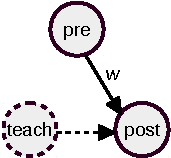
\includegraphics{pics_sdlm/ReSuMe.pdf} 
%	\end{minipage}
%	\begin{minipage}[c]{0.7\textwidth} 
%		\centering 
%		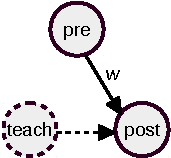
\includegraphics{pics_sdlm/resume.pdf} 
%	\end{minipage}
	\begin{subfigure}[c]{0.25\textwidth}
		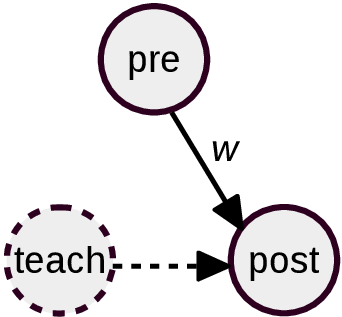
\includegraphics[width=\textwidth]{pics_sdlm/resume.png}
	\end{subfigure}
		\begin{subfigure}[c]{0.7\textwidth}
			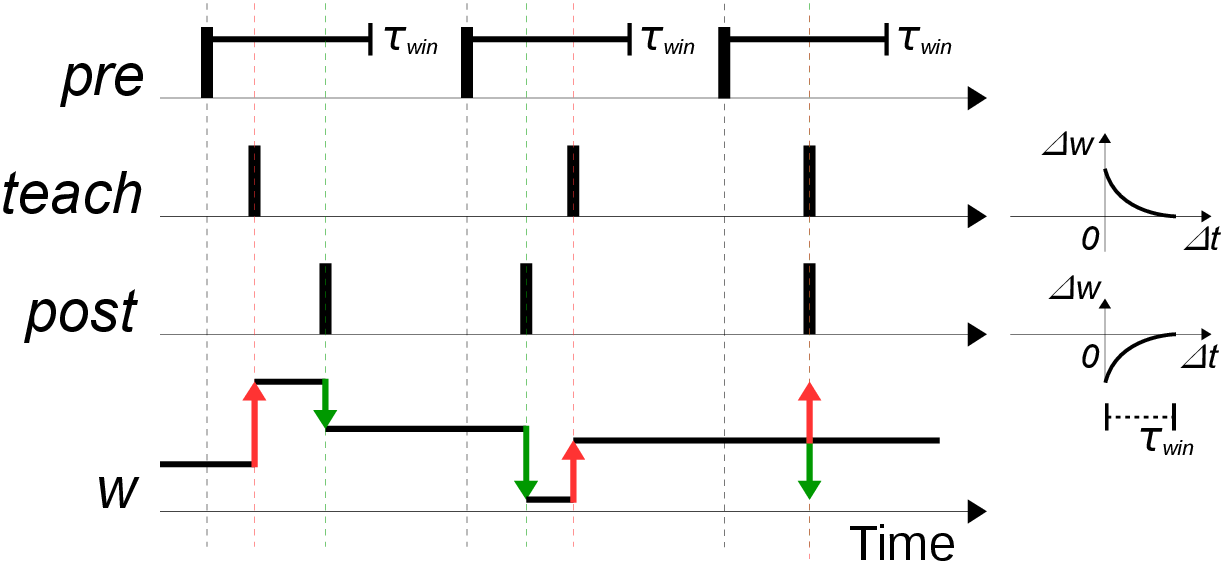
\includegraphics[width=\textwidth]{pics_sdlm/resume2.png}
		\end{subfigure}
	\caption[ReSuMe algorithm.]{A pair of pre- and post-synaptic neurons trained by ReSuMe~\citep{ponulak2010supervised} with a teaching signal.}
	\label{fig:resume}
\end{figure}

The inspiration of the proposed method is to provide a learning rule equivalent to ReSuMe on rate-encoded SNNs.
The objective is to cause the post-synaptic neuron to fire at the frequency of the teaching spike train. 
Accordingly, the weight decreases if the output neuron fires stronger than the teaching neuron, and vice versa.
The synaptic strength stops changing when the output neuron fires at the same frequency as the teaching signal.
In the following section, we will firstly describe this idea mathematically using the proposed term SRM, and equip the method with the ability to learn using a biological-plausible STDP rule.
%The algorithm is simply divided into spike-based rate multiplication (SRM) problems, and we will demonstrate the SRM method in following Section~\ref{sec:SRM}.
%The learning rule can be easily applied to SAEs if we use input spikes as teaching signals to the visible units, moreover the CD algorithm of training SRBMs is still not more than two operations of SRMs.
%Section~\ref{sec:dSNN} explains the specific training on SAEs and SRBMs in detail.


\section{Spike-based Rate Multiplication (SRM)}
\label{sec:SRM}
\begin{figure}
	\centering
%	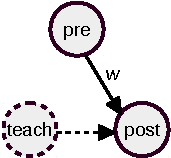
\includegraphics[width=0.3\textwidth]{pics_sdlm/resume.pdf}
	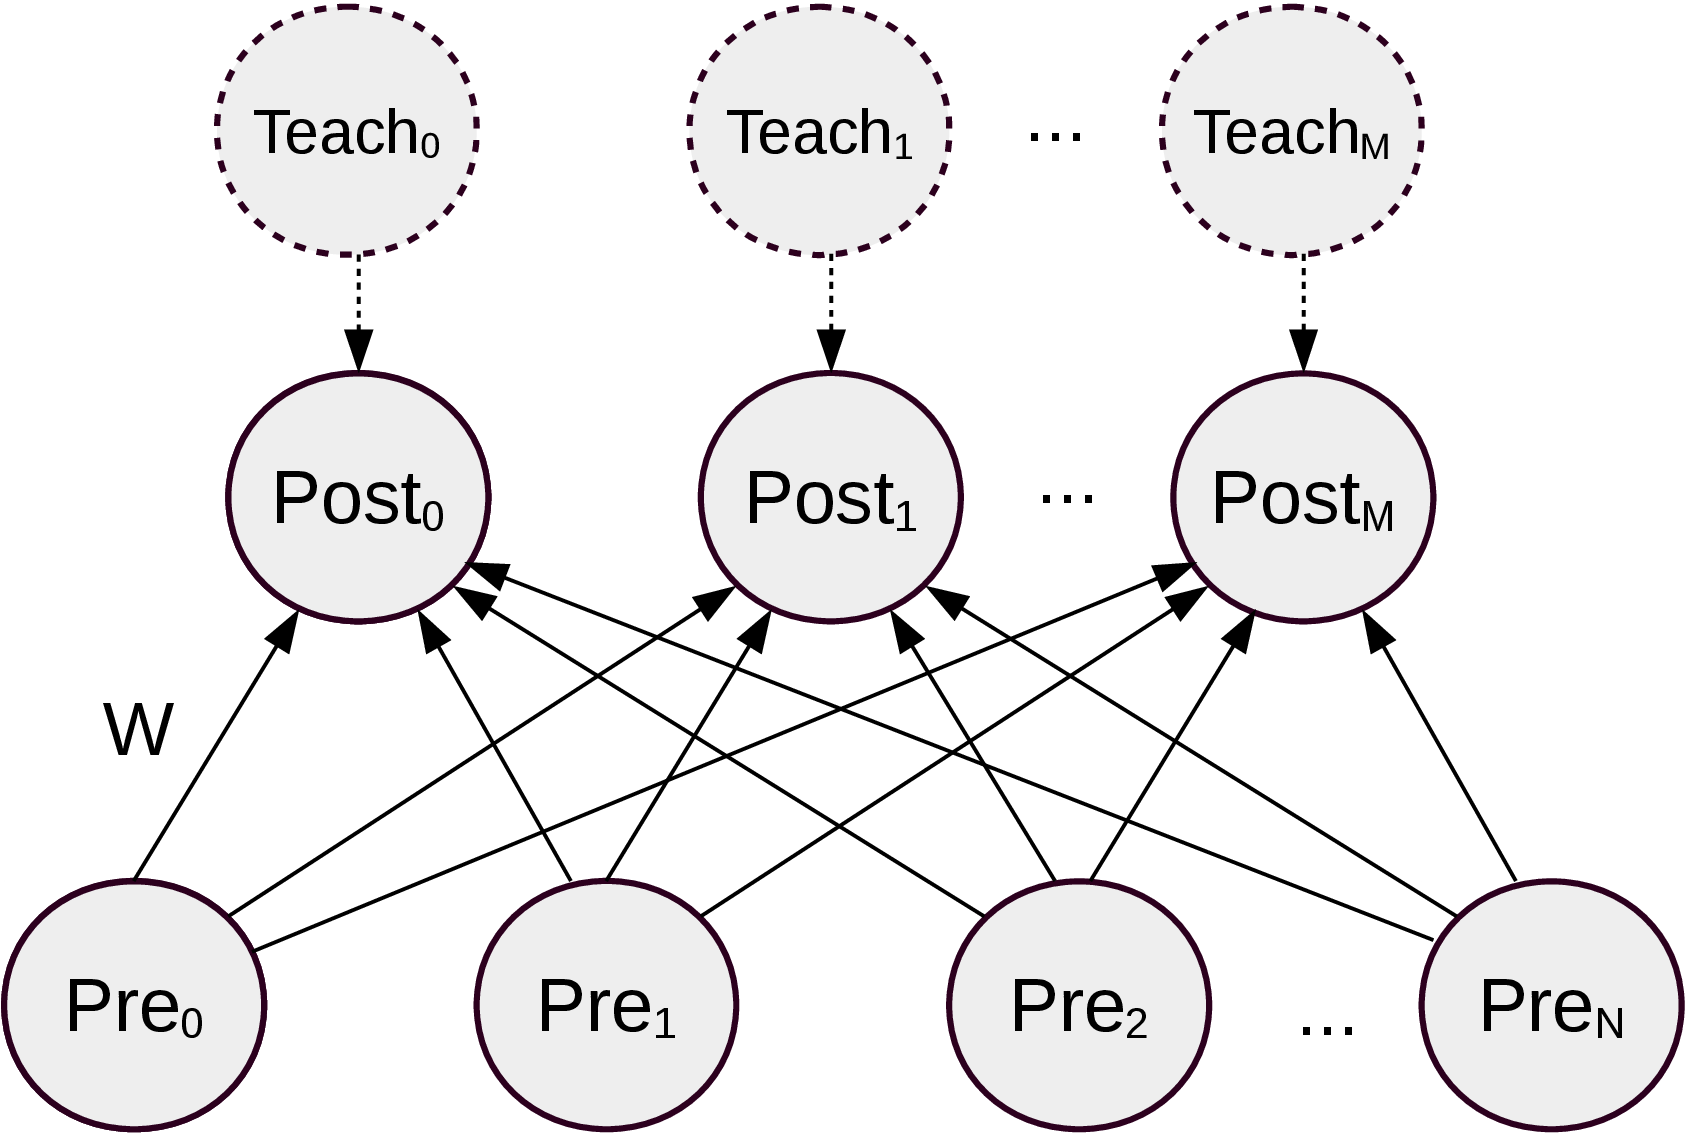
\includegraphics[width=0.6\textwidth]{pics_sdlm/adaline.png}
	\caption{The architecture of an ADALINE network.}
	\label{fig:adaline}
\end{figure}
Following the idea of reconstructing teaching signals in rate-based networks, we firstly look into existing models in ANNs.
If we see \textit{pre}, \textit{post} and \textit{teach} individually as vectors, and \textit{w} as a weight matrix of the all-to-all connections between \textit{pre} and \textit{post} in Figure~\ref{fig:resume}, it will form the ADALINE (Adaptive Linear Element)~\citep{widrow1960adaptive} network, see Figure~\ref{fig:adaline}.
The `Post' neurons perform a weighted sum on the input data, and the error between their output and the teaching data is propagated to update the weights, thus to train the network to generate the same output as the teacher. 
The learning algorithm was named Widrow-Hoff after the researchers:
\begin{equation}
\Delta w = \eta (teach - post)pre~.
\label{equ:widrow-hoff}
\end{equation}
%which is equivalent to Stochastic Gradient Descent~(SGD) in Multi-Layered Perceptrons~(MLPs).
The right hand side of the equation can be seen as a subtraction of two multiplication operations, $teach \times pre$ and $post \times pre$, times a learning rate, $\eta$.
Similarly, the unsupervised learning of AEs and RBMs has the same form of weight modulation, see Equations~\ref{equ:ae_widrow_hoff} and \ref{equ:rbm_train}:
\begin{equation}
\Delta w = \eta (ab-cd)~~.
\label{equ:two_sep}
\end{equation}
Especially for the training of AEs, the weight updates are the same as Equation~\ref{equ:widrow-hoff} if using the Rectified Linear Unit~(ReLU) as the activation function.

Therefore, multiplications are the core operations in the training of these rate-based ANN models.
Thus we propose the SRM accurately to transform the product of rates to weight tuning of event-based, biologically-plausible learning in SNNs.
There are a few steps to be followed: (1) \DIFdelbegin \DIFdel{present }\DIFdelend \DIFaddbegin \DIFadd{represent }\DIFaddend the rate multiplication with simultaneous spikes generated from a pair of connected spiking neurons;
(2) capture the simultaneous events in the weight change of the synaptic connection using the STDP learning rule.
(3) precisely transform the learning rate $\eta$ to parameters used in SRM.

\paragraph{1. Presenting rates with spikes\\}
%SRM provides the solution to present numeric multiplication $c=ab$ with rate-based spike trains.
Firstly, the multiplier $a$ and the multiplicand $b$ are encoded into Poisson spike trains $s_a(t)=\{s_a(1),s_a(2),...,s_a(T)\}$ and $s_b(t)=\{s_b(1),s_b(2),...,s_b(T)\}$ with 1~ms resolution, where $s(t)=1$ indicates a spike in the $t$th~ms and $s(t)=0$ means no spike.
Secondly, a Poisson generator fires a sequence of spikes according to its firing rate, $\lambda$~Hz, which is assigned linearly to the original multiplier/multiplicand \DIFdelbegin \DIFdel{by }\DIFdelend with a scaling factor of $K$.
Hence, the firing rate ($\lambda_x$) of the Poisson generator is $K$ times the numerical value x, and can be approximated by the average spike count, $N_T(s_x)$, of the generated spike train $s_x(t)$ over time $T$~ms:
\begin{equation}
\lambda_x = Kx \approx N_T(s_x) = \frac{1000}{T} \sum_{t=1}^{T} s_x(t)~,
\end{equation} 
1000 is the scale factor to transform frequency per millisecond to frequency per second.
Significantly, the approximation is more accurate as the observation time ($T$) grows since more spikes are generated over time and the average spike count becomes more reliable.
Thirdly, assuming $s_a(t)$ and $s_b(t)$ are independent Poisson spike trains the core definition of the rate multiplication of the pair of spike trains is as follows:
\begin{equation}
\lambda_a \lambda_b \approx N_{T_1}(s_a)N_{T_2}(s_b)= 10^6 \frac{\sum_{t_a=1}^{T_1}s_a(t_a)}{T_1}  \frac{\sum_{t_b=1}^{T_2} s_b(t_b)}{T_2}~.
\label{equ:mul}
\end{equation} 

%Finally, if we combine the concept of the STDP learning window with equation~\ref{equ:mul}, the length of the observing time on $s_b$ shrinks to a fixed-length windowing period, $\tau_{\textit{\textrm{win}}}$.
Finally, if we constrain the length of the observing time $T_2$ to a short time window $\tau_\textit{\textrm{win}}$ after each time step in $T_1$, the rate multiplication can be approximated with coincident spikes:
%The rate multiplication is then approximated by:
\begin{equation}
\lambda_a \lambda_b \approx \frac{10^6}{\tau_{\textit{\textrm{dur}}} \tau_{\textit{\textrm{win}}}} \sum_{t=1}^{\tau_{\textit{\textrm{dur}}}} [s_a(t) \sum_{t_b=t}^{t+\tau_{\textit{\textrm{win}}}} s_b(t_b)]~,
\end{equation} 
where $\tau_{\textit{\textrm{dur}}}$ replaces $T$ to represent the length of generated spike trains during SNN simulation.
Consequently, the rate multiplication can be conducted within only the local events in terms of time, although the accuracy may drop.
Here, we define the SRM function:
\begin{equation}
\begin{aligned}
\lambda_a \lambda_b \approx \textit{\textrm{SRM}}(s_a, s_b) 
%\tau_\textit{\textrm{dur}}, \tau_\textit{\textrm{win}}) 
= \frac{10^6}{\tau_{\textit{\textrm{dur}}} \tau_{\textit{\textrm{win}}}} \sum_{t=1}^{\tau_{\textit{\textrm{dur}}}} [s_a(t) \sum_{t_b=t}^{t+\tau_{\textit{\textrm{win}}}} s_b(t_b)]~.
\end{aligned}
\label{equ:srm_define}
\end{equation} 

\paragraph{2. Capturing coincident spikes with STDP.\\}
\begin{figure}
	\centering
	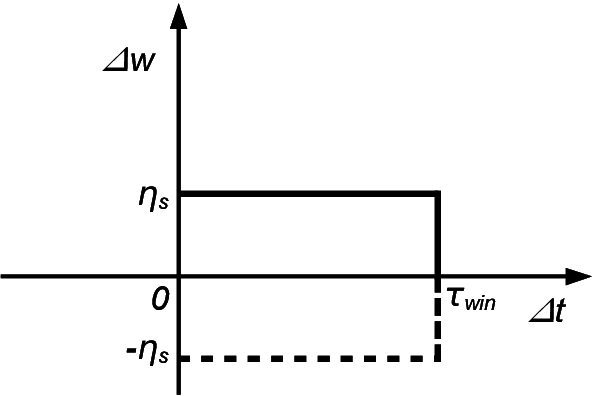
\includegraphics[width=0.4\textwidth]{pics_sdlm/stdp.png}
	\caption[Rectangular STDP curve.]{Rectangular STDP curve.
		If the time difference between the post-synaptic spike and the pre-synaptic spike lies in the window $\tau_{\textit{\textrm{win}}}$, then the synaptic weight will increase or decrease by $\eta_s$.}
	\label{fig:rtg_stdp}
\end{figure}
The weight rise/drop according to a rectangular STDP curve can detect the spike events of a pair of neurons when a post-synaptic spike occurs coincidently (within $\tau_{\textit{\textrm{win}}}$), see Figure~\ref{fig:rtg_stdp}:
\begin{equation}
\begin{aligned}
\Delta w &= \textit{\textrm{STDP}}(s_a, s_b)\\
% \tau_\textit{\textrm{dur}}, \tau_\textit{\textrm{win}}, \eta_s) 
&= \eta_s \sum_{t=1}^{\tau_{\textit{\textrm{dur}}}} [s_a(t) \sum_{t_b=t}^{t+\tau_{\textit{\textrm{win}}}} s_b(t_b)]~,
\end{aligned}
\end{equation}
where $ \eta_s$ represents the learning rate of the STDP rule.
Therefore, the overall weight change during time $\tau_{\textit{\textrm{dur}}}$ is determined by the number of coincident spikes of the pair of neurons, indicating the rate multiplication, and is described by SRM ( Equation~\ref{equ:srm_define}):
%Thus, SRM can be described with weight updates caused by STDP as defined in Equation~\ref{equ:srm_define}:
\begin{equation}
\begin{aligned}
\textit{\textrm{SRM}}(s_a, s_b) %, \tau_\textit{\textrm{dur}}, \tau_\textit{\textrm{win}})
&= \frac{10^6}{\tau_{\textit{\textrm{dur}}} \tau_{\textit{\textrm{win}}}} \sum_{t=1}^{\tau_{\textit{\textrm{dur}}}} [s_a(t) \sum_{t_b=t}^{t+\tau_{\textit{\textrm{win}}}} s_b(t_b)]\\
&= \frac{10^6}{\tau_{\textit{\textrm{dur}}}
\tau_{\textit{\textrm{win}}}
\eta_s}
\textit{\textrm{STDP}}(s_a, s_b)\\  %, \tau_\textit{\textrm{dur}}, \tau_\textit{\textrm{win}}, \eta_s) 
&= \frac{10^6}{\tau_{\textit{\textrm{dur}}}
\tau_{\textit{\textrm{win}}}
\eta_s}
\Delta w~~.
\end{aligned}
\end{equation}
%\begin{equation}
%\Delta w = \textit{\textrm{STDP}}(s_a, s_b, \tau_\textit{\textrm{dur}}, \tau_\textit{\textrm{win}}, \eta_s) = \eta_s \sum_{t=1}^{\tau_{\textit{\textrm{dur}}}} [s_a(t) \sum_{t_b=t}^{t+\tau_{\textit{\textrm{win}}}} s_b(t_b)]~,
%\end{equation}


\paragraph{3. Translating abstract numerical multiplication to SRM\\}
If we separate the weight updates of Equation~\ref{equ:two_sep} to a positive $\Delta w_+$ and a negative part $\Delta w_-$, the weight tuning can be described as:
\begin{equation}
\left\{
\begin{aligned} 
\Delta w_+ &= \eta ab\\
\Delta w_- &= -\eta cd
\end{aligned}
\right.~.
\end{equation}
Thus, it is straight forward to estimate the parameter $\eta_s$ to precisely transform the weight update from numerical calculations to spike-based learning rules:
\begin{equation}
\begin{aligned} 
\Delta w_+ = \eta ab &=\frac{\eta \lambda_a \lambda_b}{K^2}\\
&\approx \frac{\eta \textit{\textrm{SRM}}(s_a, s_b)}{K^2}\\ &=
\frac{\eta 10^6}{\tau_{\textit{\textrm{dur}}}
\tau_{\textit{\textrm{win}}}
\eta_s K^2}
\Delta w_+~,\\
\textrm{thereby,~~}
\eta_{s+} &=  \frac{\eta 10^6}{K^2 \tau_{\textit{\textrm{dur}}} \tau_{\textit{\textrm{win}}}}~,\\
\textrm{and similarly,~~}
\eta_{s-} &=  -\frac{\eta 10^6}{K^2 \tau_{\textit{\textrm{dur}}} \tau_{\textit{\textrm{win}}}}~.
%&\approx  \frac{10^6 SRM(s_a, s_b)}{K^2 \tau_{\textit{\textrm{dur}}} \tau_{\textit{\textrm{win}}}  \eta_s}~.
\end{aligned}
\label{equ:srm}
\end{equation}
So far we have accurately transformed numerical calculations of weight tuning to precise parameters of the SRM, thereby to the parameters of the STDP rules.


%We can adjust $\eta_s$ to $ K^2 \tau_{\textit{\textrm{dur}}} \tau_{\textit{\textrm{win}}}10^{-6}$ to make the numerical calculations to the spike-based presentations.
%In terms of the Widrow-Hoff learning algorithm:
%\begin{equation}
%	\eta_s=
%    \left\{
%    \begin{aligned} 
%    \eta K^2 \tau_{\textit{\textrm{dur}}} \tau_{\textit{\textrm{win}}}10^{-6}, &\text{ when calculating } \eta teach \times pre\\
%    - \eta K^2 \tau_{\textit{\textrm{dur}}} \tau_{\textit{\textrm{win}}}10^{-6}, &\text{ when calculating } \eta post \times pre
%    \end{aligned}
%    \right. ~.
%    \label{equ:eta_s}
%\end{equation}
%In Section~\ref{subsec:exp_AE}, we demonstrate how Widrow-Hoff algorithm successfully is applied to training AEs (see Equation~\ref{equ:ae_widrow_hoff}) and in Section~\ref{subsec:exp_SAE} we describe the implementation of SRM algorithm to Deep Learning models of spiking AEs and RBMs.

\paragraph{Last but not least, we state the property of the SRM algorithm:}
\begin{itemize}
	\item the accuracy of SRM is mainly controlled by $\tau_{\textit{\textrm{dur}}}$ and $\tau_{\textit{\textrm{win}}}$, where longer spike trains and a longer STDP window express the rate more reliably.
	\item in our spiking neural network both the multiplier and the multiplicand are presented only as rates, which are positive quantities.
	Thus a negative product is applied with weight decrease, $\eta_{s-}$. 
	\item the multiplier and the multiplicand are interchangeable due to the independence of the spike trains. 
	\item the accuracy is independent of the neural and synaptic models of the spiking neuron because the calculation relies only on the firing rate.
\end{itemize}


\section{Training Deep SNNs}
\label{sec:dSNN}
We have theoretically deduced the equivalence of the numerical weight update to the one-line spike-based STDP rules.
This section attempts to verify the SRM method in practice, thus we compare the learning performance of the conventional Deep Learning models to their spiking versions.
The experimental setup is described in Section~\ref{subsec:SNN_setup}, and the same experiments are carried out on all the training models for objective comparisons: AEs in Section~\ref{subsec:exp_AE}, RBMs in Section~\ref{subsec:exp_RBM}, SAEs in Section~\ref{subsec:exp_SAE} and SRBMs in Section~\ref{subsec:exp_SRBM}.
%The experimental result proves the precise translation of the SRM since the learning curves of the SNN examples are well fitted to the non-spiking models;

\subsection{Experimental Setup}
\label{subsec:SNN_setup}
\begin{figure}
	\centering
	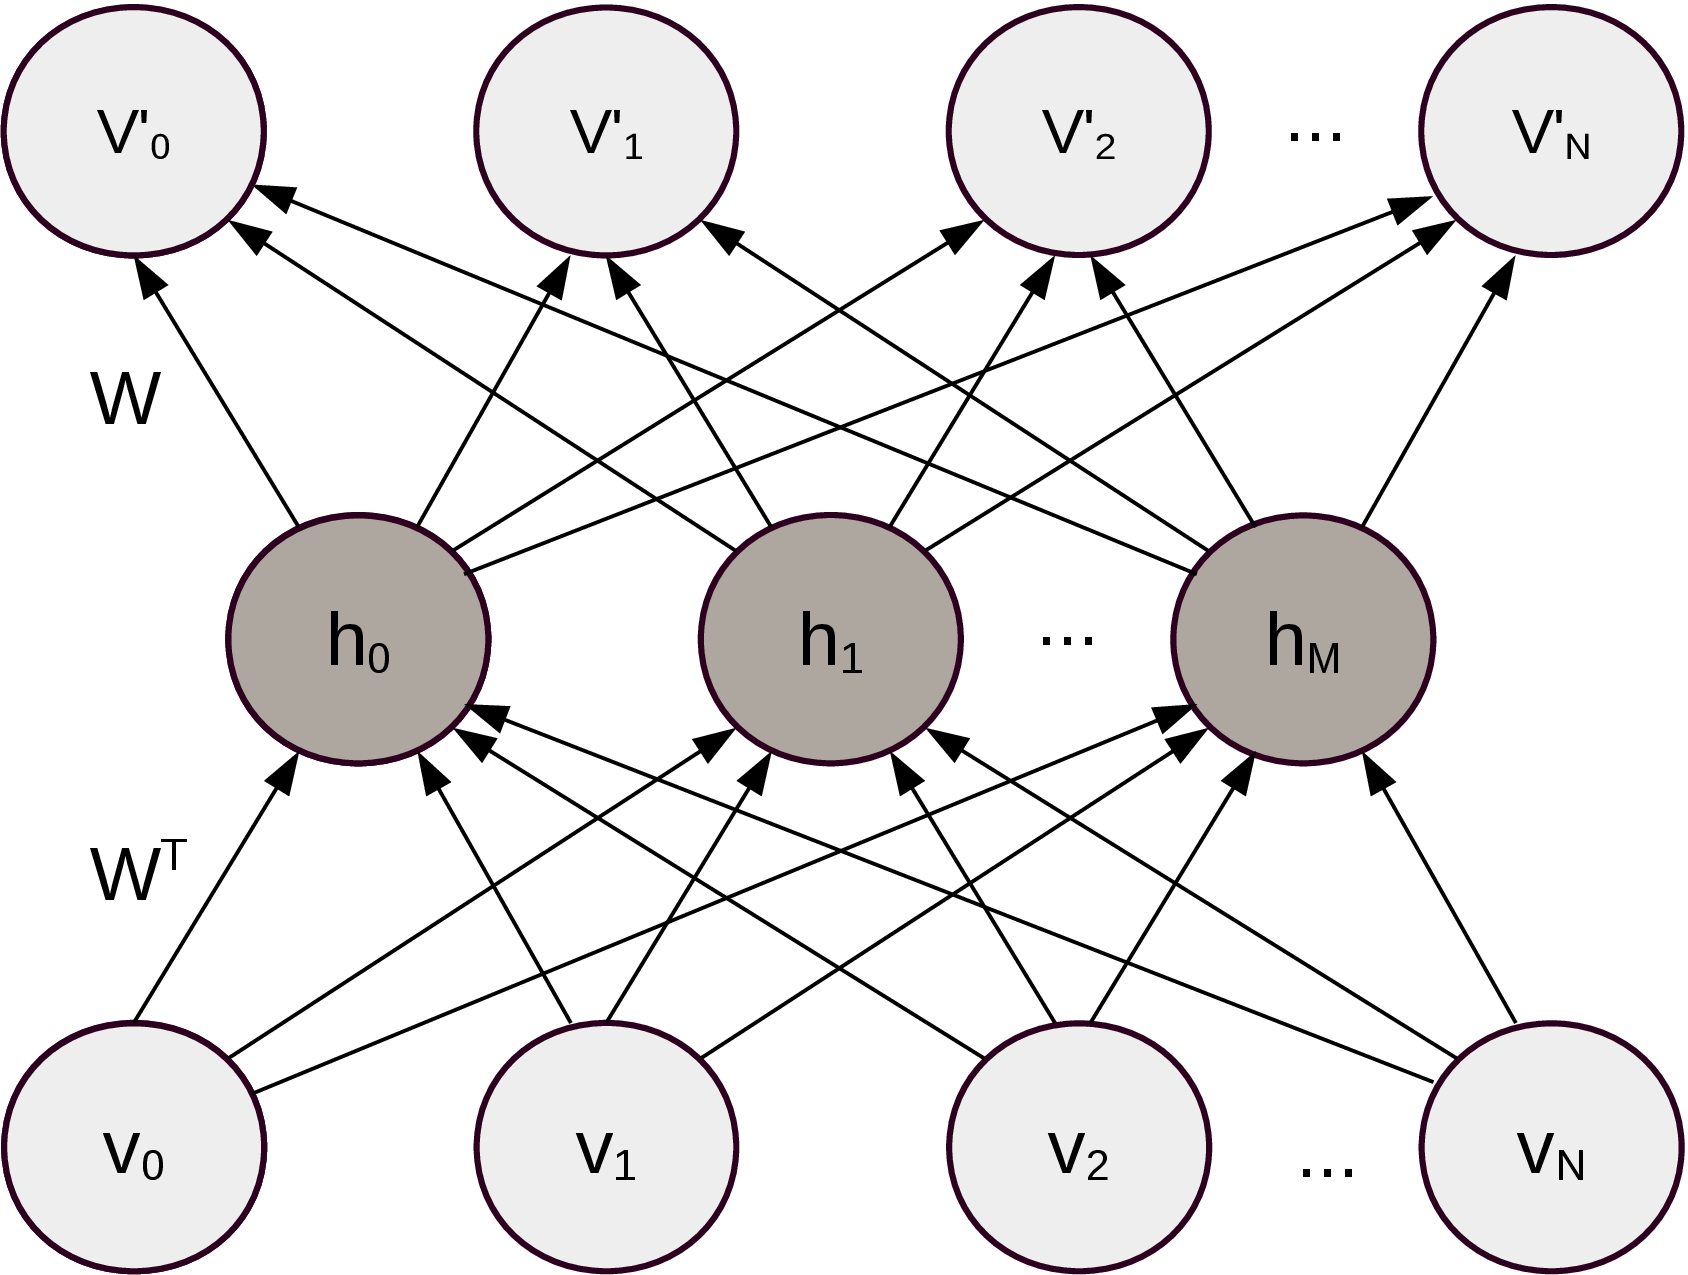
\includegraphics[width=0.5\textwidth]{pics_sdlm/AE.png}
	\caption[Reconstruction using AEs and RBMs.]{Symmetric weights connected between visible ($\bf{v}$) and hidden ($\bf{h}$) units in AEs and RBMs to reconstruct visible inputs, $\bf{v'}$.}
	\label{fig:sym_conn}
\end{figure}

There were two set-ups of the same network architecture~(Figure~\ref{fig:sym_conn}) where ten visible neurons connected to a layer of ten hidden neurons symmetrically with all-to-all weights: in Experiment~1 (Exp1), the values of all the input data were 1, $input_1 = [1, 1, 1,...,1]$; and in Experiment~2 (Exp2), the input data ranged from 0.1 to 1 linearly with steps of 0.1, $input_2 = [0.1, 0.2, 0.3,...,1]$.
These two experiments provided a close observation of the dynamic weight change given constant inputs.
Exp1 showed how the network responded to the same input value and reconstructed it, while Exp2 demonstrated the influence of ranging input values and, more importantly, how different firing rates may affect the corresponding SNN.
These experiments were run as baselines to compare with spike-based training on the features of weight convergence, reconstruction error and neural activities.


\begin{figure}
	\centering
	\begin{subfigure}[t]{0.48\textwidth}
		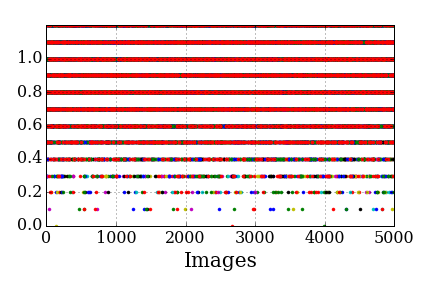
\includegraphics[width=\textwidth]{pics_sdlm/21_exp_AE_noise/exp1_input.png}
		\caption{Training input of Exp1}
	\end{subfigure}
	\begin{subfigure}[t]{0.48\textwidth}
		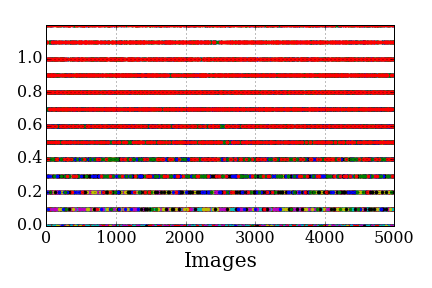
\includegraphics[width=\textwidth]{pics_sdlm/21_exp_AE_noise/exp2_input.png}
		\caption{Training input of Exp2}
	\end{subfigure}\\
	\begin{subfigure}[t]{0.48\textwidth}
		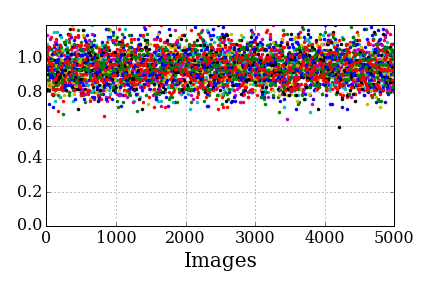
\includegraphics[width=\textwidth]{pics_sdlm/21_exp_AE_noise/exp1.png}
		\caption{Testing input of Exp1}
	\end{subfigure}
	\begin{subfigure}[t]{0.48\textwidth}
		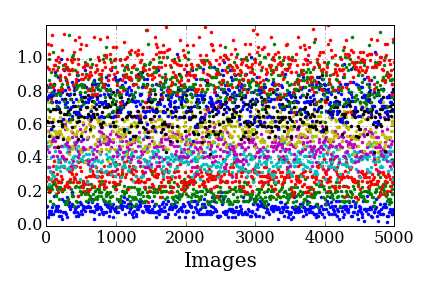
\includegraphics[width=\textwidth]{pics_sdlm/21_exp_AE_noise/exp2.png}
		\caption{Testing input of Exp2}
	\end{subfigure}
	\caption{Noisy input gathered from Poisson spike trains.}
	\label{fig:noise_input}
\end{figure}

The initial weights were randomly generated with unified distribution from 0 to 0.01 and the learning rate of conventional models $\eta$, was set to 0.001, and for spike-based training was set to 0.0001.
We kept the same initial weights for all the experiments thus providing an accurate comparison of the weight updates.
The input vector, seen as an image, repeatedly fed into the network $5,000$ times during training.
As a 'live and learn' system, there was no end to the learning, however for the purpose of observing the reconstruction performance, the weights were frozen every 10 steps of training and were validated on the testing data. 

Initially, AEs and RBMs were trained with clean numerical values, then with noisy values generated by counting the spikes in Poisson spike trains.
%presenting the original values with Poisson spike trains and transferring the spike counts back to numerical values.
The noisy data was gathered from the SNN experiments in Section~\ref{subsec:exp_SAE}.
%, and the corresponding SRM parameters were listed in Table~\ref{tbl:srm}.
All the SNN experiments used the same training and testing Poisson spike trains for the purpose of the unified experimental environment.

The firing rates of the input values were scaled up by the factor $K = 100$, thus $\lambda_1 = [100, 100, 100, ..., 100]$ Hz and $\lambda_2 = [10, 20, 30, ..., 100]$ Hz.
The spike count $N_{\tau_{\textit{\textrm{dur}}}}$ of the generated Poisson spike train then transformed to the noisy input\DIFaddbegin \DIFadd{~(NI) }\DIFaddend for use of conventional models: $N_{\tau_{\textit{\textrm{dur}}}}*1000/(\tau_{\textit{\textrm{dur}}} * K)$.
The scaling factor $1,000$ converts ms to s, and the length of spike trains $\tau_{\textit{\textrm{dur}}}$ was 100~ms when training, and $1,000$~ms for testing.
The longer the spike trains, the less noisy the spike counts become.
The \DIFdelbegin \DIFdel{noisy input }\DIFdelend \DIFaddbegin \DIFadd{NI }\DIFaddend can be seen as distorted data by adding Gaussian noise to the original value.
Hence, as shown in Figure~\ref{fig:noise_input}, the noisy training input added a Gaussian noise with -0.05 mean and 0.29 variance for Exp1 to the clean data, and -0.02 mean and 0.22 variance for Exp2;
while in terms of testing data, the means of the noise were the same, but the variances were much smaller: 0.09 for Exp1 and 0.07 for Exp2.


To compare all the following experiments, we present the results in the same template of figures:
among such a set of figures, (a) and (b) depict the weight changes of the two experiment set-ups (Exp1 and Exp2) which are the most important output of the training method;
(c) and (d) display the output of the visible units, the reconstruction of the input vector during testing;
(e) and (f) draw the output of the hidden units during testing and assist the observation of weight change and the reconstruction;
(g) and (h) intuitively show the loss (the mean squared error) and validate the accuracy of the reconstructions.

Following the experiments on conventional models, we propose the training methods for SAEs and SRBMs in detail.
The same experiments were then applied to the on-line and spike-based SNN training.

\DIFdelbegin %DIFDELCMD < \subsection{%%%
\DIFdel{Autoencoders (}\DIFdelend \DIFaddbegin \subsection[AEs]{\DIFadd{Training }\DIFaddend AEs\DIFdelbegin \DIFdel{)}\DIFdelend }
\label{subsec:exp_AE}
\begin{figure}
	\centering
	\begin{subfigure}[t]{0.48\textwidth}
		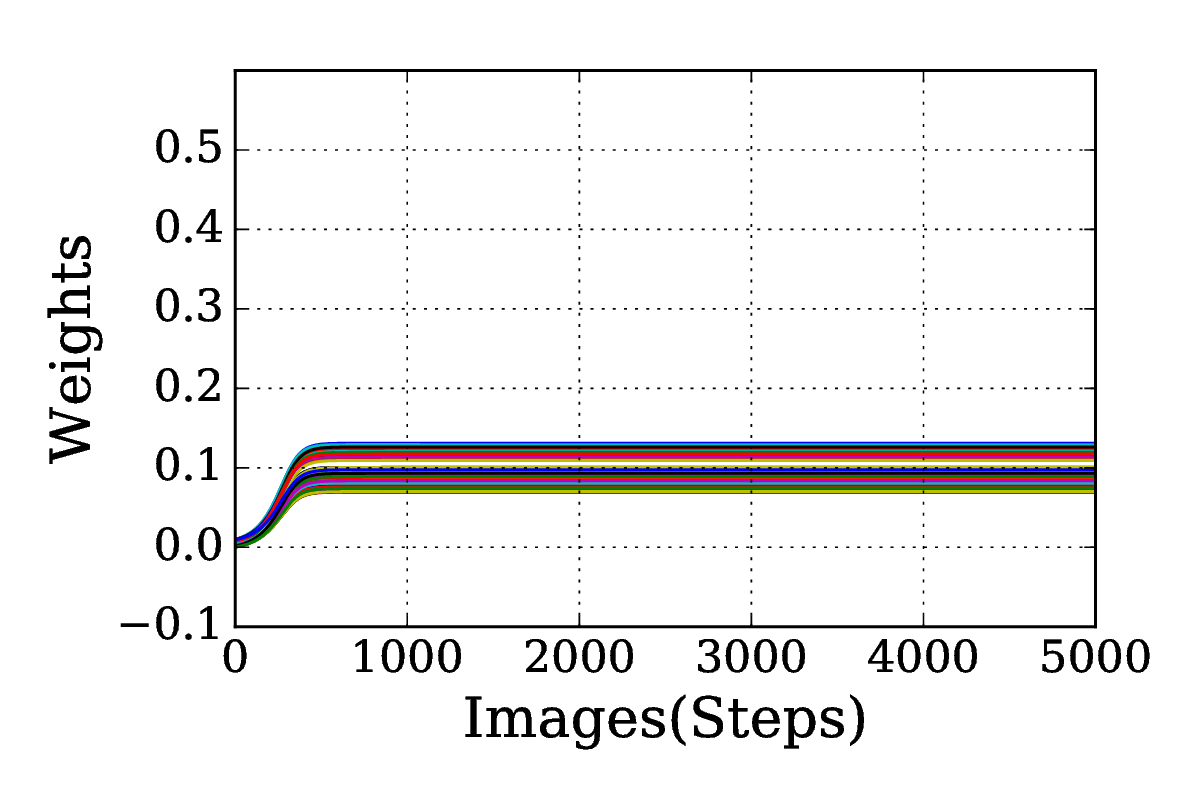
\includegraphics[width=\textwidth]{pics_sdlm/20_exp_AE/exp1_weights_non.png}
		\caption{Weights of Exp1}
	\end{subfigure}
	\begin{subfigure}[t]{0.48\textwidth}
		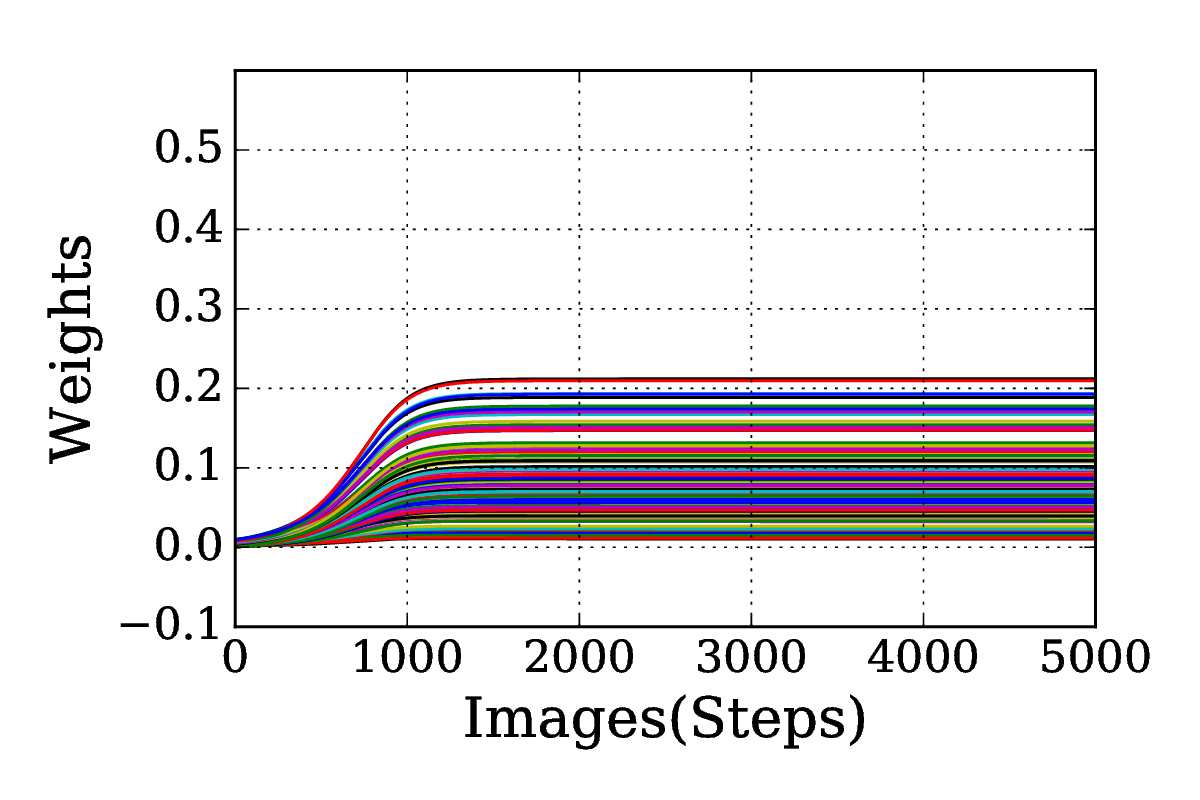
\includegraphics[width=\textwidth]{pics_sdlm/20_exp_AE/exp2_weights_non.png}
		\caption{Weights of Exp2}
	\end{subfigure}
	\begin{subfigure}[t]{0.48\textwidth}
		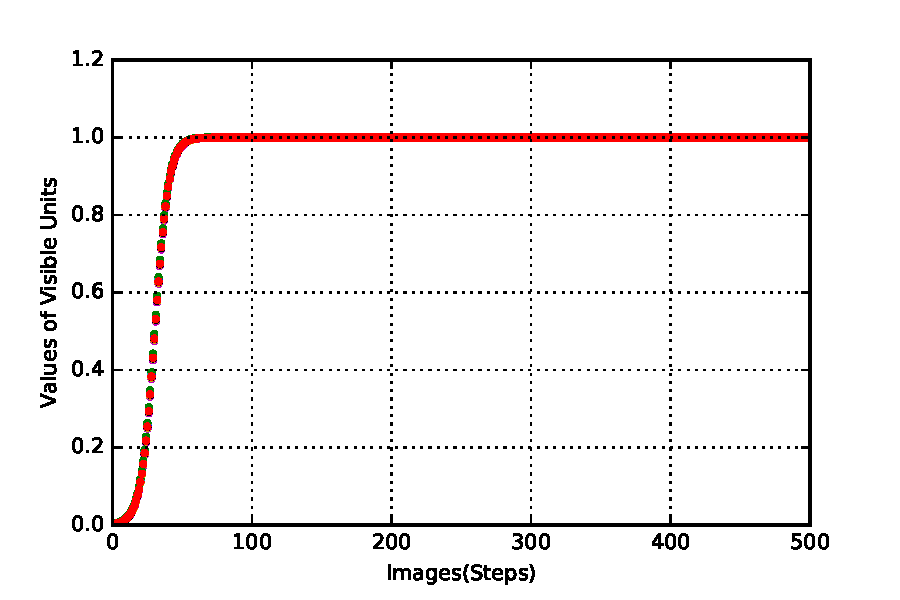
\includegraphics[width=\textwidth]{pics_sdlm/20_exp_AE/exp1_recon_non.pdf}
		\caption{Reconstruction of visible units in Exp1}
	\end{subfigure}
	\begin{subfigure}[t]{0.48\textwidth}
		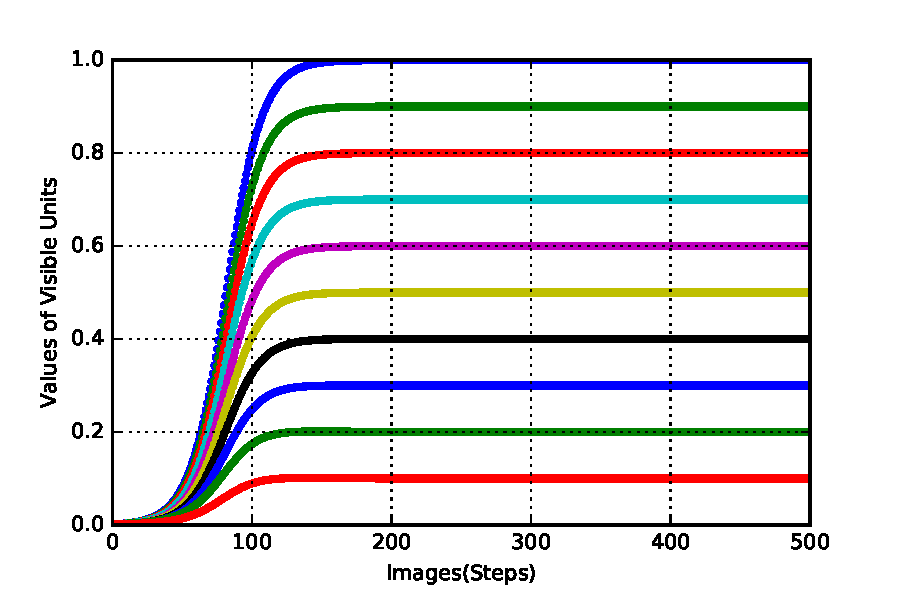
\includegraphics[width=\textwidth]{pics_sdlm/20_exp_AE/exp2_recon_non.pdf}
		\caption{Reconstruction of visible units in Exp2}
	\end{subfigure}\\
	\begin{subfigure}[t]{0.48\textwidth}
		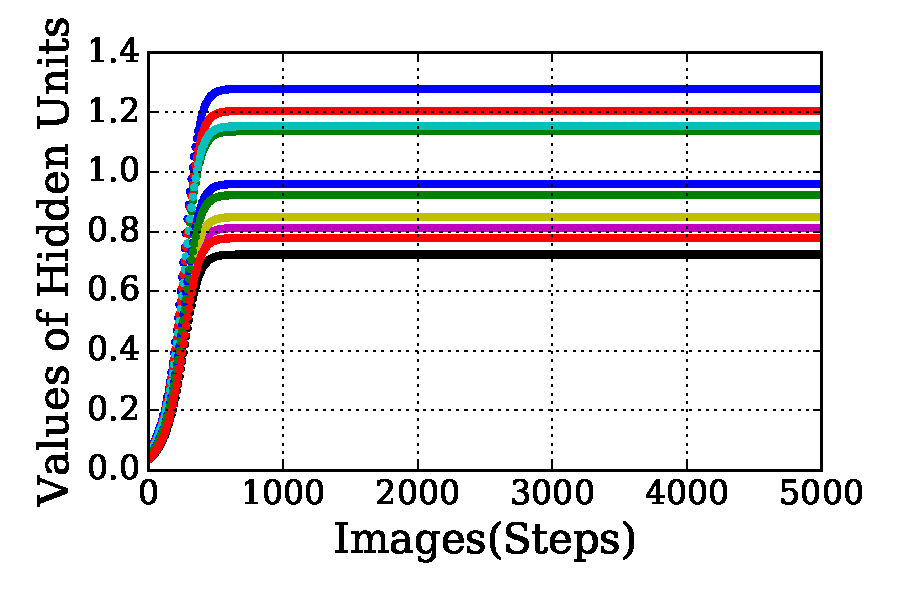
\includegraphics[width=\textwidth]{pics_sdlm/20_exp_AE/exp1_hid_non.pdf}
		\caption{Output of hidden units in Exp1}
	\end{subfigure}
	\begin{subfigure}[t]{0.48\textwidth}
		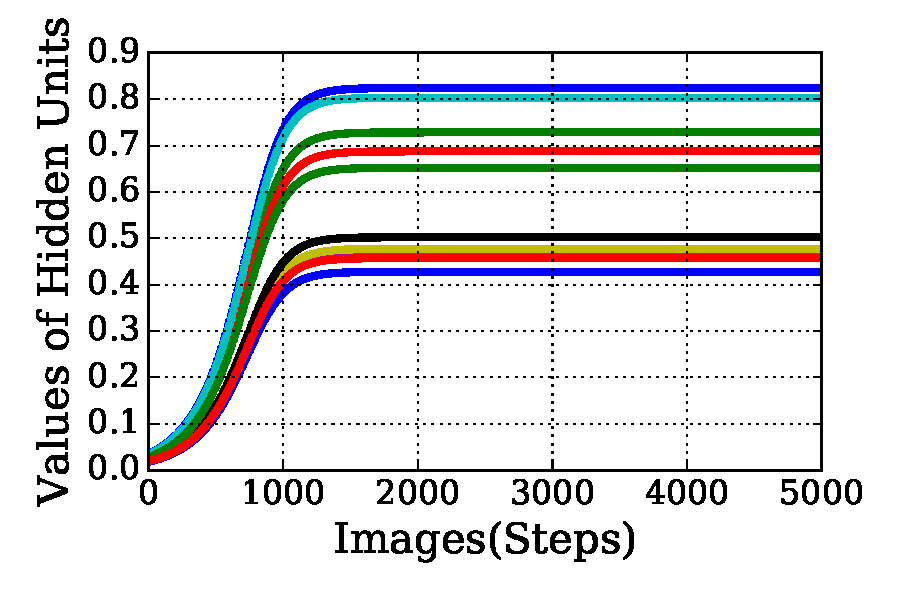
\includegraphics[width=\textwidth]{pics_sdlm/20_exp_AE/exp2_hid_non.pdf}
		\caption{Output of hidden units in Exp2}
	\end{subfigure}\\
	\begin{subfigure}[t]{0.48\textwidth}
		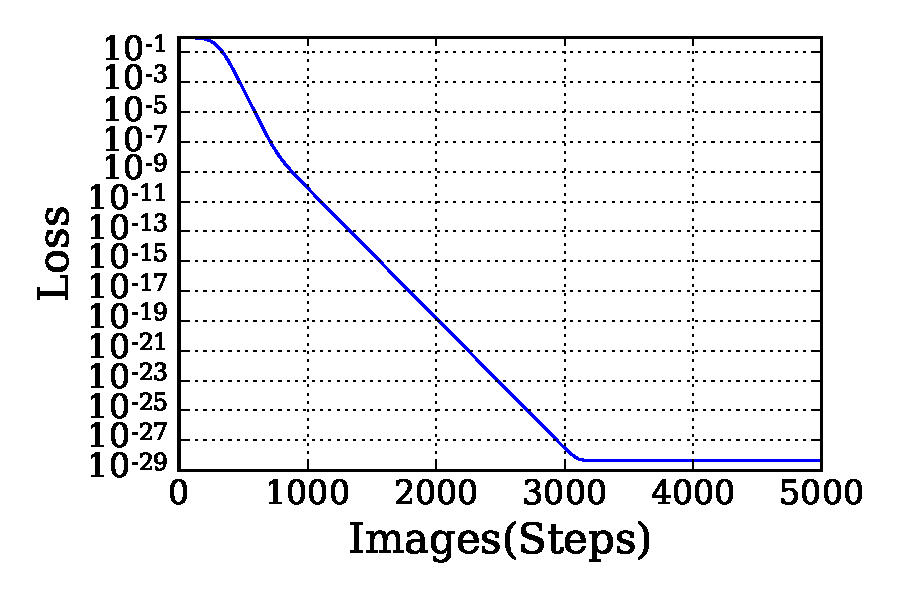
\includegraphics[width=\textwidth]{pics_sdlm/20_exp_AE/exp1_loss.pdf}
		\caption{Output of hidden units in Exp1}
	\end{subfigure}
	\begin{subfigure}[t]{0.48\textwidth}
		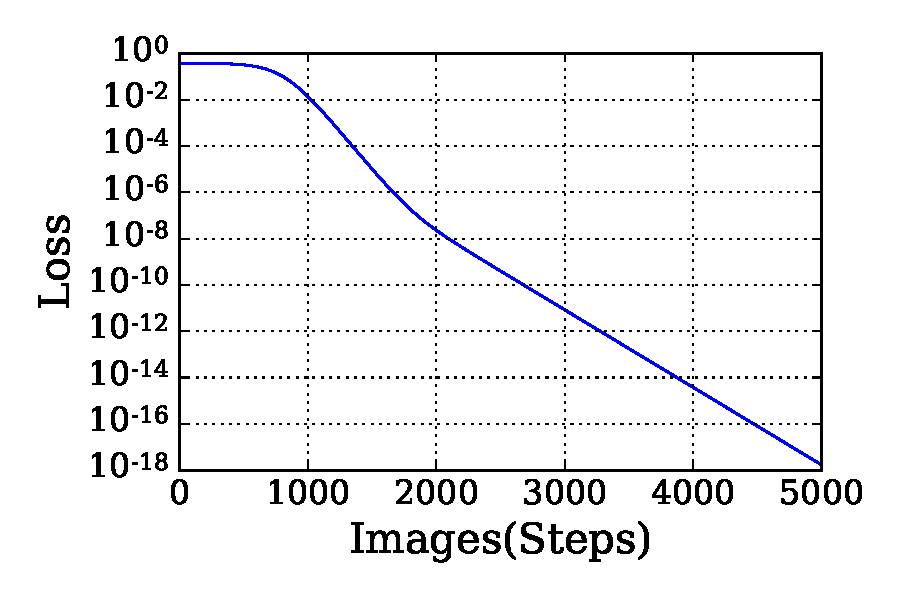
\includegraphics[width=\textwidth]{pics_sdlm/20_exp_AE/exp2_loss.pdf}
		\caption{Output of hidden units in Exp2}
	\end{subfigure}
	\caption[AE training of the reconstruction tests.]{Changes of weights, output of visible and hidden units, and mean squared error (loss) during the AE training of the reconstruction tests. 
		Experiments 1) 10 visible units fully connected to 10 hidden units with input data of all 1s; 2) the same network fed with 10 values distributed linearly from 0.1 to 1.}
	\label{fig:ae_orig}
\end{figure}
Using ReLU and Equation~\ref{equ:ae_widrow_hoff}, we can easily train a layer of AEs with such a small network.
For Exp1, Figure~\ref{fig:ae_orig} shows the dynamics of the AE as more repeating images are presented through training.
The reconstruction loss reduces exponentially to the limit of the computer's floating-point precision (Figure~\ref{fig:ae_orig}(g)), and reaches $10^{-4}$ using about 600 steps.
From that point the weights, visible reconstruction, and the output of the hidden units nearly stabilise, see Figure~\ref{fig:ae_orig}(a,c,e).
With the different input values of Exp2, the training runs slower, taking about $1,400$ steps to reach the same performance of $10^{-4}$ loss (Figure~\ref{fig:ae_orig}(h)).
The reason for the slower training is due to the weaker input which also results in lower output of the hidden units comparing to Exp1, see Figure~\ref{fig:ae_orig}(f), \DIFdelbegin \DIFdel{so that the positive part of the weight change, $\eta h_i v_j$, is much weaker}\DIFdelend \DIFaddbegin \DIFadd{thereby slowing down the weight increase}\DIFaddend . 
The reconstructions, shown in Figure~\ref{fig:ae_orig}(d), of smaller values stabilises earlier than those of higher values, since the higher output of the reconstruction requires stronger weights and more accumulated weight updates. 
\begin{figure}
	\centering
	\begin{subfigure}[t]{0.48\textwidth}
		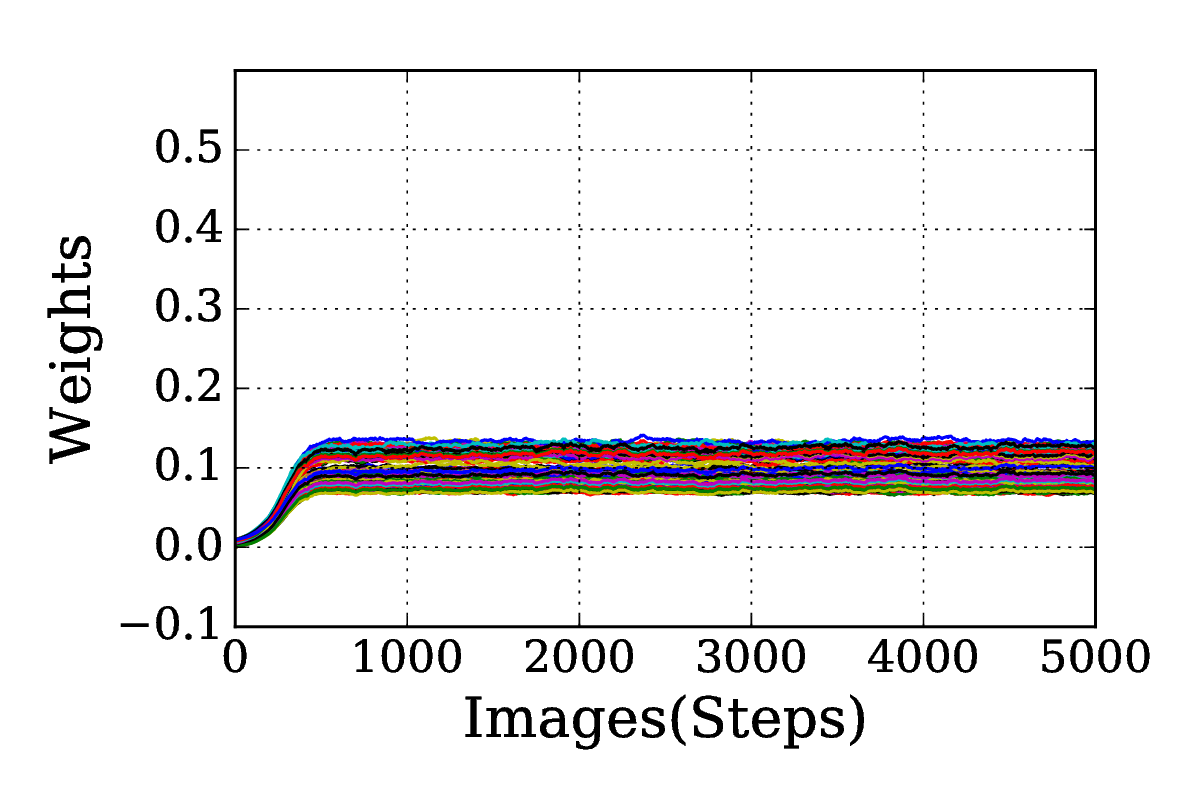
\includegraphics[width=\textwidth]{pics_sdlm/21_exp_AE_noise/exp1_weights_s.png}
		\caption{Weights of Exp1}
	\end{subfigure}
	\begin{subfigure}[t]{0.48\textwidth}
		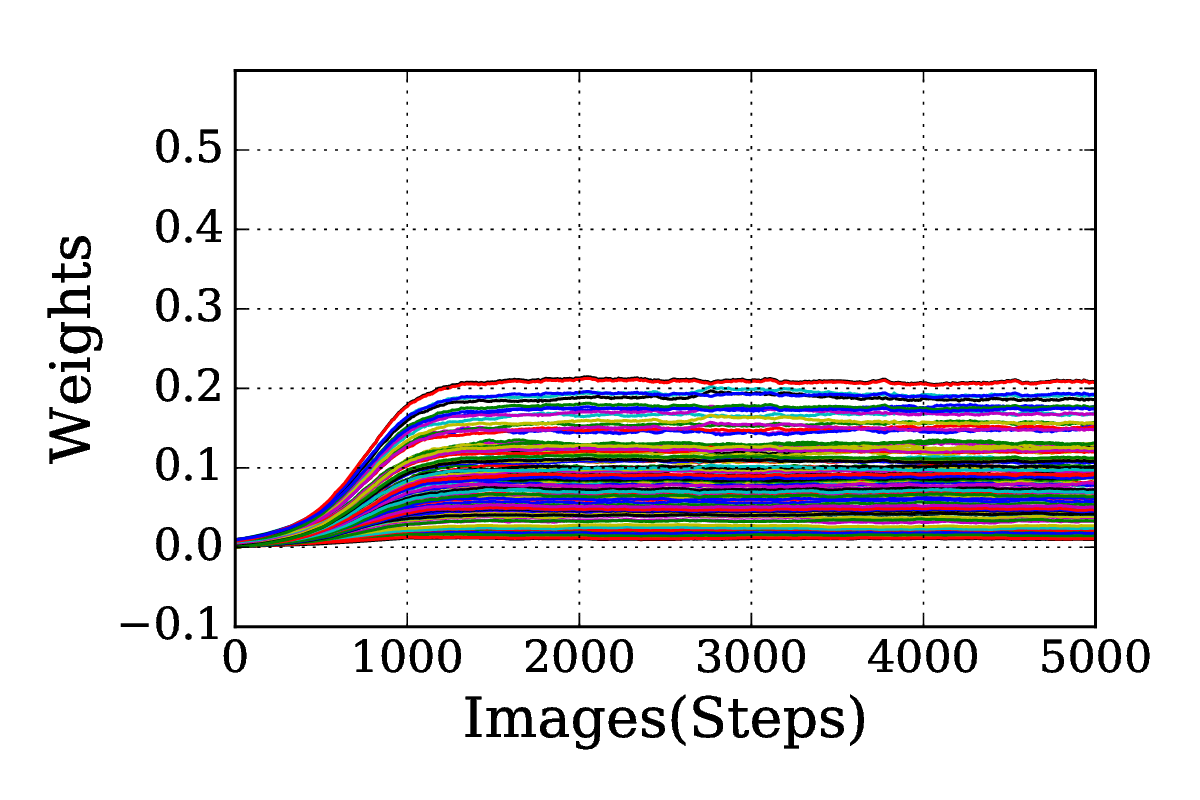
\includegraphics[width=\textwidth]{pics_sdlm/21_exp_AE_noise/exp2_weights_s.png}
		\caption{Weights of Exp2}
	\end{subfigure}
	\begin{subfigure}[t]{0.48\textwidth}
		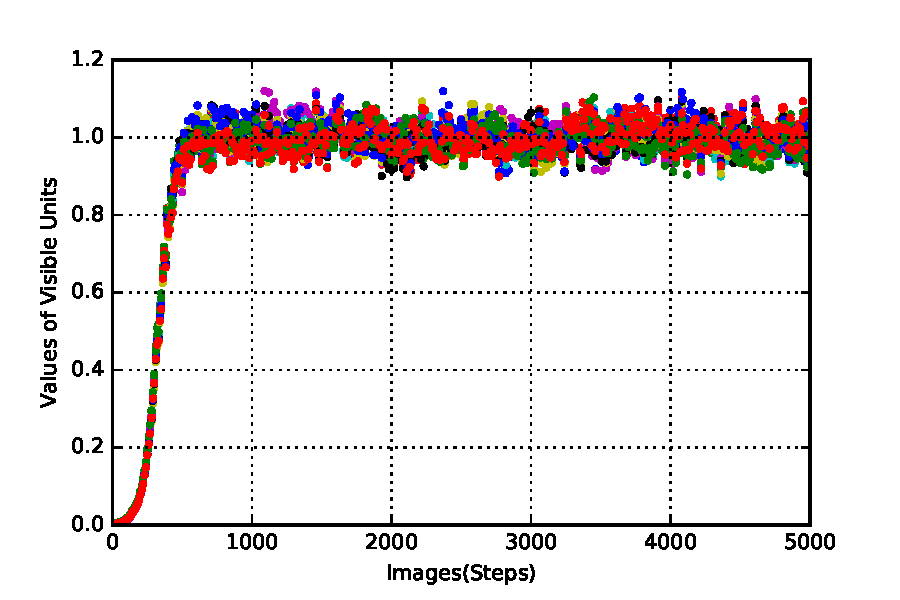
\includegraphics[width=\textwidth]{pics_sdlm/21_exp_AE_noise/exp1_recon_s.pdf}
		\caption{Reconstruction of visible units in Exp1}
	\end{subfigure}
	\begin{subfigure}[t]{0.48\textwidth}
		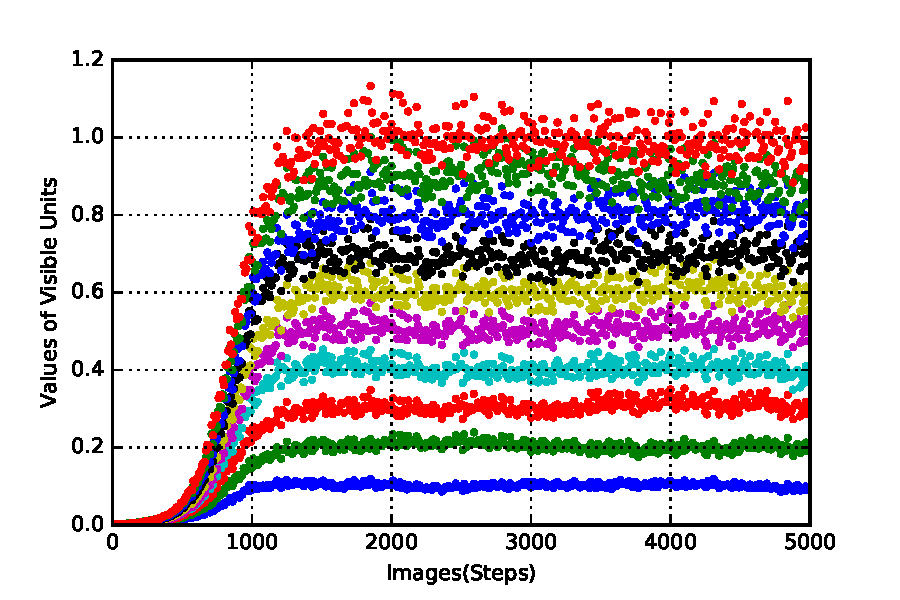
\includegraphics[width=\textwidth]{pics_sdlm/21_exp_AE_noise/exp2_recon_s.pdf}
		\caption{Reconstruction of visible units in Exp2}
	\end{subfigure}\\
	\begin{subfigure}[t]{0.48\textwidth}
		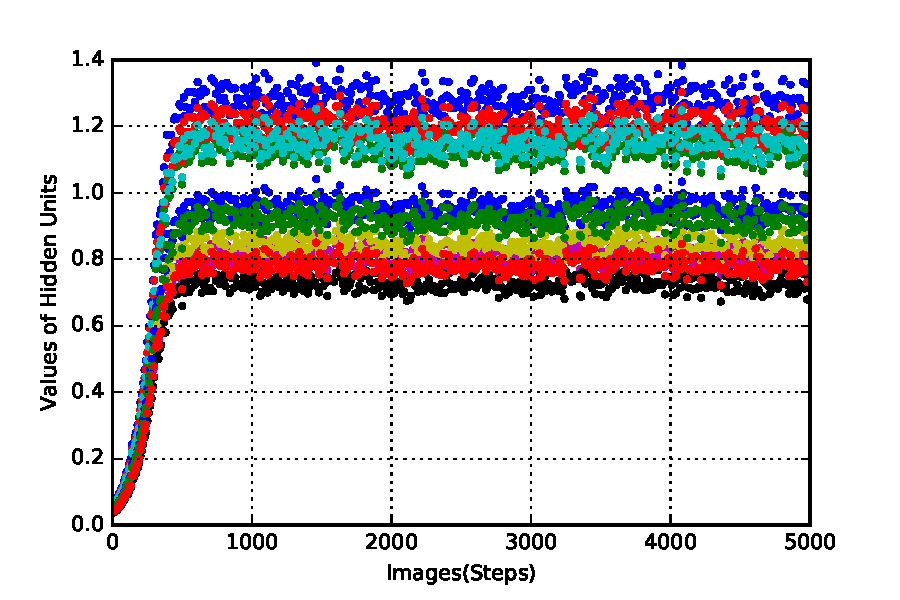
\includegraphics[width=\textwidth]{pics_sdlm/21_exp_AE_noise/exp1_hid_s.pdf}
		\caption{Output of hidden units in Exp1}
	\end{subfigure}
	\begin{subfigure}[t]{0.48\textwidth}
		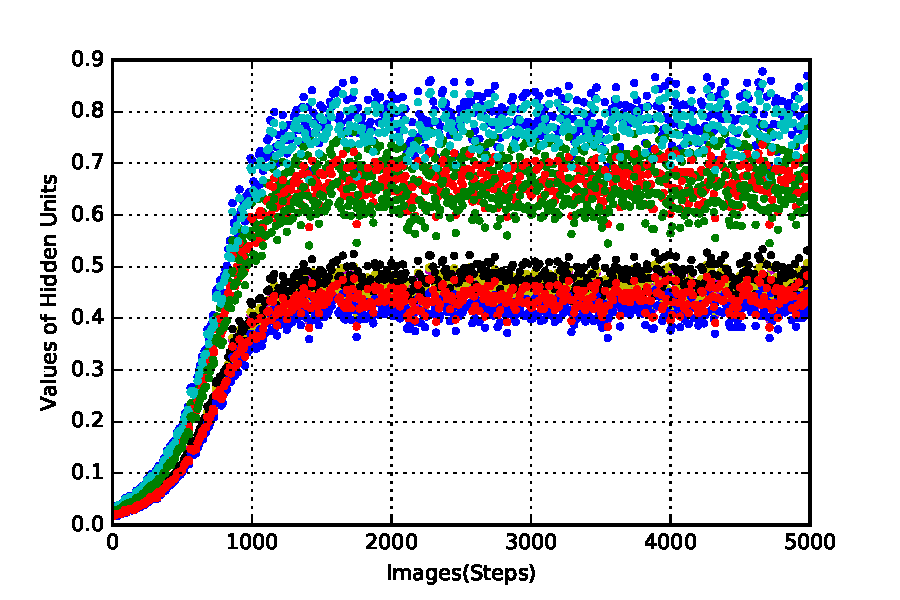
\includegraphics[width=\textwidth]{pics_sdlm/21_exp_AE_noise/exp2_hid_s.pdf}
		\caption{Output of hidden units in Exp2}
	\end{subfigure}\\
	\begin{subfigure}[t]{0.48\textwidth}
		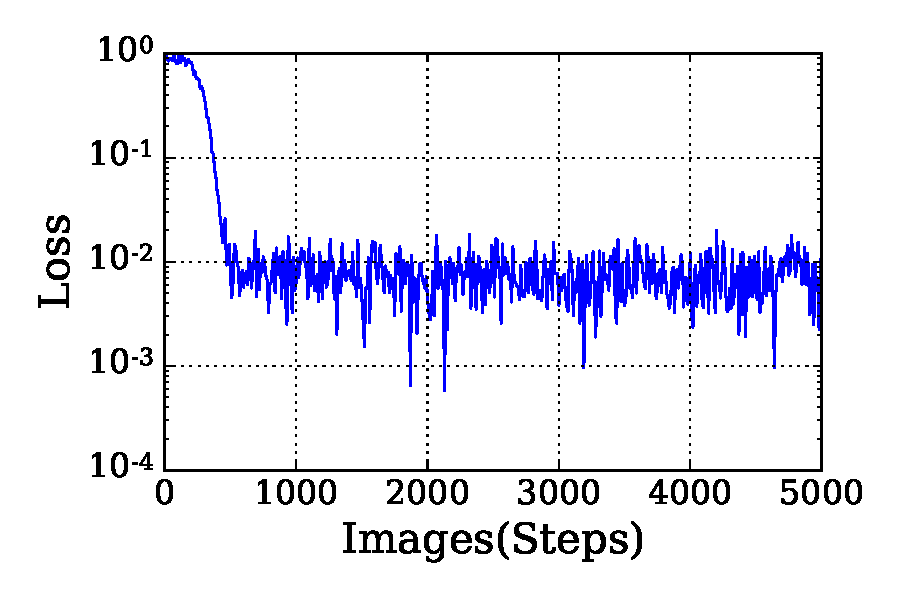
\includegraphics[width=\textwidth]{pics_sdlm/21_exp_AE_noise/exp1_loss_s.pdf}
		\caption{Output of hidden units in Exp1}
	\end{subfigure}
	\begin{subfigure}[t]{0.48\textwidth}
		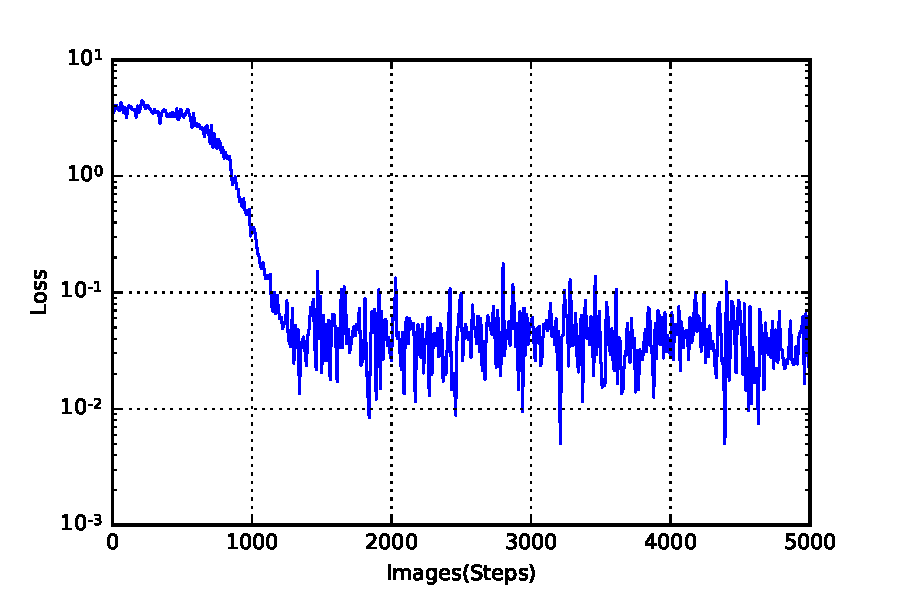
\includegraphics[width=\textwidth]{pics_sdlm/21_exp_AE_noise/exp2_loss_s.pdf}
		\caption{Output of hidden units in Exp2}
	\end{subfigure}
	\DIFdelbeginFL %DIFDELCMD < \caption[AE training of the reconstruction tests given noisy data.]{%%%
\DIFdelendFL \DIFaddbeginFL \caption[AE-NI training of the reconstruction tests.]{\DIFaddendFL Changes of weights, output of visible and hidden units, and mean squared error (loss) during the AE training of the noisy reconstruction tests. 
		Experiments 1) 10 visible units fully connected to 10 hidden units with the count of Poisson spikes firing at 100~Hz which lasted 100~ms; 2) the same network fed with spike count of Poisson spikes at firing rates ranging from 10~Hz to 100~Hz.}
	\label{fig:ae_noise}
\end{figure}

The same experiments were repeated with noisy training and test data to provide a fair comparison with the spike-based Deep Learning modules.
Figure~\ref{fig:ae_noise} shows the effect of the \DIFdelbegin \DIFdel{noisy input}\DIFdelend \DIFaddbegin \DIFadd{NI}\DIFaddend , although the training stabilises at roughly the same time point.
Firstly, it generates slight fluctuations in the weight change.
Secondly, the reconstruction and the output of the hidden units are noisy compared to those of clean data.
However, the noise is much reduced from the \DIFdelbegin \DIFdel{noisy input }\DIFdelend \DIFaddbegin \DIFadd{NI }\DIFaddend data compared to Figures~\ref{fig:noise_input}~(c) and (d), indicating the robustness of AEs. 
Finally, the losses keep at a certain level and stops dropping.
The loss in Exp2 is lower than Exp1, in other words the reconstruction on Exp2 is closer to the input data.
This is mainly caused by the weaker noise level on the smaller input values which makes the data of Exp2 less noisy on average.
So is the reconstruction, which leads to the lower level of loss.
\begin{figure}
	\centering
	\begin{subfigure}[t]{0.48\textwidth}
		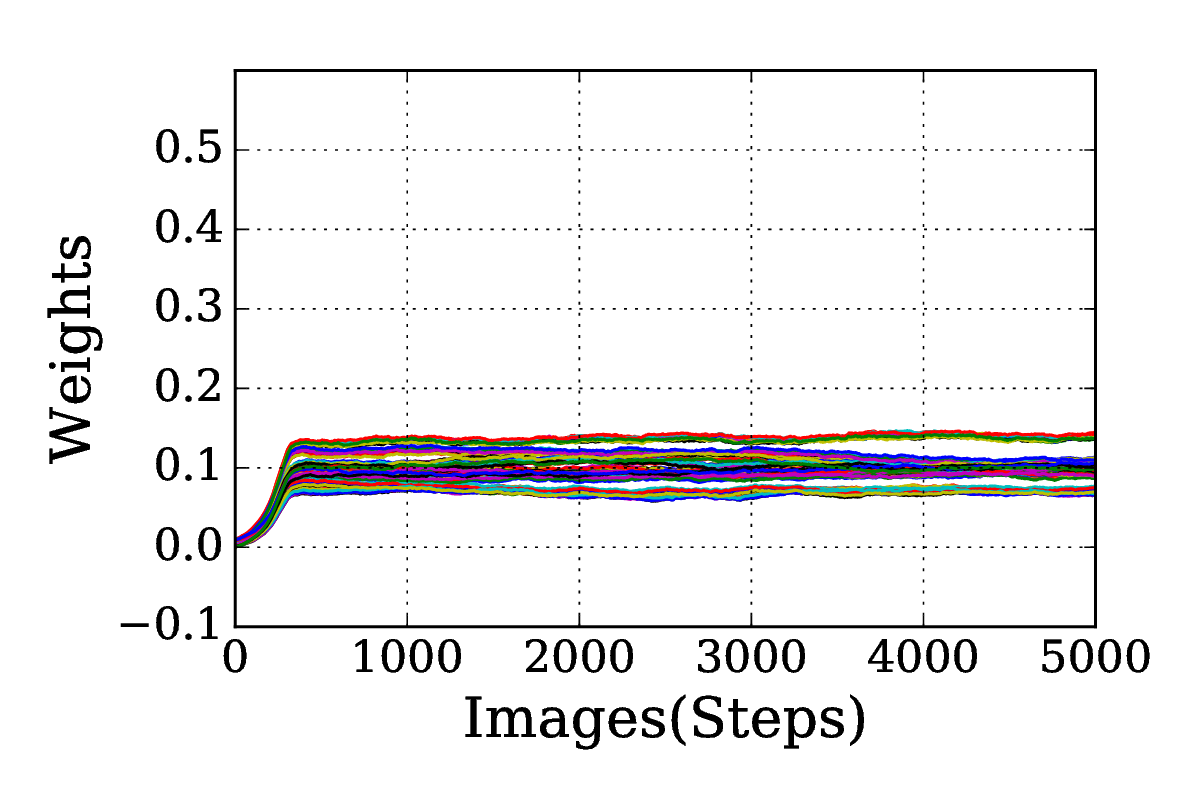
\includegraphics[width=\textwidth]{pics_sdlm/30_exp_RBM/exp1_weights_non.png}
		\caption{Weights of Exp1}
	\end{subfigure}
	\begin{subfigure}[t]{0.48\textwidth}
		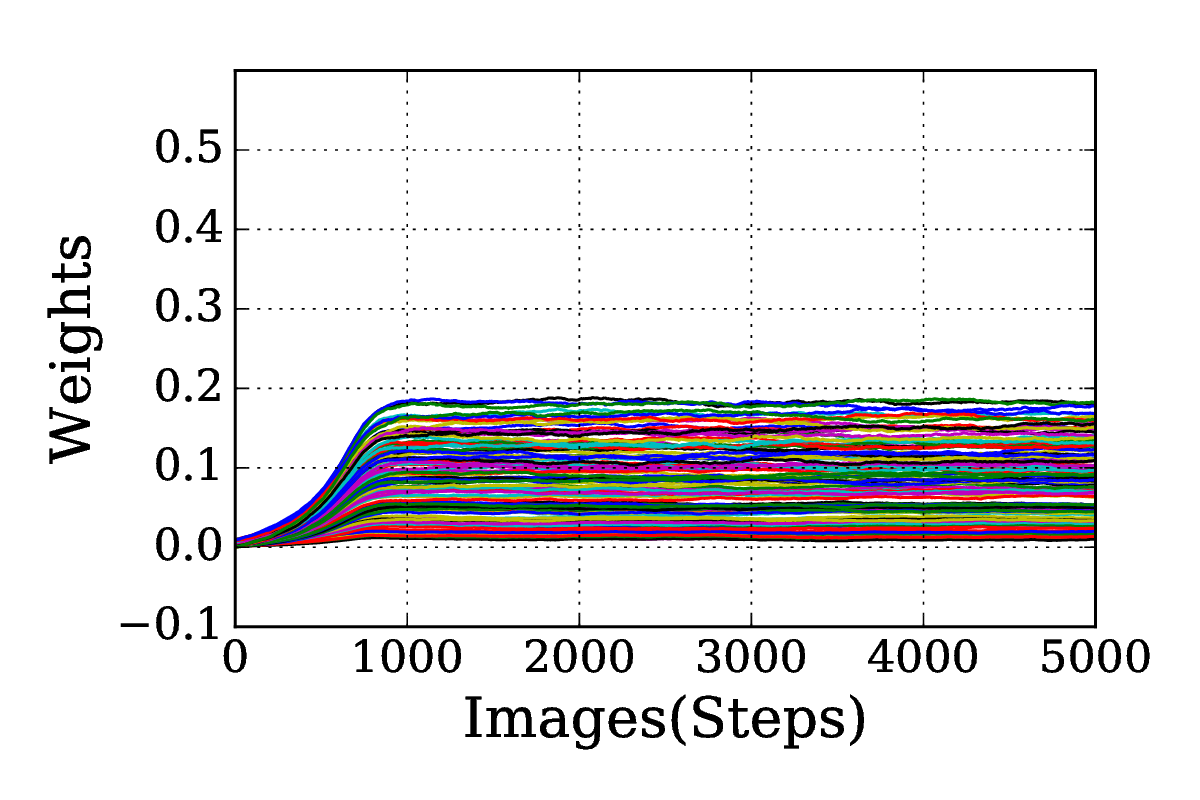
\includegraphics[width=\textwidth]{pics_sdlm/30_exp_RBM/exp2_weights_non.png}
		\caption{Weights of Exp2}
	\end{subfigure}
	\begin{subfigure}[t]{0.48\textwidth}
		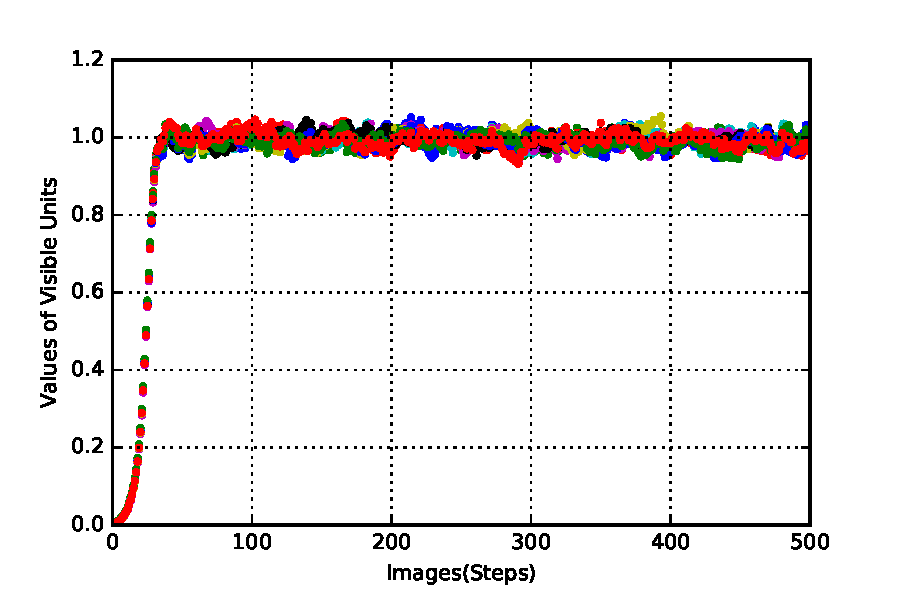
\includegraphics[width=\textwidth]{pics_sdlm/30_exp_RBM/exp1_recon_non.pdf}
		\caption{Reconstruction of visible units in Exp1}
	\end{subfigure}
	\begin{subfigure}[t]{0.48\textwidth}
		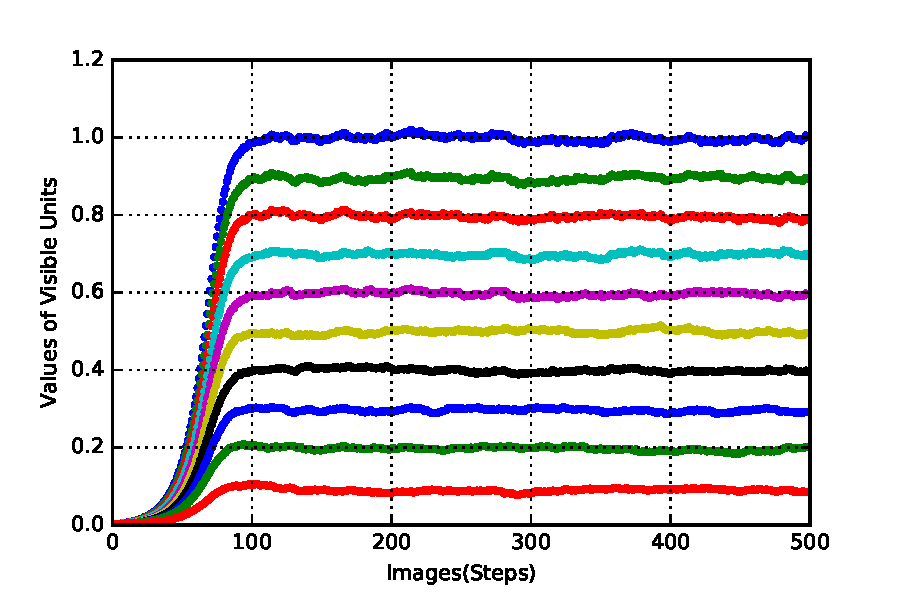
\includegraphics[width=\textwidth]{pics_sdlm/30_exp_RBM/exp2_recon_non.pdf}
		\caption{Reconstruction of visible units in Exp2}
	\end{subfigure}\\
	\begin{subfigure}[t]{0.48\textwidth}
		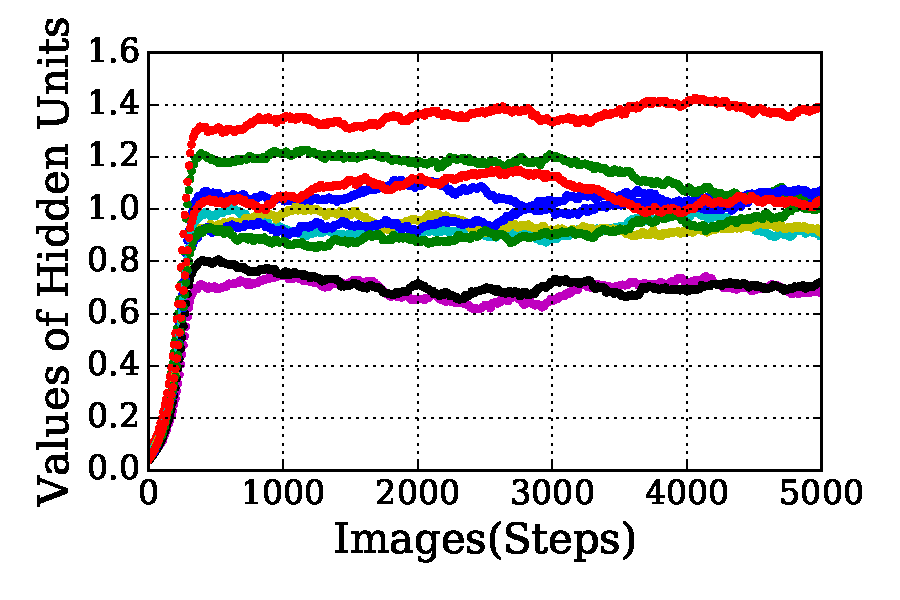
\includegraphics[width=\textwidth]{pics_sdlm/30_exp_RBM/exp1_hid_non.pdf}
		\caption{Output of hidden units in Exp1}
	\end{subfigure}
	\begin{subfigure}[t]{0.48\textwidth}
		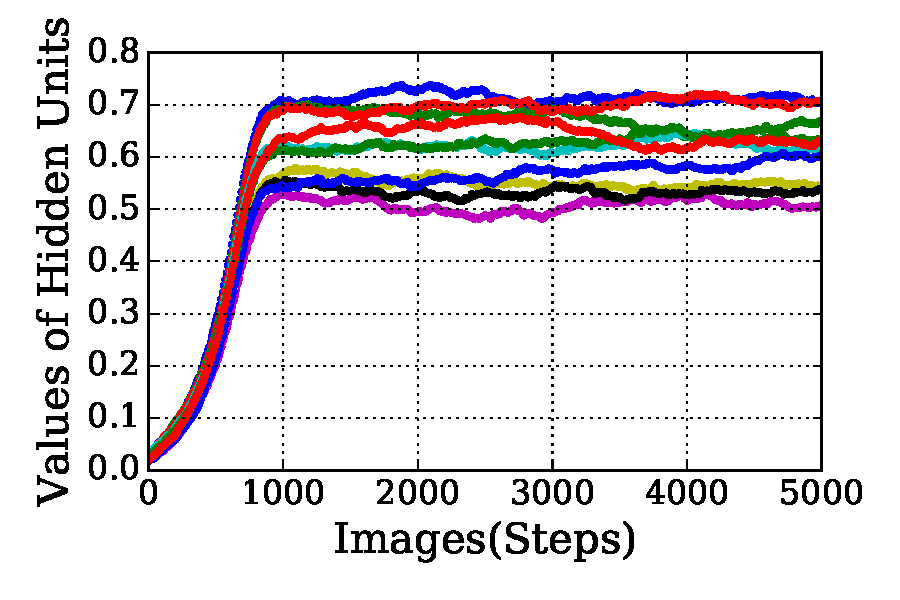
\includegraphics[width=\textwidth]{pics_sdlm/30_exp_RBM/exp2_hid_non.pdf}
		\caption{Output of hidden units in Exp2}
	\end{subfigure}\\
	\begin{subfigure}[t]{0.48\textwidth}
		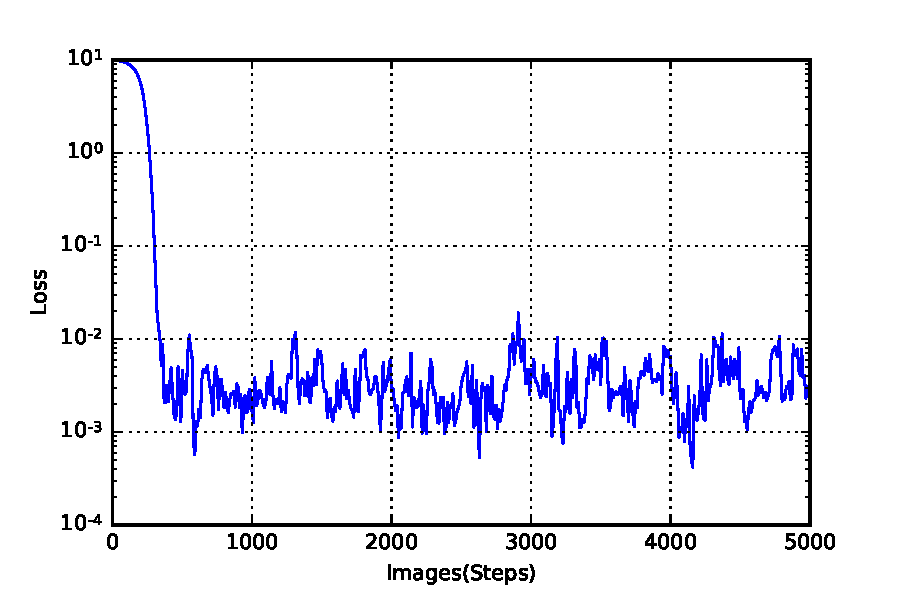
\includegraphics[width=\textwidth]{pics_sdlm/30_exp_RBM/exp1_loss.pdf}
		\caption{Output of hidden units in Exp1}
	\end{subfigure}
	\begin{subfigure}[t]{0.48\textwidth}
		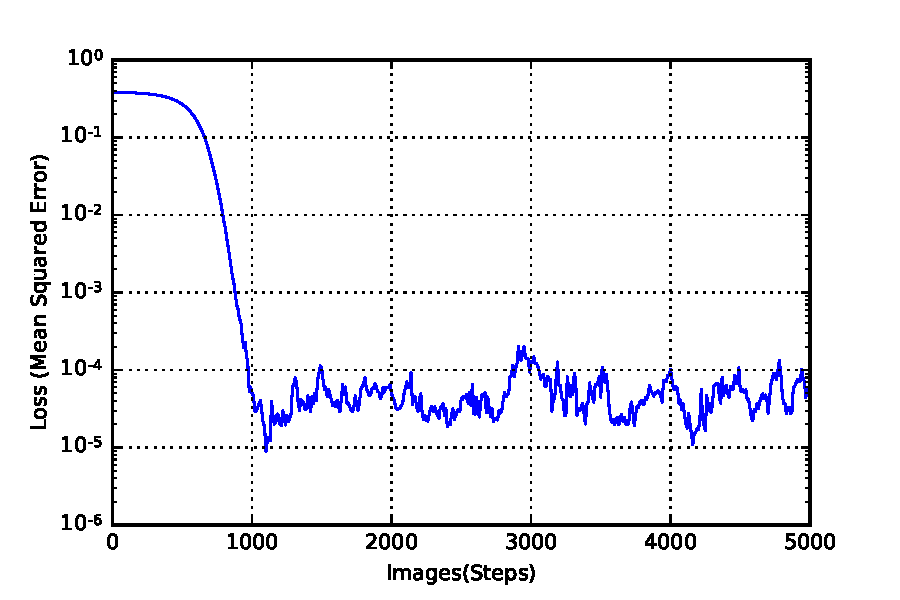
\includegraphics[width=\textwidth]{pics_sdlm/30_exp_RBM/exp2_loss.pdf}
		\caption{Output of hidden units in Exp2}
	\end{subfigure}
	\caption[nRBM training of the reconstruction tests.]{Changes of weights, output of visible and hidden units, and mean squared error (loss) during the nRBM training of the reconstruction tests. 
		Experiments 1) 10 visible units fully connected to 10 hidden units with input data of all 1s; 2) the same network fed with 10 values distributed linearly from 0.1 to 1.}
	\label{fig:rbm_orig}
\end{figure}

\begin{figure}
	\centering
	\begin{subfigure}[t]{0.48\textwidth}
		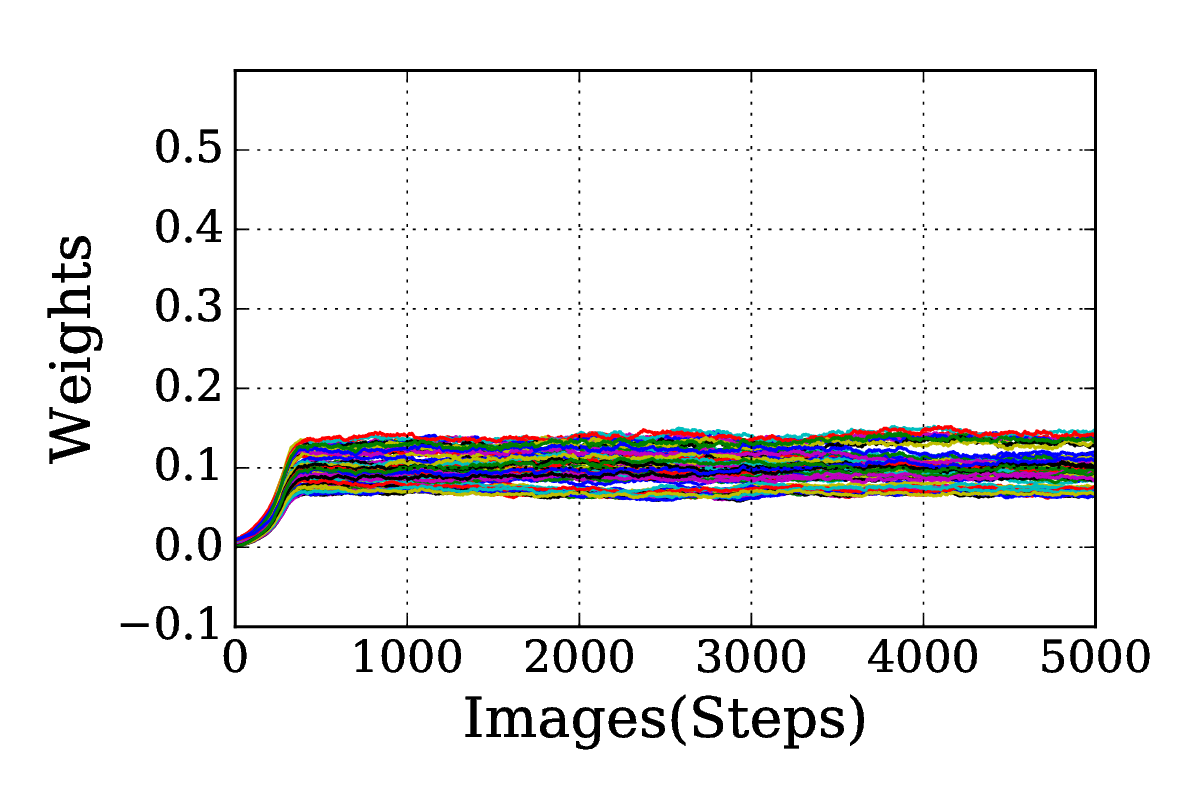
\includegraphics[width=\textwidth]{pics_sdlm/31_exp_RBM_noise/exp1_weights_s.png}
		\caption{Weights of Exp1}
	\end{subfigure}
	\begin{subfigure}[t]{0.48\textwidth}
		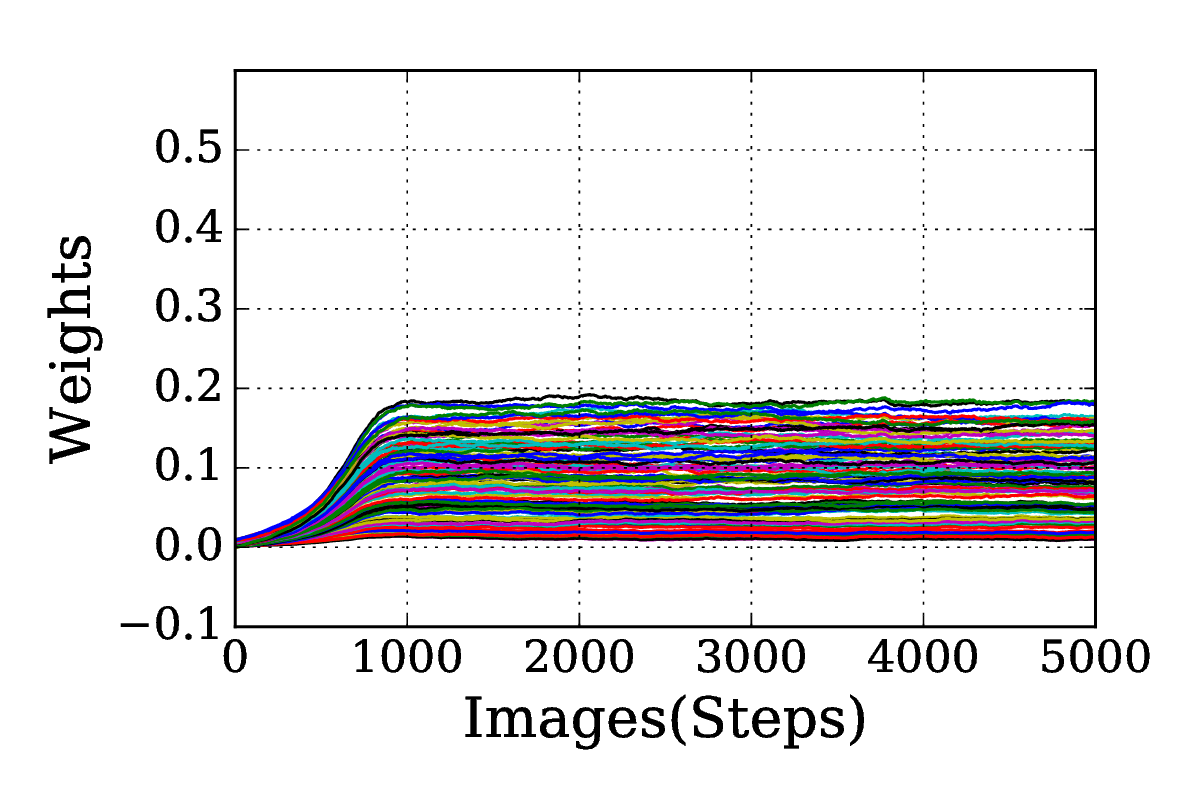
\includegraphics[width=\textwidth]{pics_sdlm/31_exp_RBM_noise/exp2_weights_s.png}
		\caption{Weights of Exp2}
	\end{subfigure}
	\begin{subfigure}[t]{0.48\textwidth}
		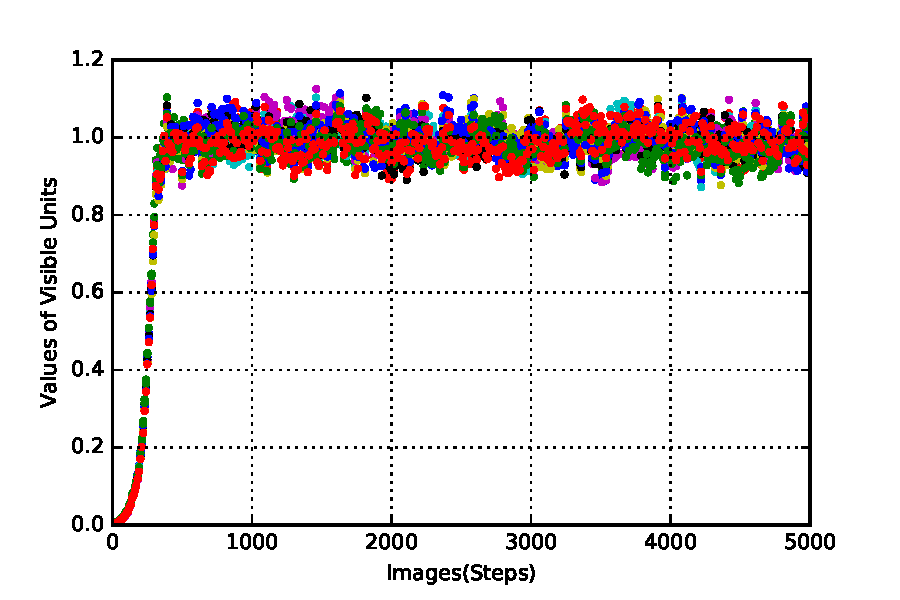
\includegraphics[width=\textwidth]{pics_sdlm/31_exp_RBM_noise/exp1_recon_s.pdf}
		\caption{Reconstruction of visible units in Exp1}
	\end{subfigure}
	\begin{subfigure}[t]{0.48\textwidth}
		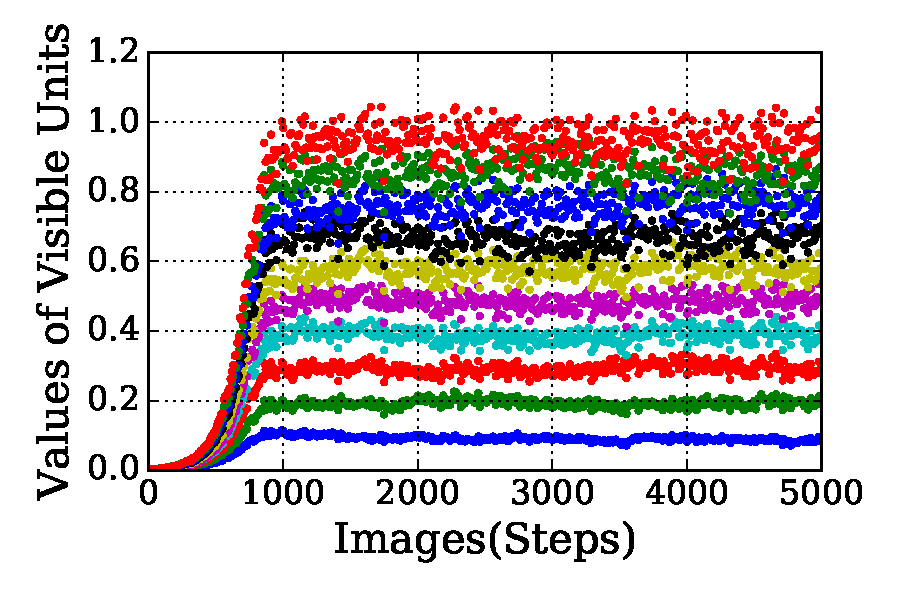
\includegraphics[width=\textwidth]{pics_sdlm/31_exp_RBM_noise/exp2_recon_s.pdf}
		\caption{Reconstruction of visible units in Exp2}
	\end{subfigure}\\
	\begin{subfigure}[t]{0.48\textwidth}
		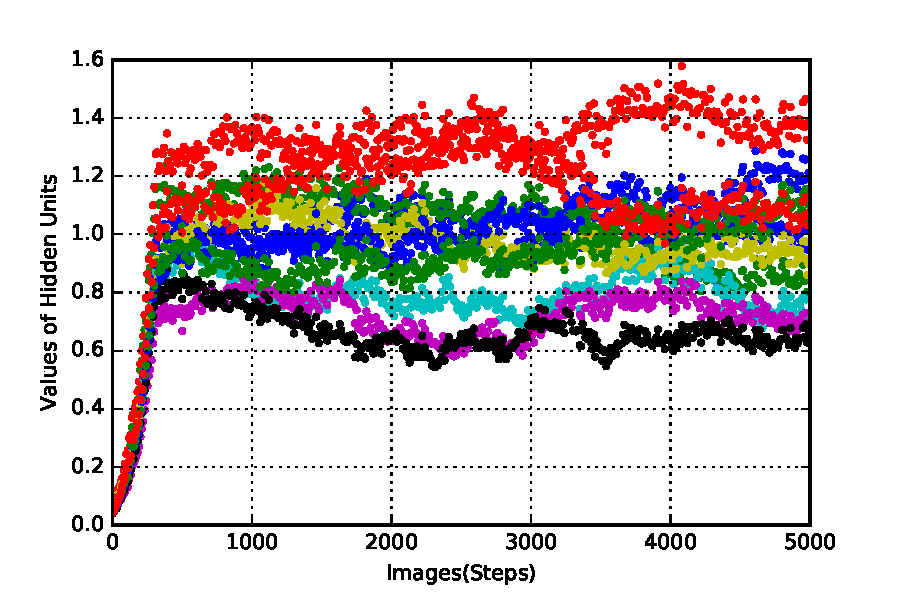
\includegraphics[width=\textwidth]{pics_sdlm/31_exp_RBM_noise/exp1_hid_s.pdf}
		\caption{Output of hidden units in Exp1}
	\end{subfigure}
	\begin{subfigure}[t]{0.48\textwidth}
		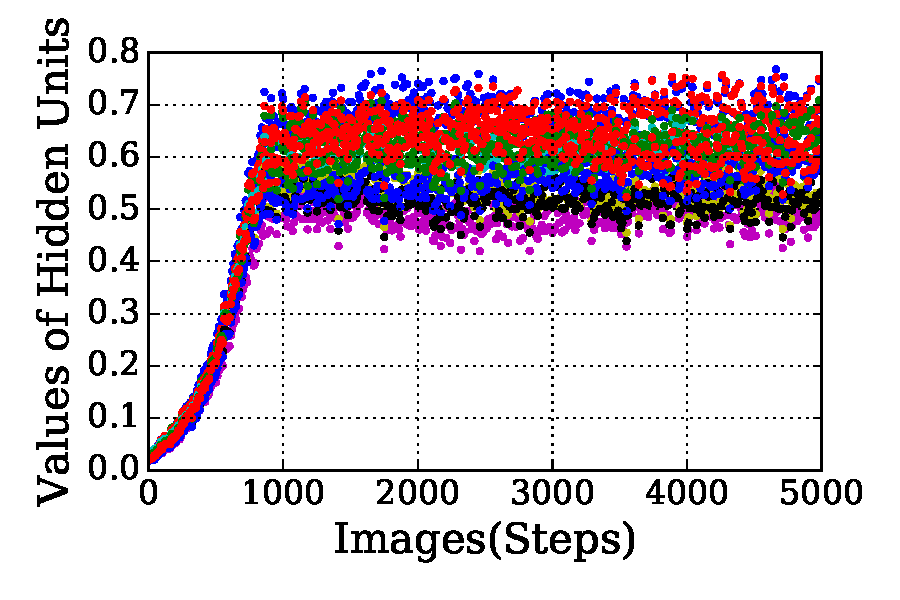
\includegraphics[width=\textwidth]{pics_sdlm/31_exp_RBM_noise/exp2_hid_s.pdf}
		\caption{Output of hidden units in Exp2}
	\end{subfigure}\\
	\begin{subfigure}[t]{0.48\textwidth}
		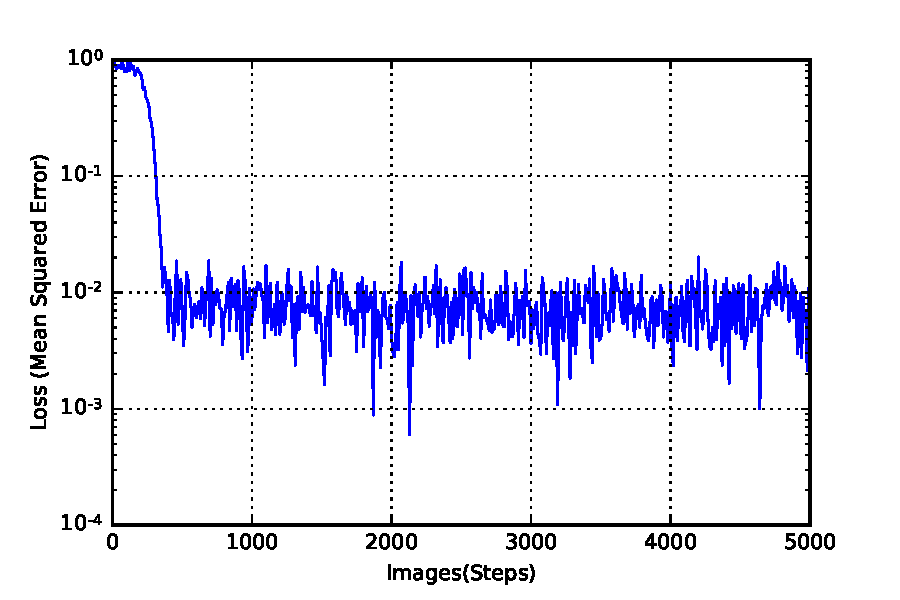
\includegraphics[width=\textwidth]{pics_sdlm/31_exp_RBM_noise/exp1_loss_s.pdf}
		\caption{Output of hidden units in Exp1}
	\end{subfigure}
	\begin{subfigure}[t]{0.48\textwidth}
		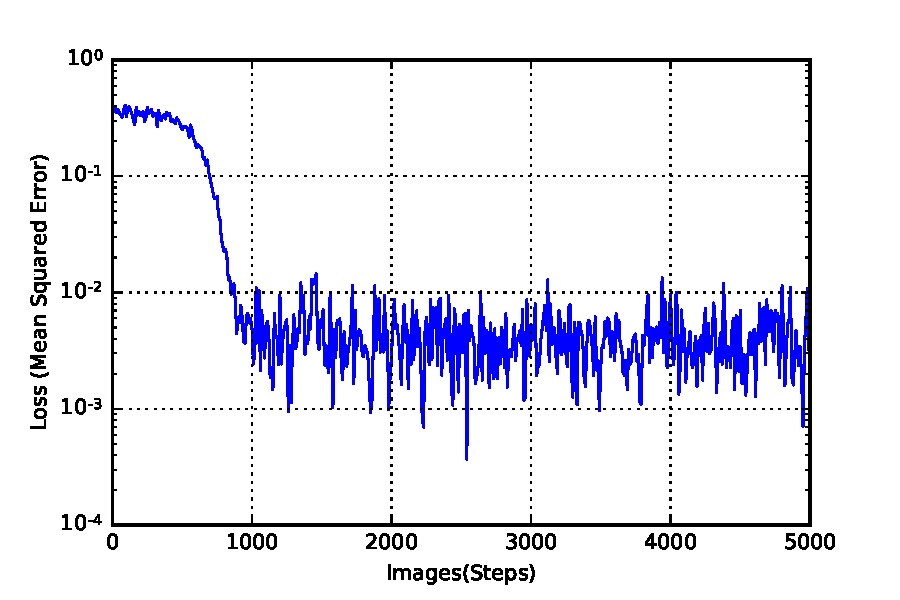
\includegraphics[width=\textwidth]{pics_sdlm/31_exp_RBM_noise/exp2_loss_s.pdf}
		\caption{Output of hidden units in Exp2}
	\end{subfigure}
	\DIFdelbeginFL %DIFDELCMD < \caption[nRBM training of the reconstruction tests given noisy data.]{%%%
\DIFdelendFL \DIFaddbeginFL \caption[nRBM-NI training of the reconstruction tests.]{\DIFaddendFL Changes of weights, output of visible and hidden units, and mean squared error (loss) during the nRBM training of the noisy reconstruction tests. 
		Experiments 1) 10 visible units fully connected to 10 hidden units with the count of Poisson spikes firing at 100~Hz which lasted 100~ms; 2) the same network fed with spike count of Poisson spikes at firing rate ranging from 10~Hz to 100~Hz.}
	\label{fig:rbm_noise}
\end{figure}

\DIFdelbegin %DIFDELCMD < \subsection{%%%
\DIFdelend \DIFaddbegin \subsection[Noisy RBMs]{\DIFadd{Training }\DIFaddend Noisy \DIFdelbegin \DIFdel{Restricted Boltzmann Machines (nRBMs)}\DIFdelend \DIFaddbegin \DIFadd{RBMs}\DIFaddend }
\label{subsec:exp_RBM}
Instead of using binary units and sigmoid activations for the RBM, we employed noisy ReLU (NReLU) units to construct an \DIFdelbegin \DIFdel{nRBM }\DIFdelend \DIFaddbegin \DIFadd{noisy Restricted Boltzmann Machine (nRBM) }\DIFaddend which was closer to biology and performed better in classification tasks~\citep{nair2010rectified}.
Leaving the learning algorithm unchanged, see Equation~\ref{equ:rbm_train} in Section~\ref{sec:rbm}\DIFaddbegin \DIFadd{, the weight update is as follows}\DIFaddend :
\begin{equation}
\Delta w_{ij} = \eta (h_iv_j - h'_iv'_j),
\label{equ:rbm}
\end{equation} 
where a Gibbs sample comprises a pare of $h'_i$ and $v'_j$, and the new sampling method NReLU is equivalent to generating multiple samples in the meantime and averaging them: $max(0, x+\mathcal{N}(0, \sigma(x))$.
The lower the variance of the normal distribution, the more samples are taken for averaging;
zero variance (equivalent to ReLU) is used when unlimited samples are generated, but at the same time the sampling itself loses the randomness.
In our experiments the variance of the normal distribution used in NReLU is 0.1 during training.
%While in testing, we used ReLU for the deterministic reconstructions. 
%To keep the similar network architecture and the learning rule with AEs, we used RBM with zero bias as well.
%Thus the weight updating rule in Equation~\ref{equ:rbm_train} can be described as:


Figure~\ref{fig:rbm_orig} demonstrates the training process and the test results of the nRBM; both experiments stabilises earlier than AE training: about 400 and $1,000$ steps respectively.
Due to the randomness of the sampling in the nRBM, there are noisy fluctuations in the weight change during training, the reconstructions and the output of hidden units in deterministic testing.
In addition, the loss stops declining at around $10^{-4}$ because of the same reason of randomness.

The same experiments were also carried out with the identical \DIFdelbegin \DIFdel{noisy input}\DIFdelend \DIFaddbegin \DIFadd{NI}\DIFaddend , see Figure~\ref{fig:rbm_noise}.
The weight change is slightly noisier than the experiments on clean data, but the noise is more obvious on the output of the visible reconstruction and the hidden units.
The same effect of the \DIFdelbegin \DIFdel{noisy input }\DIFdelend \DIFaddbegin \DIFadd{NI }\DIFaddend data can be found in Figure~\ref{fig:ae_noise} where the noise in the reconstruction is much reduced compared to the input data and the loss remains about $10^{-2}$ and $10^{-2.5}$ after the stabilisation, although it takes less time for the nRBM to converge than AE.


\DIFdelbegin %DIFDELCMD < \subsection{%%%
\DIFdelend \DIFaddbegin \subsection[Spiking AEs]{\DIFaddend Training Spiking \DIFdelbegin \DIFdel{Autoencoders (SAEs)}\DIFdelend \DIFaddbegin \DIFadd{AEs}\DIFaddend }
\label{subsec:exp_SAE}
Equation~\ref{equ:ae_widrow_hoff} states the learning rule for AEs, which can be approximated by adding a positive \DIFdelbegin \DIFdel{STDP }\DIFdelend and a negative STDP in SNN training:
\begin{equation}
\label{equ:sae}
\begin{aligned}
	\Delta w_{ij} &= \eta h_i v_j - \eta h_i v'_j \\
	&= \textit{\textrm{STDP}}(s_{h_i}, s_{v_j}) - \textit{\textrm{STDP}}(s_{h_i}, s_{v'_j})~ \\
	\textrm{where,~~} \eta_{s} &=  \frac{\eta 10^6}{K^2 \tau_{\textit{\textrm{dur}}} \tau_{\textit{\textrm{win}}}}~.
%	\textrm{~where}\\
%	&\left\{
%	\begin{aligned}
%	 \eta_{s+} &= \eta K^2 \tau_{\textit{\textrm{dur}}} \tau_{\textit{\textrm{win}}}10^{-6}~, ~\textrm{~when weights potentiate,~and}\\
%	 \eta_{s-} &= -\eta K^2 \tau_{\textit{\textrm{dur}}} \tau_{\textit{\textrm{win}}}10^{-6}~, ~\textrm{~when weights depress.}
%	 \end{aligned} 
%	 \right.
\end{aligned} 
\end{equation}
We use simple linear Integrate-and-Fire (IF) neurons to validate the training algorithm, whose membrane potential follows the dynamics:
\begin{equation}
V_i(t+1)=V_i(t) + \sum_j w_{ij} s_j(t)~,
\end{equation}
and an IF neuron fires when the membrane potential $V$ surpasses the membrane threshold $V_{thresh}$, and $V$ resets to $V_{rest}$ after firing or when it reduces below $V_{rest}$.
The parameters used are listed in Table~\ref{tbl:srm}.

\begin{table}[th]
	\centering
	\caption[Parameter setting of SRM.]{Parameter setting of SRM and IF neurons for training SAEs and SRBMs.}
	\bgroup
	\def\arraystretch{1.2}
	\begin{tabular}{c c l}
		%\hline
		Parameters & Values & Description \\
		\hline
		K & 100 & linear scaling factor\\
		%\hline
		$\tau_{\textit{\textrm{dur}}}$ & 100 ms &  length of training spike trains\\
		%\hline
		$\tau_{\textit{\textrm{win}}}$ & 10 ms & window length of STDP\\
		%\hline
		$\eta$ & $10^{-3}$ & learning rate of AEs and RBMs\\
		%\hline
		$\eta_{s+}$ & $10^{-4}$ & positive learning rate of SAEs and SRBMs\\
		$\eta_{s-}$ & $-10^{-4}$ & negative learning rate of SAEs and SRBMs\\
		%\hline
		$V_{rest}$ & 0~mV & resting membrane potential\\
		%\hline
		$V_{thresh}$ & 1~mV & membrane threshold  \\
	\end{tabular}
	\egroup
	\label{tbl:srm}
\end{table}

The weight increase takes place in the positive STDP learning between the neurons of the input ($\bf{v}$) and the hidden units ($\bf{h}$); 
the weight decrease is carried out in the negative STDP learning between the reconstruction ($\bf{v'}$) and the hidden neurons ($\bf{h}$).
Figure~\ref{fig:sym_conn} shows the network architecture of an SAE where the hidden units connect to the reconstruction neurons with the weight matrix $\bf{w}$ and the input neurons feedforward to the hidden layer with the transposed tied weights $\bf{w}^\textrm{T}$.
The shared weights, with the three individual populations of neurons, compose the training network of an SAE, see Figure~\ref{fig:rSTDP} (Left).

\begin{figure}[th]
	\centering
	\begin{subfigure}[t]{0.35\textwidth}
		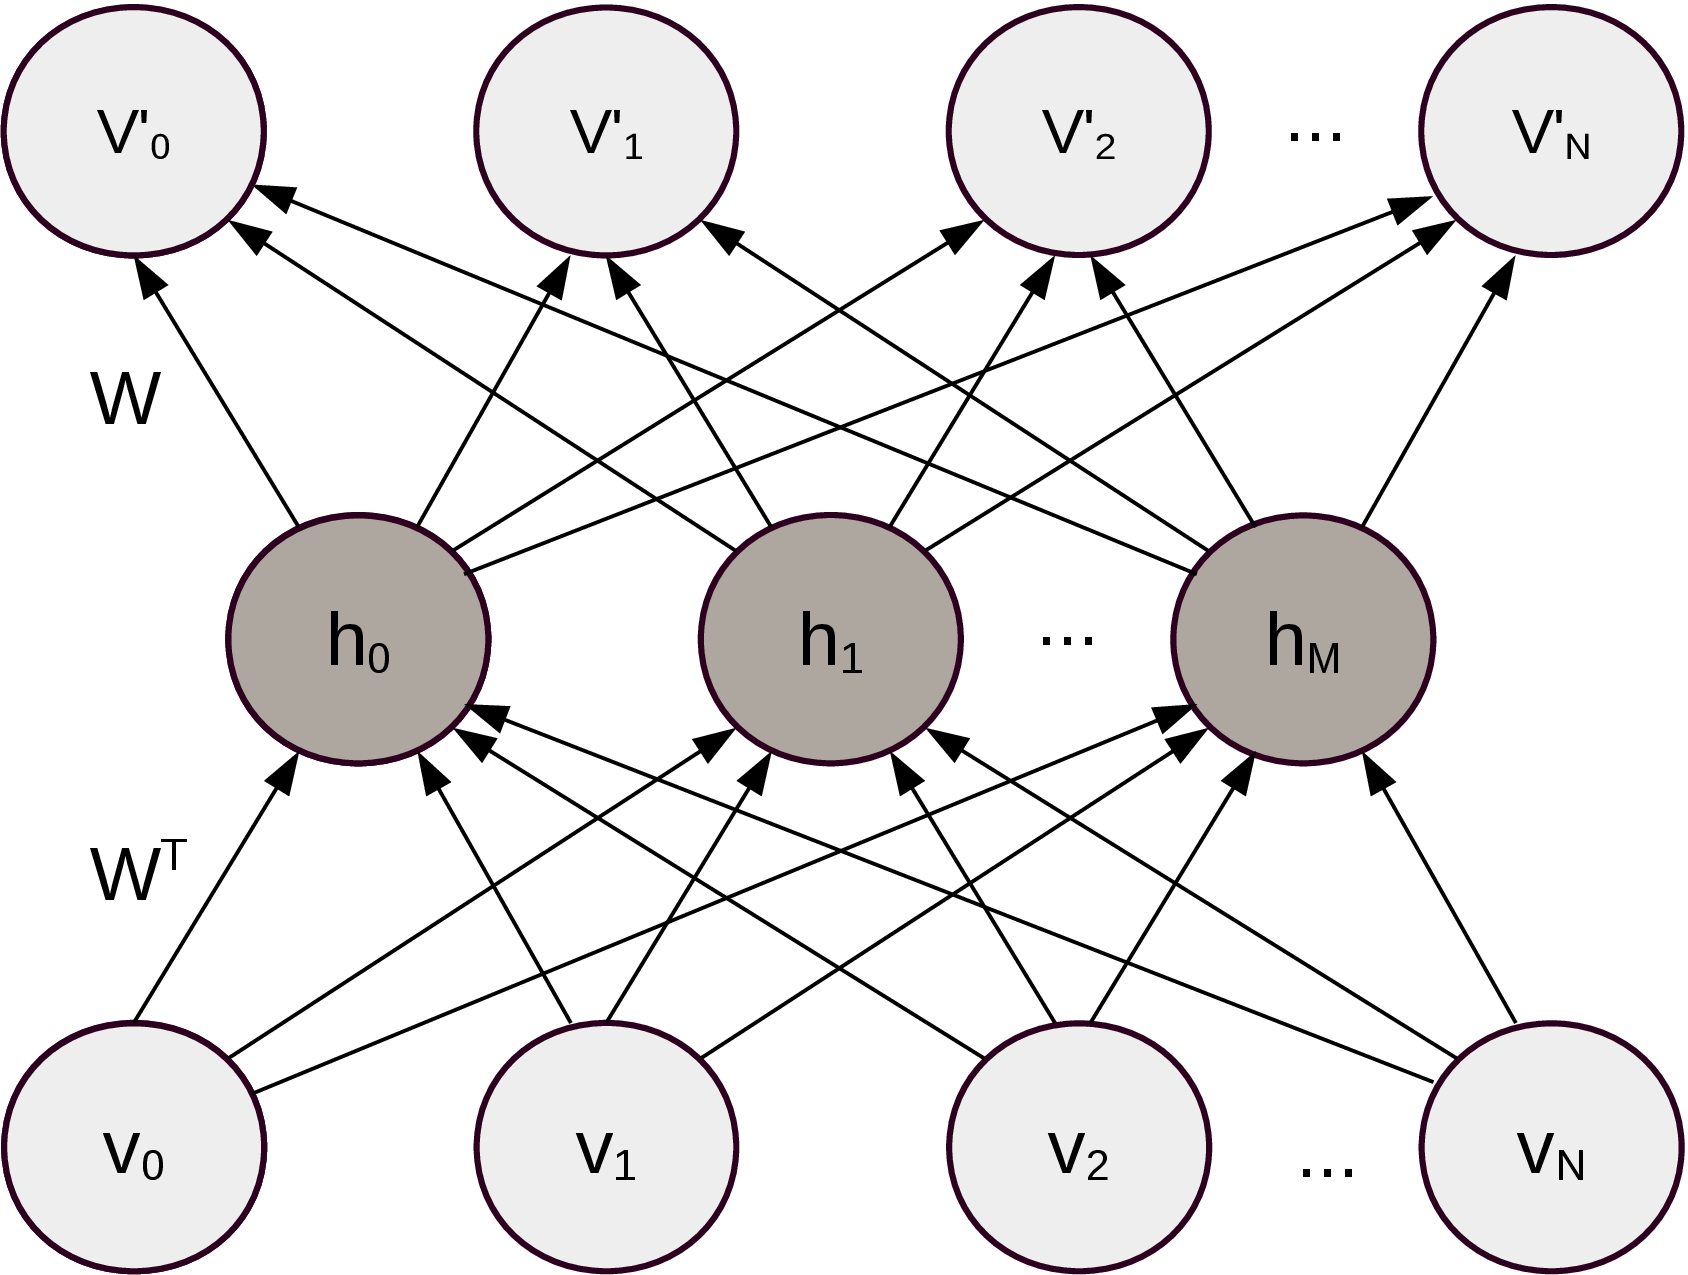
\includegraphics[width=\textwidth]{pics_sdlm/AE.png}
	\end{subfigure}
	\begin{subfigure}[t]{0.6\textwidth}
		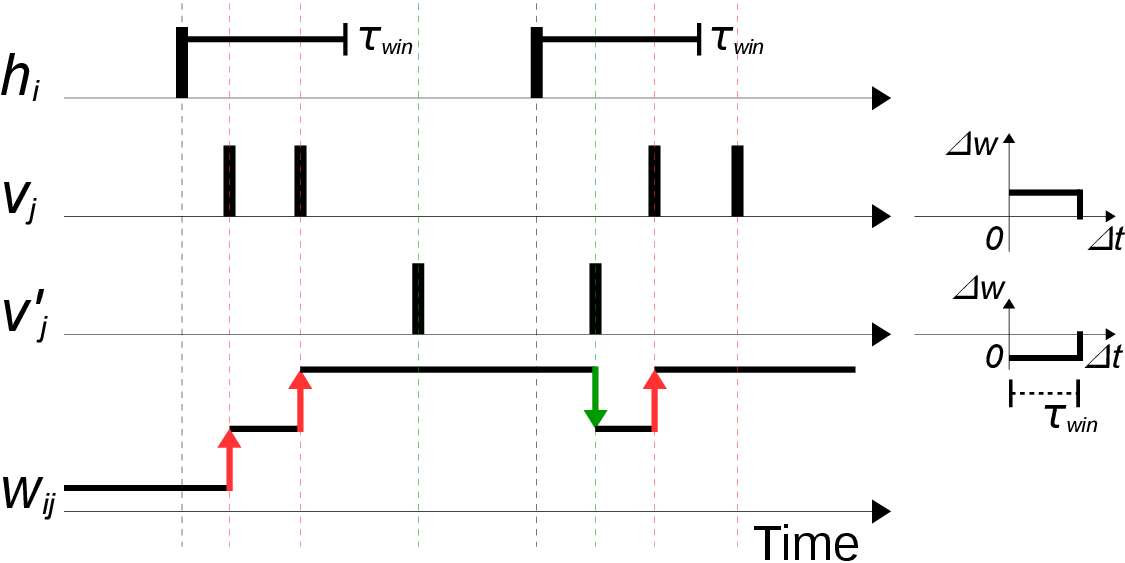
\includegraphics[width=\textwidth]{pics_sdlm/rSTDP.png}
	\end{subfigure}
	\caption{Network architecture and the learning algorithm of a spiking \DIFdelbeginFL \DIFdelFL{AEs}\DIFdelendFL \DIFaddbeginFL \DIFaddFL{AE}\DIFaddendFL .}
	\label{fig:rSTDP}
\end{figure}

\begin{figure}
	\centering
	\begin{subfigure}[t]{0.48\textwidth}
		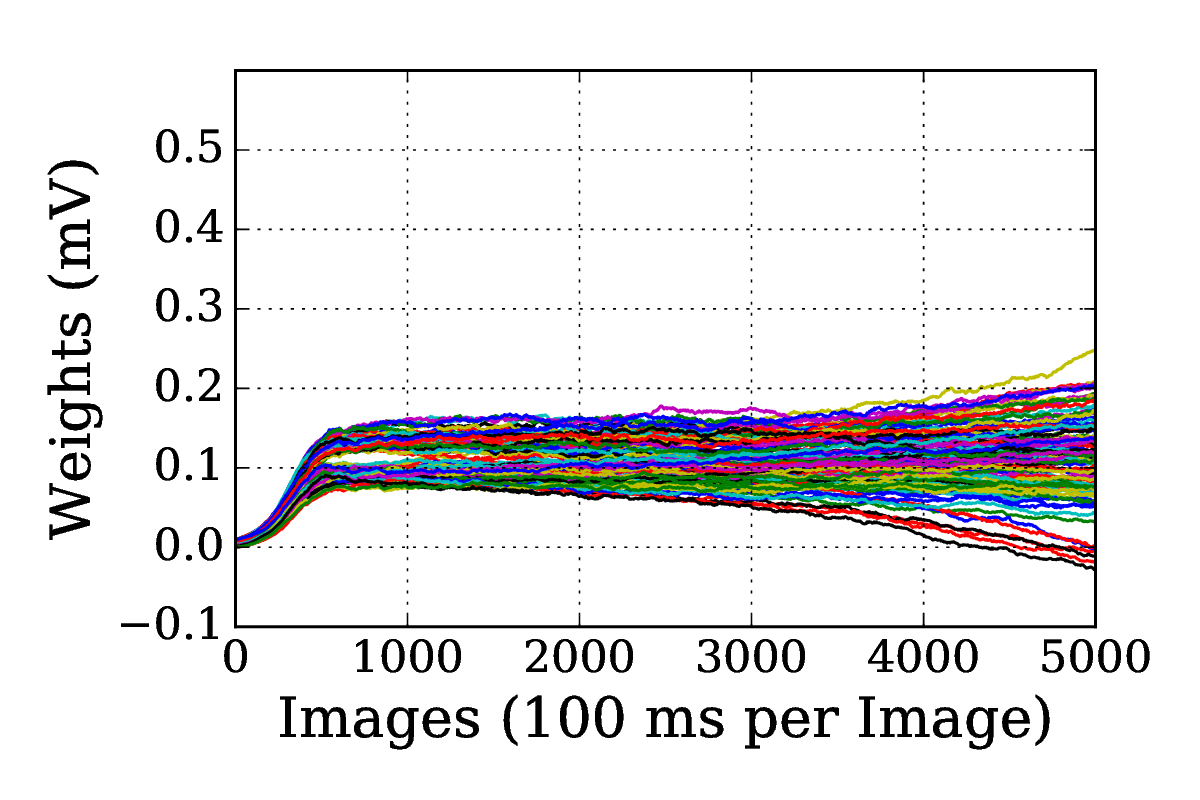
\includegraphics[width=\textwidth]{pics_sdlm/00_exp_SAE_Orig/exp1_weights_s.png}
		\caption{Weights of Exp1}
	\end{subfigure}
	\begin{subfigure}[t]{0.48\textwidth}
		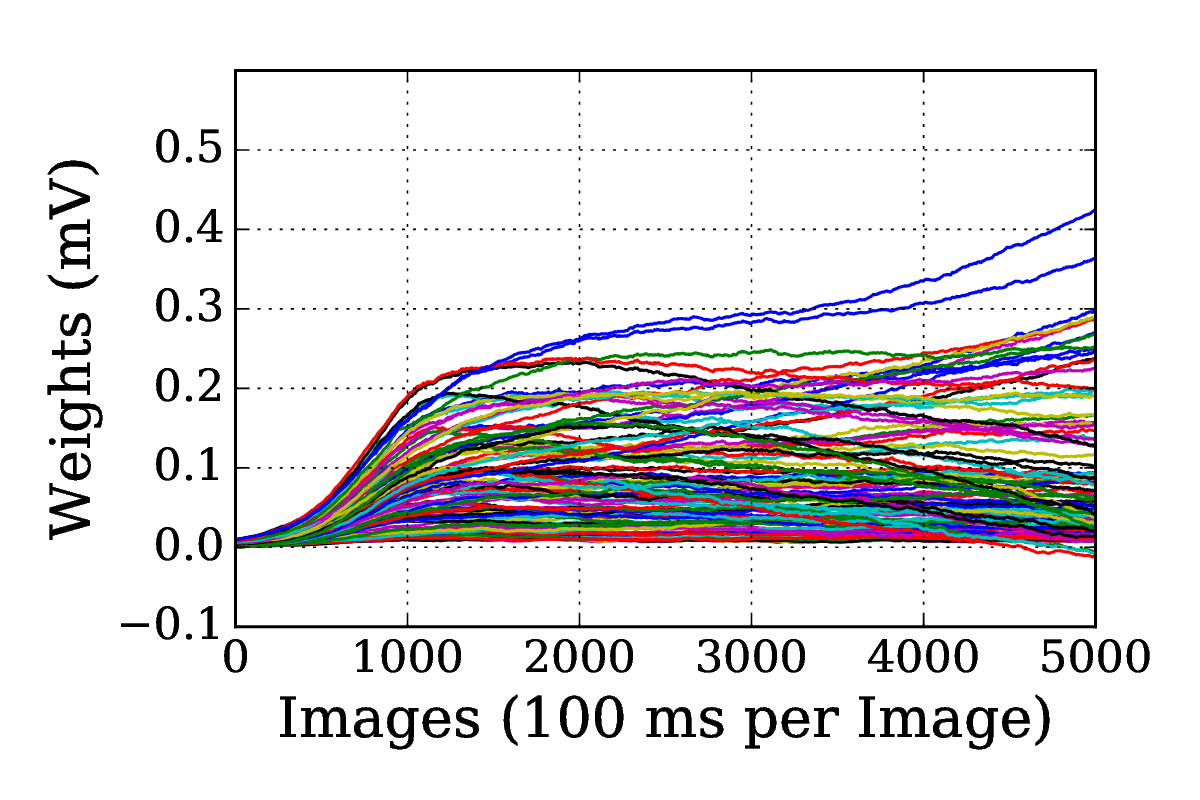
\includegraphics[width=\textwidth]{pics_sdlm/00_exp_SAE_Orig/exp2_weights_s.png}
		\caption{Weights of Exp2}
	\end{subfigure}
	\begin{subfigure}[t]{0.48\textwidth}
		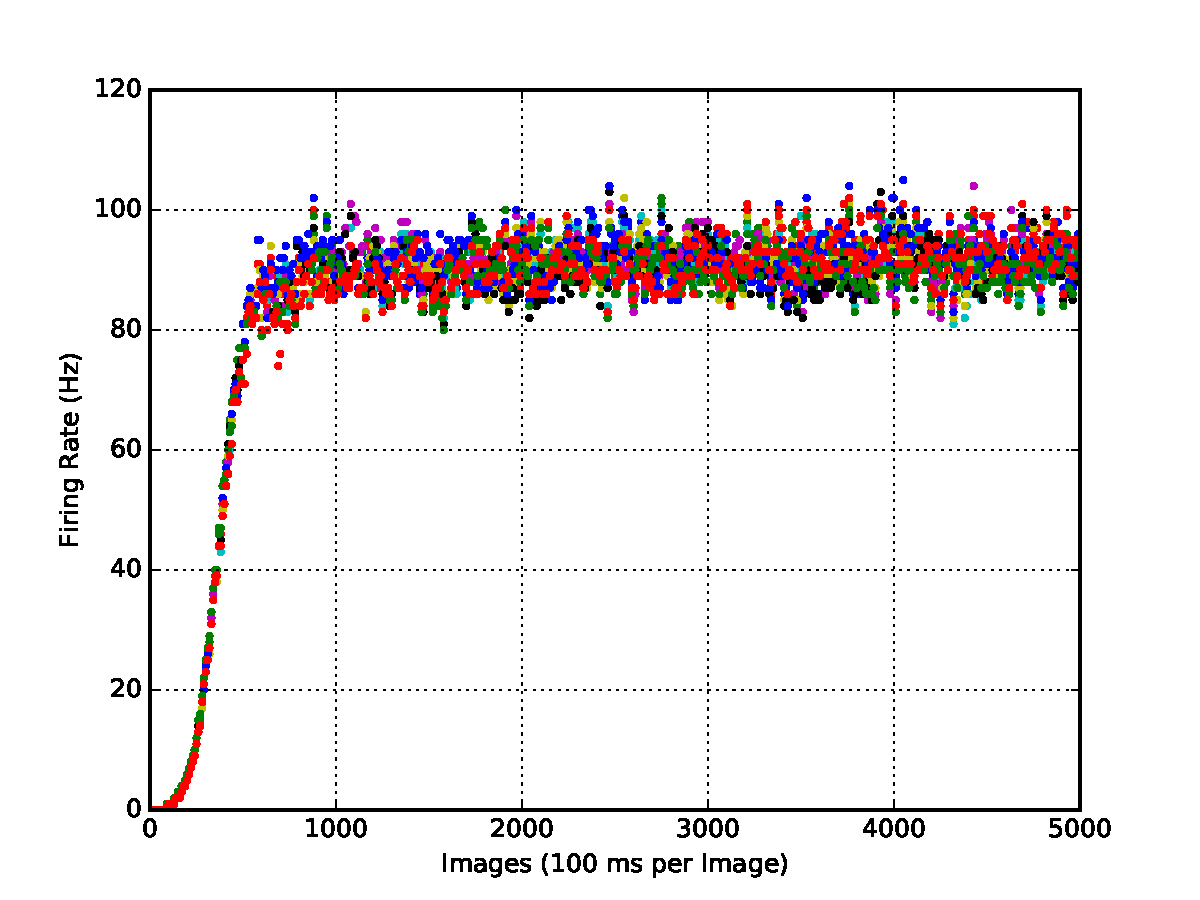
\includegraphics[width=\textwidth]{pics_sdlm/00_exp_SAE_Orig/exp1_recon_s.pdf}
		\caption{Reconstruction of visible units in Exp1}
	\end{subfigure}
	\begin{subfigure}[t]{0.48\textwidth}
		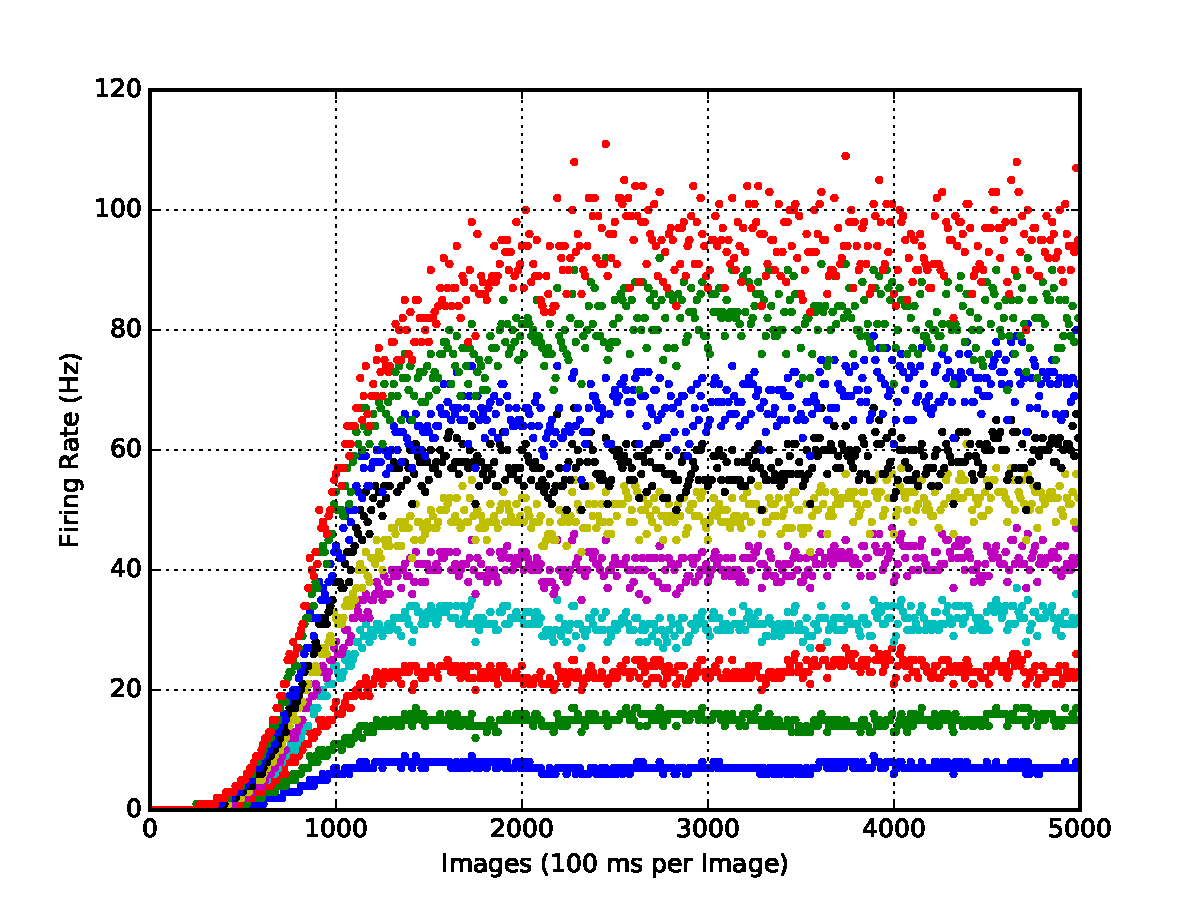
\includegraphics[width=\textwidth]{pics_sdlm/00_exp_SAE_Orig/exp2_recon_s.pdf}
		\caption{Reconstruction of visible units in Exp2}
	\end{subfigure}\\
	\begin{subfigure}[t]{0.48\textwidth}
		\includegraphics[width=\textwidth]{pics_sdlm/00_exp_SAE_Orig/exp1_hid_s.pdf}
		\caption{Output of hidden units in Exp1}
	\end{subfigure}
	\begin{subfigure}[t]{0.48\textwidth}
		\includegraphics[width=\textwidth]{pics_sdlm/00_exp_SAE_Orig/exp2_hid_s.pdf}
		\caption{Output of hidden units in Exp2}
	\end{subfigure}\\
	\begin{subfigure}[t]{0.48\textwidth}
		\includegraphics[width=\textwidth]{pics_sdlm/00_exp_SAE_Orig/exp1_mse_nons.pdf}
		\caption{Loss of Exp1}
	\end{subfigure}
	\begin{subfigure}[t]{0.48\textwidth}
		\includegraphics[width=\textwidth]{pics_sdlm/00_exp_SAE_Orig/exp2_mse_nons.pdf}
		\caption{Loss of Exp2}
	\end{subfigure}
	\caption[SAE training of the reconstruction tests.]{Weights and firing rates of visible and hidden units change during training of the reconstruction tests of the spiking AE. 
		Experiments 1) 10 visible units fully connected to 10 hidden units with Poisson spike trains of 100~Hz which lasted 100~ms; 2) the same network fed with 10 Poisson spike trains of firing rate ranging from 10~Hz to 100~Hz.}
	\label{fig:SAE_orig}
\end{figure}

Figure~\ref{fig:rSTDP} (Right) illustrates the learning mechanism of the SAE architecture by giving an example of one hidden neuron $h_i$ connected to an input neuron $v_j$ and connecting to a reconstruction neuron $v'_j$ with the same strength $w_{ij}$.
The weight $w_{ij}$ rises by $\eta_{s+}$ (marked with an up-arrow) when a spike comes within the period of $\tau_{\textit{\textrm{win}}}$ after the hidden neuron fires;
and it decreases by $\eta_{s-}$ (marked with a down-arrow) if the reconstruction neuron generates a spike in the same time window.
If either $v_j$ or $v'_j$ spikes outside the effective STDP window, the weight will remain unchanged.
The learning continues as long as the neurons are active, however the weights may stay relatively stable when the input firing rate is the same as the reconstruction's.

To reproduce the experiments of the AEs, we selected the parameters (see Table~\ref{tbl:srm}) for training SAEs and also apply the same parameters for SRBM experiments.
Each input vector (image) was presented as spiking trains with the length of 100~ms, and the STDP window was set to 10~ms.
The input values scaled up by $K=100$~Hz were used as firing rates of the spike trains.
Therefore, according to Equation~\ref{equ:srm}, the learning rate of SAEs and SRBMs was $\pm 10^{-4}$.

To compare with the AE experiments on \DIFdelbegin \DIFdel{noisy input }\DIFdelend \DIFaddbegin \DIFadd{NI }\DIFaddend data, Figure~\ref{fig:SAE_orig} records the weight change during training and the results generated by the testing on each image presented for 1~s.
The most important and obvious difference is the weight change where the weights do not stabilise but their values diverge during training.
%The output firing rate of the hidden units tends to converge as training procedes on.
The reason for the phenomena will be discussed in Section~\ref{sec:problem}.
The training is slower than the AE experiments and the loss takes longer to decrease to the same level.
This is mainly caused by the low firing rate of both input and hidden units at the beginning of the training.
Thus, few, even no, spikes triggered STDP.
With the simple input of Exp1, the training performance reaches the same level of 0.01 loss compared to the noisy AE test;
however, the SAE does not reconstruct the various input values of Exp2 as accurately as does the AE, since the parameters $\tau_{\textit{\textrm{win}}}$ and $\tau_{\textit{\textrm{dur}}}$ are relatively short.
We will present more results conducted with various parameter settings in Section~\ref{sec:problem}.

\DIFdelbegin %DIFDELCMD < \subsection{%%%
\DIFdelend \DIFaddbegin \subsection[Spiking RBMs]{\DIFaddend Training Spiking \DIFdelbegin \DIFdel{RBM}\DIFdelend \DIFaddbegin \DIFadd{RBMs}\DIFaddend }
\label{subsec:exp_SRBM}
\begin{figure}[h]
	\centering
		\begin{subfigure}[c]{0.33\textwidth}
			\includegraphics[width=\textwidth]{pics_sdlm/rbm.png}
		\end{subfigure}
		\begin{subfigure}[c]{0.66\textwidth}
			\includegraphics[width=\textwidth]{pics_sdlm/rSTDP_rbm.png}
		\end{subfigure}
	\caption{Network architecture and the learning algorithm of a spiking RBM.}
	\label{fig:sRBM}
\end{figure}

As illustrated in Equation~\ref{equ:rbm}, the positive weight change is generated from the multiplication of the visible and hidden units where the weight depression comes from the product of the Gibbs sampled hidden and reconstruction values.
Figure~\ref{fig:sRBM} shows the architecture of an SRBM which consists of four layers of neurons: input $\bf{v}$, hidden layer $\bf{h}$, Gibbs visible (or reconstruction) $\bf{v'}$ and Gibss hidden $\bf{h'}$ neurons, and the shared weights $\bf{W}$.

\begin{figure}
	\centering
	\begin{subfigure}[t]{0.48\textwidth}
		\includegraphics[width=\textwidth]{pics_sdlm/10_exp_SRBM_Orig/exp1_weights_s.png}
		\caption{Weights of Exp1}
	\end{subfigure}
	\begin{subfigure}[t]{0.48\textwidth}
		\includegraphics[width=\textwidth]{pics_sdlm/10_exp_SRBM_Orig/exp2_weights_s.png}
		\caption{Weights of Exp2}
	\end{subfigure}
	\begin{subfigure}[t]{0.48\textwidth}
		\includegraphics[width=\textwidth]{pics_sdlm/10_exp_SRBM_Orig/exp1_recon_s.pdf}
		\caption{Reconstruction of visible units in Exp1}
	\end{subfigure}
	\begin{subfigure}[t]{0.48\textwidth}
		\includegraphics[width=\textwidth]{pics_sdlm/10_exp_SRBM_Orig/exp2_recon_s.pdf}
		\caption{Reconstruction of visible units in Exp2}
	\end{subfigure}\\
	\begin{subfigure}[t]{0.48\textwidth}
		\includegraphics[width=\textwidth]{pics_sdlm/10_exp_SRBM_Orig/exp1_hid_s.pdf}
		\caption{Output of hidden units in Exp1}
	\end{subfigure}
	\begin{subfigure}[t]{0.48\textwidth}
		\includegraphics[width=\textwidth]{pics_sdlm/10_exp_SRBM_Orig/exp2_hid_s.pdf}
		\caption{Output of hidden units in Exp2}
	\end{subfigure}\\
	\begin{subfigure}[t]{0.48\textwidth}
		\includegraphics[width=\textwidth]{pics_sdlm/10_exp_SRBM_Orig/exp1_mse_nons.pdf}
		\caption{Loss of Exp1}
	\end{subfigure}
	\begin{subfigure}[t]{0.48\textwidth}
		\includegraphics[width=\textwidth]{pics_sdlm/10_exp_SRBM_Orig/exp2_mse_nons.pdf}
		\caption{Loss of Exp2}
	\end{subfigure}
	\caption[SRBM training of the reconstruction tests.]{Weights and firing rates of visible and hidden units change during training of the reconstruction tests of the spiking RBM. 
		Experiments 1) 10 visible units fully connected to 10 hidden units with Poisson spike trains of 100~Hz which lasted 100~ms; 2) the same network fed with 10 Poisson spike trains of firing rate ranging from 10~Hz to 100~Hz.}
	\label{fig:srbm_orig}
\end{figure}

Figure~\ref{fig:sRBM} demonstrates the training of an SRBM with a pair of spiking neurons $v_j$ and $h_i$, the corresponding \DIFdelbegin \DIFdel{to }\DIFdelend the Gibbs sampling pair $v'_j$ and $h'_i$, and the shared weight $w_{ij}$.
Up-arrows mark the increase of the weight when $v_j$ fires during the time window after the spikes of $h_i$;
meanwhile, down-arrows highlight	 the weight depression when $v'_j$ generates a spike no later than $\tau_{\textit{\textrm{win}}}$ after $h'_i$ fires.
%The amplitudes of the weight change, $\eta_{s+}$ and $\eta_{s-}$, were set the same as in Table~\ref{tbl:srm}.


%\begin{figure}
%	\centering
%	\includegraphics[width=0.7\textwidth]{pics_sdlm/rSTDP_rbm.pdf}
%	\caption{How SRM works in training spiking RBMs.}
%	\label{fig:rSTDP_rbm}
%\end{figure}





Weight divergence is a more severe problem in the SRBM, see Figure~\ref{fig:srbm_orig}.
Especially for Exp1, only one hidden neuron is active on the later half of the training, thus making the firing rate of the reconstruction jump between two states.
Because of the high firing rate of the pre-synaptic neuron, a slight weight increase may generate quite a few spikes for the post-synaptic neuron.
Therefore, more balanced activity among hidden neurons can perform better in terms of reconstruction accuracy.
%The same as SAE experiments, the slower training and worse loss also appear in the experiments.

\section{Problem of Spike Correlations	}
\label{sec:problem}
From the experiments above, the problem of the non-convergence of weight searching appears in training of SAEs and SRBMs using SRM.
Instead of stabilising at a (local) minimum of the parameter space, the values of the weights continue to grow or to decay, in fact to diverge, even after the loss locks to a certain level.
The diverging weights not only make the loss increase, for example as shown in Figure~\ref{fig:srbm_orig}(g), but also lead the weights too far from the expected effective range of the conventional AE or RBM training.

The diverging weight values are caused by correlations between spike trains.
Note that the rate multiplication of two spike trains (stated in Equation~\ref{equ:mul}) works under the condition of the independence of the spike trains.
However, the spike trains generated by a layer of neurons are strongly correlated to the spikes which the lower layer feeds them; and also influence the spike firing of the upper layer.
Therefore, any pair of spike trains $\bf{v}$ and $\bf{h}$, and $\bf{h}$ and $\bf{v'}$ in training SAEs are correlated, so are the spikes of $\bf{h'}$ and $\bf{v'}$ of SRBMs.


Taking SAE training for example, the strength of some synapses continuously increases because they have a relatively strong weight to trigger hidden units to fire, but the hidden units taking their transposed weights have a weaker impact on the firing of the reconstruction neuron.
Thus the correlation between $v_j$ and $h_i$ is stronger than between $v'_j$ and $h_i$, making the positive weight update more frequently than it drops.
On the contrary, the decreasing weights appear in the opposite situation when $h_i$ correlates stronger with $v'_j$ than $v_j$.
Regarding the SRBM, the training is even more effected by the correlations where the values of the weights diverge faster.

 
This section proposes four solutions to reduce the correlation between spike trains, thereby approximating AE and RBM training with equivalent spike-based on-line learning of SAEs and SRBMs.
%training spiking Deep Learning models approximately to the process of their conventional training methods.
%The aim is to modulate the weight updates close to AE and RBM training under the premise of keeping a similar level of loss.
To highlight the performance of the solutions, we apply these methods to the same experiments above, and the default parameters are the same as in Table~\ref{tbl:srm}.
\begin{figure}
	\centering
	\begin{subfigure}[c]{0.48\textwidth}\raggedleft
		\myrowlabel{Orignal SAE}
		\raisebox{-.5\height}{\includegraphics[width=.9\textwidth]
			{pics_sdlm/00_exp_SAE_Orig/exp2_weights_s.png}}\\
		\myrowlabel{S1}
		\raisebox{-.5\height}{\includegraphics[width=.9\textwidth]
			{pics_sdlm/01_exp_SAE_Orig_long/exp2_weights_s.png}}\\
		\myrowlabel{S2}
		\raisebox{-.5\height}{\includegraphics[width=.9\textwidth]
			{pics_sdlm/03_exp_SAE_noise_long/exp2_weights_s.png}}
		\myrowlabel{S3}
		\raisebox{-.5\height}{\includegraphics[width=.9\textwidth]
			{pics_sdlm/05_exp_SAE_teach_long/exp2_weights_s.png}}\\
		\myrowlabel{S4}
		\raisebox{-.5\height}{\includegraphics[width=.9\textwidth]
			{pics_sdlm/07_exp_SAE_all_long/exp2_weights_s.png}}
		\caption{Exp2 Weights}
	\end{subfigure}%
	\hspace{1em}
	\begin{subfigure}[c]{0.48\textwidth}\raggedleft
		\raisebox{-.5\height}{\includegraphics[width=.9\textwidth]
			{pics_sdlm/00_exp_SAE_Orig/exp2_mse_nons.pdf}}\\
		\raisebox{-.5\height}{\includegraphics[width=.9\textwidth]
			{pics_sdlm/01_exp_SAE_Orig_long/exp2_mse_nons.pdf}}\\
		\raisebox{-.5\height}{\includegraphics[width=.9\textwidth]
			{pics_sdlm/03_exp_SAE_noise_long/exp2_mse_nons.pdf}}
		\raisebox{-.5\height}{\includegraphics[width=.9\textwidth]
			{pics_sdlm/05_exp_SAE_teach_long/exp2_mse_nons.pdf}}\\
		\raisebox{-.5\height}{\includegraphics[width=.9\textwidth]
			{pics_sdlm/07_exp_SAE_all_long/exp2_mse_nons.pdf}}
		\caption{Exp2 Loss}
	\end{subfigure}%
	\caption[Comparisons of solutions in training SAE.]{Comparisons of weights and loss of solutions for training SAE on Exp2: [S1] longer STDP window, [S2] noisy threshold, [S3] teaching signal, and [S4] combined solutions. 10 visible units fully connects to 10 hidden units with Poisson spike trains of firing rate ranging from 10~Hz to 100~Hz.}
	\label{fig:sols_ae}
\end{figure}

\begin{figure}
	\centering
	\begin{subfigure}[c]{0.48\textwidth}\raggedleft
		\myrowlabel{Orignal SRBM}
		\raisebox{-.5\height}{\includegraphics[width=.9\textwidth]
			{pics_sdlm/10_exp_SRBM_Orig/exp2_weights_s.png}}\\
		\myrowlabel{S1}
		\raisebox{-.5\height}{\includegraphics[width=.9\textwidth]
			{pics_sdlm/11_exp_SRBM_Orig_long/exp2_weights_s.png}}\\
		\myrowlabel{S2}
		\raisebox{-.5\height}{\includegraphics[width=.9\textwidth]
			{pics_sdlm/13_exp_SRBM_noise_long/exp2_weights_s.png}}
		\myrowlabel{S3}
		\raisebox{-.5\height}{\includegraphics[width=.9\textwidth]
				{pics_sdlm/15_exp_SRBM_teach_long/exp2_weights_s.png}}\\
		\myrowlabel{S4}
		\raisebox{-.5\height}{\includegraphics[width=.9\textwidth]
			{pics_sdlm/17_exp_SRBM_all_long/exp2_weights_s.png}}
		\caption{Exp2 Weights}
	\end{subfigure}%
	\hspace{1em}
	\begin{subfigure}[c]{0.48\textwidth}\raggedleft
		\raisebox{-.5\height}{\includegraphics[width=.9\textwidth]
			{pics_sdlm/10_exp_SRBM_Orig/exp2_mse_nons.pdf}}\\
		\raisebox{-.5\height}{\includegraphics[width=.9\textwidth]
			{pics_sdlm/11_exp_SRBM_Orig_long/exp2_mse_nons.pdf}}\\
		\raisebox{-.5\height}{\includegraphics[width=.9\textwidth]
			{pics_sdlm/13_exp_SRBM_noise_long/exp2_mse_nons.pdf}}
		\raisebox{-.5\height}{\includegraphics[width=.9\textwidth]
			{pics_sdlm/15_exp_SRBM_teach_long/exp2_mse_nons.pdf}}\\
		\raisebox{-.5\height}{\includegraphics[width=.9\textwidth]
			{pics_sdlm/17_exp_SRBM_all_long/exp2_mse_nons.pdf}}
		\caption{Exp2 Loss}
	\end{subfigure}%
	\caption[Comparisons of solutions in training SRBM.]{Comparisons of weights and loss of solutions for training SRBM on Exp2: [S1] longer STDP window, [S2] noisy threshold, [S3] teaching signal, and [S4] combined solutions. 10 visible units fully connects to 10 hidden units with Poisson spike trains of firing rate ranging from 10~Hz to 100~Hz.}
	\label{fig:sols_rbm}
\end{figure}

\subsection{Solution~1~(S1): Longer STDP Window}
A stronger weight between a pair of pre- and post-synaptic neurons results in a higher probability for the pre-synaptic neuron to trigger a post-synaptic spike in a shorter period; 
%v and h can be reversed in experiments! maybe show some result.
a weaker connection strength usually takes longer to activate a spike.
Thus SRM using a short $\tau_{\textit{\textrm{win}}}$ produces a lower rate multiplication than the numerical product, especially for the weak weights.
Therefore, we use a longer square STDP window to accumulate more evidence to improve the accuracy of SRM, thus to make SRM more independent of the correlations between spike trains.
Of course, an unlimited window length is ideal to eliminate the effect of neural correlations, but a fair trade-off also takes computation and memory use into account.
In the experiment, we doubled the window length to 20~ms and set $\eta_s$ to $\pm 5 \times 10^{-5}$, and recorded the complete results in Figures~\ref{fig:sol1_ae} and~\ref{fig:sol1_rbm} in Appendix~\ref{sec:app2}.

To make the comparisons of all the proposed solutions more straightforward, we list the weights and loss change from Exp2 in Figure~\ref{fig:sols_ae} (SAE) and Figure~\ref{fig:sols_rbm} \DIFaddbegin \DIFadd{(SRBM)}\DIFaddend .
The longer STDP window reduces the weight divergence so that the bidirectional weight change slows down and it kept within a smaller range.
In addition, the loss drops to a lower level compared to the original SAE test because the longer STDP window $\tau_{\textit{\textrm{win}}}$ also makes the SRM more accurate which reflects the first property of the SRM algorithm in Section~\ref{sec:SRM}.



\subsection{Solution~2~(S2): Noisy Threshold}
%There are various ways to introduce noise in formal spiking neuron models~\citep{gerstner2014neuronal}.
We introduce a method of `noisy threshold' (also called escape or hazard model)~\citep{gerstner2002spiking} to generate noise in the output of spikes.
The stochastic threshold of the membrane potential drives the post-synaptic spikes firing in advance of or behind the expected time, thus reducing the correlation between the pre- and post synaptic spikes.
The Gaussian noise added to the membrane potential is randomly generated by $\mathcal{N}(0, \sigma)$~mV, where $\sigma$ is set to 0.2, 20\% of $V_{thresh} - V_{rest}.$
An appropriate $\sigma$ is chosen for introducing enough noise to decrease the correlation of the spike trains and also maintain a good loss performance.
The complete test results can be found in Appendix~\ref{sec:app2}, see Figures~\ref{fig:sol2_ae} and~\ref{fig:sol2_rbm}.

Using the same STDP window $\tau_{\textit{\textrm{win}}}$ of 20~ms, the noisy membrane threshold enhances the decorrelation, thus the weight change remains more subtle than S1, see Figures~\ref{fig:sols_ae}(a) and~\ref{fig:sols_rbm}(a) .
Furthermore, the performance of the reconstruction improves in both SAE and SRBM training so that the loss reduces to a lower level and the training accelerates to reach stabilisation. % with the help of the noise. 


\subsection{Solution~3~(S3): Teaching Signal}
A Poisson spike train firing at the same rate as the input spikes but generated with a different random seed is independent of the equivalent input spike train and all the spikes generated in the network.
We call these spike trains teaching signals $\bf{s}$, because they are only used for weight updates but not conducted into the network.
%Thus it decorrelates the spike trains used for SRM in the positive part of the weight change $\Delta w_{ij} = \textit{\textrm{SRM}}(v_j,h_i)$ in SAE and SRBM by using $\Delta w_{ij}=\textit{\textrm{SRM}}(s_j,h_i)$ instead, where $s_j$ is the teaching spike train firing at the same rate of $v_j$.
Then the teaching signals are used in $\Delta w_{ij} = \textit{\textrm{STDP}}(s_j,h_i)$ to replace $\textit{\textrm{STDP}}(v_j,h_i)$ on the positive part of the weight change.
Although the method decorrelates the spike trains for weight increase, the negative updates remain influenced by the correlations.  
Compared to the other solutions, this requires doubled Poisson spike trains: the input spikes work the same to activate the network, and the teaching spikes do not impact on the neural dynamics but only trigger learning on the synapses between the input layer and the hidden layer.

In terms of SAE training, teaching signals alleviate the problem of correlations, as for the noisy threshold, and the variance of the loss decreases (Figure~\ref{fig:sols_ae}[S3]).
We can observe a higher level of loss compared to the previous solutions, since a constant negative bias exists in the reconstructions.
It is caused by the stronger correlation on the negative weight update, therefore, to weaken the weight decrease the reconstruction had to be lower than expected.  
%Although the loss was kept at a higher level, it was due to a constant bias of the reconstruction which was caused by the stronger correlation on the negative SRM.
The reconstruction bias can be observed in the firing rates of the reconstruction neurons recorded in the complete experimental result in Figures~\ref{fig:sol2_ae} and~\ref{fig:sol2_rbm} in Appendix~\ref{sec:app2}.
Regarding the SRBM training (Figure~\ref{fig:sols_rbm}), the weight divergence also improves compared to S1 but is not as good as S2, since the noisy threshold applies to the entire network whereas the teaching signal works only on the input layer.
The average reconstruction loss is also worse than S1 and S2\DIFaddbegin \DIFadd{, similar to SAE test, }\DIFaddend because of the bias. 

\subsection{\DIFdelbegin \DIFdel{Test on }\DIFdelend Combined Solutions~(S4)}
This test combines the solutions of long STDP window, noisy threshold and teaching signals.
The results shown in both Figures~\ref{fig:sols_ae} and~\ref{fig:sols_rbm} demonstrate the combined effect of the solutions, in that the dynamic trained weights are between the diverging degree of S2 and S3, and the loss level is also kept in between.
More detailed experimental results can be found in Figures~\ref{fig:sol4_ae} and~\ref{fig:sol4_rbm} of Appendices.
%TODO add LIF tests
\DIFaddbegin 

\DIFaddend All of the above experiments and solutions were also tested on Leaky Integrate-and-Fire~(LIF) neurons\DIFdelbegin \DIFdel{to }\DIFdelend \DIFaddbegin \DIFadd{.
The results are in accordance with IF neurons and }\DIFaddend validate the features of the SRM that the accuracy \DIFdelbegin \DIFdel{was }\DIFdelend \DIFaddbegin \DIFadd{is }\DIFaddend independent of the neural model, see Figures~\ref{fig:LIF_sae} and~\ref{fig:LIF_srbm} in Appendix~\ref{sec:app2}.
The LIF neuron model follows the dynamics of its membrane potential, which decreases by a constant leak, $l=0.01$~mV\DIFdelbegin \DIFdel{, every time step }\DIFdelend :
\begin{equation}
V_i(t+1)=V_i(t) + \sum_j w_{ij} s_j(t) - l~.
\end{equation}
%XOR problem:
%To validate the decorrelation methods proposed, a more complicated reconstruction experiment is conducted.
%The input nodes are fed with values (x, y, z) sequentially (0, 0, 0), (0, 1, 1), (1, 0, 1) and (1, 1, 0) which follows XOR rules, z = x XOR y.
%9 visible units presented values of (x, y, z) by group of 3 and were fed with values of (0, 0, 0), (0, 1, 1), (1, 0, 1), (1, 1, 0) repeatedly with 100~ms Poisson spike trains firing at 100~Hz for 1, 0~Hz otherwise. And the visible units were fully connected to 9 hidden units.
%\begin{figure}
%	\centering
%	\begin{subfigure}[t]{0.32\textwidth}
%		\includegraphics[width=\textwidth]{pics_sdlm/21_exp_AE_noise/exp3_weights_s.png}
%		\caption{Weights of AE}
%	\end{subfigure}
%	\begin{subfigure}[t]{0.32\textwidth}
%		\includegraphics[width=\textwidth]{pics_sdlm/00_exp_SAE_Orig/exp3_weights_s.png}
%		\caption{Weights of Original SAE}
%	\end{subfigure}
%	\begin{subfigure}[t]{0.32\textwidth}
%		\includegraphics[width=\textwidth]{pics_sdlm/07_exp_SAE_all_long/exp3_weights_s.png}
%		\caption{Weights of Optimised SAE}
%	\end{subfigure}\\
%	\begin{subfigure}[t]{0.32\textwidth}
%		\includegraphics[width=\textwidth]{pics_sdlm/21_exp_AE_noise/exp3_recon_s2.pdf}
%		\caption{Reconstruction of visible units in AE}
%	\end{subfigure}
%	\begin{subfigure}[t]{0.32\textwidth}
%		\includegraphics[width=\textwidth]{pics_sdlm/00_exp_SAE_Orig/exp3_recon_s_2.pdf}
%		\caption{Reconstruction of visible units in Original SAE}
%	\end{subfigure}
%	\begin{subfigure}[t]{0.32\textwidth}
%		\includegraphics[width=\textwidth]{pics_sdlm/07_exp_SAE_all_long/exp3_recon_s_2.pdf}
%		\caption{Reconstruction of visible units in Optimised SAE}
%	\end{subfigure}\\
%	\begin{subfigure}[t]{0.32\textwidth}
%		\includegraphics[width=\textwidth]{pics_sdlm/21_exp_AE_noise/exp3_hid_s_2.pdf}
%		\caption{Output of hidden units in AE}
%	\end{subfigure}
%	\begin{subfigure}[t]{0.32\textwidth}
%		\includegraphics[width=\textwidth]{pics_sdlm/00_exp_SAE_Orig/exp3_hid_s_2.pdf}
%		\caption{Output of hidden units in Original SAE}
%	\end{subfigure}
%	\begin{subfigure}[t]{0.32\textwidth}
%		\includegraphics[width=\textwidth]{pics_sdlm/07_exp_SAE_all_long/exp3_hid_s_2.pdf}
%		\caption{Output of hidden units in Optimised SAE}
%	\end{subfigure}\\
%	\begin{subfigure}[t]{0.32\textwidth}
%		\includegraphics[width=\textwidth]{pics_sdlm/21_exp_AE_noise/exp3_loss_s_2.pdf}
%		\caption{Loss of AE}
%	\end{subfigure}
%	\begin{subfigure}[t]{0.32\textwidth}
%		\includegraphics[width=\textwidth]{pics_sdlm/00_exp_SAE_Orig/exp3_mse_nons_2.pdf}
%		\caption{Loss of Original SAE}
%	\end{subfigure}
%	\begin{subfigure}[t]{0.32\textwidth}
%		\includegraphics[width=\textwidth]{pics_sdlm/07_exp_SAE_all_long/exp3_mse_nons_2.pdf}
%		\caption{Loss of Optimised SAE}
%	\end{subfigure}
%	\caption{Experiment 3) Weights and firing rates of visible and hidden units change during training of the reconstruction tests of AE and spiking AE.}
%\end{figure}
%
%\begin{figure}
%	\centering
%	\begin{subfigure}[t]{0.32\textwidth}
%		\includegraphics[width=\textwidth]{pics_sdlm/31_exp_RBM_noise/exp3_weights_s.png}
%		\caption{Weights of RBM}
%	\end{subfigure}
%	\begin{subfigure}[t]{0.32\textwidth}
%		\includegraphics[width=\textwidth]{pics_sdlm/10_exp_SRBM_Orig/exp3_weights_s.png}
%		\caption{Weights of Original SRBM}
%	\end{subfigure}
%	\begin{subfigure}[t]{0.32\textwidth}
%		\includegraphics[width=\textwidth]{pics_sdlm/17_exp_SRBM_all_long/exp3_weights_s.png}
%		\caption{Weights of Optimised SRBM}
%	\end{subfigure}\\
%	\begin{subfigure}[t]{0.32\textwidth}
%		\includegraphics[width=\textwidth]{pics_sdlm/31_exp_RBM_noise/exp3_recon_s2.pdf}
%		\caption{Reconstruction of visible units in RBM}
%	\end{subfigure}
%	\begin{subfigure}[t]{0.32\textwidth}
%		\includegraphics[width=\textwidth]{pics_sdlm/10_exp_SRBM_Orig/exp3_recon_s_2.pdf}
%		\caption{Reconstruction of visible units in Original SRBM}
%	\end{subfigure}
%	\begin{subfigure}[t]{0.32\textwidth}
%		\includegraphics[width=\textwidth]{pics_sdlm/17_exp_SRBM_all_long/exp3_recon_s_2.pdf}
%		\caption{Reconstruction of visible units in Optimised SRBM}
%	\end{subfigure}\\
%	\begin{subfigure}[t]{0.32\textwidth}
%		\includegraphics[width=\textwidth]{pics_sdlm/31_exp_RBM_noise/exp3_hid_s_2.pdf}
%		\caption{Output of hidden units in RBM}
%	\end{subfigure}
%	\begin{subfigure}[t]{0.32\textwidth}
%		\includegraphics[width=\textwidth]{pics_sdlm/10_exp_SRBM_Orig/exp3_hid_s_2.pdf}
%		\caption{Output of hidden units in Original SRBM}
%	\end{subfigure}
%	\begin{subfigure}[t]{0.32\textwidth}
%		\includegraphics[width=\textwidth]{pics_sdlm/17_exp_SRBM_all_long/exp3_hid_s_2.pdf}
%		\caption{Output of hidden units in Optimised SRBM}
%	\end{subfigure}\\
%	\begin{subfigure}[t]{0.32\textwidth}
%		\includegraphics[width=\textwidth]{pics_sdlm/31_exp_RBM_noise/exp3_loss_s_2.pdf}
%		\caption{Loss of Optimised RBM}
%	\end{subfigure}
%	\begin{subfigure}[t]{0.32\textwidth}
%		\includegraphics[width=\textwidth]{pics_sdlm/10_exp_SRBM_Orig/exp3_mse_nons_2.pdf}
%		\caption{Loss of Original SRBM}
%	\end{subfigure}
%	\begin{subfigure}[t]{0.32\textwidth}
%		\includegraphics[width=\textwidth]{pics_sdlm/17_exp_SRBM_all_long/exp3_mse_nons_2.pdf}
%		\caption{Loss of Optimised SRBM}
%	\end{subfigure}
%	\caption{Experiment 3) Weights and firing rates of visible and hidden units change during training of the reconstruction tests of RBM and spiking SRBM.}
%\end{figure}


\DIFdelbegin %DIFDELCMD < \section{%%%
\DIFdelend \DIFaddbegin \section[Results]{\DIFaddend Results: MNIST Test}
\label{sec:SRM_result}
Having discussed the problem of training SAEs and SRBMs, we finally apply the proposed methods to the MNIST task.
Section~\ref{subsec:MNIST_setup} describes the network architecture and the training process, and the rest of the section focuses on the performance analysis on the trained weights (Section~\ref{subsec:MNIST_weight}), classification accuracy (Section~\ref{subsec:MNIST_ca}), and the reconstruction performance (Section~\ref{subsec:MNIST_recon}).

\subsection{Experimental Setup}
\label{subsec:MNIST_setup}
The training was conducted using a one-layer AE or RBM, see Figure~\ref{fig:MNSIT}, which consisted of 794 visible units including 784 neurons representing the images, 10 label units marking the classification, and 500 neurons in the hidden layer.
During testing, only the 784 neurons representing image pixels remained as visible units and the other 10 label units worked as the top layer of an MLP network for recognising digits.
The trained weights of the one-layer AE/RBM were split into the bidirectional weights between visible and hidden units, and the forward connections from the hidden layer to the top layer.
The forward path of the network assigned an image to a digit class, and the bidirectional connections reconstructed the input image.

\begin{figure}
	\centering
	\DIFdelbeginFL %DIFDELCMD < \includegraphics[width=0.5\textwidth]{pics_sdlm/mnist.png}
%DIFDELCMD < 	%%%
\DIFdelendFL \DIFaddbeginFL \includegraphics[width=0.6\textwidth]{pics_sdlm/mnist.png}
	\DIFaddendFL \caption{AE and RBM structure for MNIST tasks.}
	\label{fig:MNSIT}
\end{figure}

As the baseline for comparison, the same neural network architecture was first tested on conventional AE and nRBM, and then trained on SNNs.
Three epochs of all the $60,000$ training images were fed into the network in order.
In the training of SNNs, as described above in Section~\ref{subsec:SNN_setup}, pixel values of images were represented by Poisson spike trains firing at a certain frequency linearly proportional to the original value.
The overall count of spikes for each pixel was used as \DIFdelbegin \DIFdel{a noisy input }\DIFdelend \DIFaddbegin \DIFadd{an NI }\DIFaddend for conventional training, AE-NI and nRBM-NI, to provide an equal comparison to SNNs.
Moreover, all the training images were presented in sequence one by one in an on-line fashion, in other words we used the minimum batch size of~1.
%Since training a batch of $n$ images in parallel require $n$ times of physical spiking neurons sharing the same weights, it is easier to track the weight change caused by single pair of neurons than by $n$ pairs.
In addition, the default parameters of SNNs were the same as listed in Table~\ref{tbl:srm} except that in the improved solutions of SNN training the STDP window $\tau_\textit{\textrm{win}}$ was doubled to 20~ms and the learning rate $\eta_s$ was set to $5 \times 10^{-5}$ accordingly;
the initial weights were identical for all the experiments, as were the input spike trains.


\subsection{Trained \DIFdelbegin \DIFdel{weights}\DIFdelend \DIFaddbegin \DIFadd{Weights}\DIFaddend }
\label{subsec:MNIST_weight}
\begin{figure}
	\centering
	\begin{subfigure}[t]{0.4\textwidth}
		\includegraphics[width=\textwidth]{pics_sdlm/22_MNIST_AE/2_60000_0.pdf}
		\caption{AE}
	\end{subfigure}
	\begin{subfigure}[t]{0.4\textwidth}
		\includegraphics[width=\textwidth]{pics_sdlm/23_MNIST_AE_noise/2_60000_0.pdf}
		\caption{AE-NI}
	\end{subfigure}\\
	\begin{subfigure}[t]{0.4\textwidth}
		\includegraphics[width=\textwidth]{pics_sdlm/40_MNIST_SAE_original/2_60000_0.pdf}
		\caption{Original SAE}
	\end{subfigure}
	\begin{subfigure}[t]{0.4\textwidth}
		\includegraphics[width=\textwidth]{pics_sdlm/42_MNIST_SAE_noise/2_60000_0.pdf}
		\caption{SAE-S2}

	\end{subfigure}\\
	\begin{subfigure}[t]{0.4\textwidth}
		\includegraphics[width=\textwidth]{pics_sdlm/41_MNIST_SAE_teach/2_60000_0.pdf}
		\caption{SAE-S3}
	\end{subfigure}
	\begin{subfigure}[t]{0.4\textwidth}
		\includegraphics[width=\textwidth]{pics_sdlm/43_MNIST_SAE_all/2_60000_0.pdf}
		\caption{SAE-S4}
	\end{subfigure}\\
	\caption[Comparisons of trained weights using (spiking) AEs.]{Trained weights after 3 epochs of MNIST training using (a) AE, (b) AE-NI, Poisson spike trains as input data, (c) Original SAE, (d) SAE-S2, neurons with noisy thresholds, (e) SAE-S3, extra teaching signal, and (f) SAE-S4, combined solutions of S2 and S3.}
	\label{fig:weights_ae}
\end{figure}

\begin{figure}
	\centering
	\begin{subfigure}[t]{0.4\textwidth}
		\includegraphics[width=\textwidth]{pics_sdlm/32_MNIST_RBM/2_60000_0.pdf}
		\caption{nRBM}
	\end{subfigure}
	\begin{subfigure}[t]{0.4\textwidth}
		\includegraphics[width=\textwidth]{pics_sdlm/33_MNIST_RBM_noise/2_60000_0.pdf}
		\caption{nRBM-NI}
	\end{subfigure}\\
	\begin{subfigure}[t]{0.4\textwidth}
		\includegraphics[width=\textwidth]{pics_sdlm/50_MNIST_SRBM_original/2_60000_0.pdf}
		\caption{Original SRBM}
	\end{subfigure}
	\begin{subfigure}[t]{0.4\textwidth}
		\includegraphics[width=\textwidth]{pics_sdlm/52_MNIST_SRBM_noise/2_60000_0.pdf}
		\caption{SRBM-S2}
	\end{subfigure}	\\
	\begin{subfigure}[t]{0.4\textwidth}
		\includegraphics[width=\textwidth]{pics_sdlm/51_MNIST_SRBM_teach/2_60000_0.pdf}
		\caption{SRBM-S3}
	\end{subfigure}
	\begin{subfigure}[t]{0.4\textwidth}
		\includegraphics[width=\textwidth]{pics_sdlm/53_MNIST_SRBM_all/2_60000_0.pdf}
		\caption{SRBM-S4}
	\end{subfigure}\\
	\caption[Comparisons of trained weights using (spiking) RBMs.]{Trained weights after 3 epochs of MNIST training using (a) nRBM, (b) nRBM-NI, Poisson spike trains as input data, (c) Original SRBM, (d) SRBM-S2, neurons with noisy thresholds, (e) SRBM-S3, extra teaching signal, and (f) SRBM-S4, combined solutions of S2 and S3.}
	\label{fig:weights_rbm}
\end{figure}

The first comparison is conducted directly on the trained weights after three epochs of the entire training image set, which qualitatively demonstrates the difference of learning performance between conventional methods and the SNN training solutions stated above.
We randomly select 49 hidden neurons out of 500 to display the weights between the hidden and visible units (only the 784 neurons representing the images), see Figures~\ref{fig:weights_ae} and~\ref{fig:weights_rbm} where the grey scales from white to black represent the values between -0.1 to 0.1.
Unlike the diverging weights in the previous section, the trained weights of all the methods stay within a similar range thanks to the large dataset which restricts the weight searching to a certain scope.  



The trained weights of AE and AE-NI show little difference.
However, the original SAE training results in noisy trained patterns where unexpected white dots appear on the extracted digit features (Figure~\ref{fig:weights_ae}(c)).
Because of the size limit of the figures, it is not easy to observe the noisy dots, thus we provide a bigger size of these figures in Appendix (Figures~\ref{fig:weights_ae1} to \ref{fig:weights_rbm6}).
The other improved SAE trainings demonstrates a closer feature extraction to the conventional AEs.



Regarding RBM training,
%, the extracted features were not easily recognisable as in the AE because of the randomness introduced by the noisy sampling of NReLU.
the results in Figure~\ref{fig:weights_rbm} show:
extracted features of the nRBM consist of continuous strokes although they are not as recognisable as those of the AE, due to the randomness introduced by the noisy sampling of NReLU;
the noise in the input data leads to the noisy extracted features where discontinuity of strokes appears;
%are continuous and (b) pixel-wise noise appear in (b) of Poisson input in training conventional RBM;
few continuous strokes are generated in the original SRBM training;
but more noticeable extracted patterns turn up with the noisy threshold solution of SRBM-S2;
patterns generated by SRBM-S3 training show similar continuous strokes as in the original nRBM training;
and combined solutions demonstrate mixed patterns of training with S2 and S3 which is closer to the patterns trained with nRBM-NI. 

In brief, from the qualitative comparisons on the trained features, the original SAE is the only exception which produce `substandard' features among the SAE methods.
However, in RBMs, SRBM-S3 generates the most qualitative features of all the SRBM methods and only SRBM-S3 and SRBM-S4 achieves similar learning performance as does the conventional nRBM-NI.
\DIFdelbegin %DIFDELCMD < 

%DIFDELCMD < %%%
\DIFdelend \subsection{Classification Accuracy\DIFdelbegin \DIFdel{(CA)}\DIFdelend }
\DIFaddbegin \label{subsec:MNIST_ca}
\DIFaddend As the most important metric to evaluate the training performance, we \DIFdelbegin \DIFdel{tested }\DIFdelend \DIFaddbegin \DIFadd{test }\DIFaddend the classification accuracy on SNNs to compare with conventional models.
%Every image is presented as a vector of Poisson spike trains which last 1~ms long.
%All the experiments below are tested with the spike trains and the spike counts are used for the conventional AE and RBM testing of noisy input.
%On every millisecond step, we count the summed spikes of each output neuron since the start of the testing image's presentation.
The classification neuron having the highest spike count \DIFdelbegin \DIFdel{indicated }\DIFdelend \DIFaddbegin \DIFadd{indicates }\DIFaddend the predicted class of the given image.
%DIF < A correct recognition only happens when the prediction was the same as the label and only one prediction exists.
%DIF < Thus if two output neurons generate the same number of spikes which is the maximum, then the recognition is failed.
\DIFaddbegin \DIFadd{A correct recognition only happens when the prediction is the same as the label and only one prediction exists.
Thus if two output neurons generate the same number of spikes which is the maximum, still the recognition is failed.
}

\DIFadd{We start from the default configurations of the experiments, then take a closer look into the energy considerations.
%DIF > : testing time and spiking rates.
Thus, there are two parameters to configure the experiments: (1) testing time, which determines the time length an image is presented to the network; and (2) scaling factor $K$, which controls the input firing rates proportional to the pixel intensities.
As the default configuration, the testing time is set to 1~s and $K$=100~Hz.
 }



\paragraph{\DIFadd{Default configuration}\\}
\DIFaddend 

\begin{figure}
	\centering
	\begin{subfigure}[t]{0.8\textwidth}
		\includegraphics[width=\textwidth]{pics_sdlm/43_MNIST_SAE_all/compare_result.pdf}
		\caption{AEs and SAEs.}
		%		\caption{Classification accuracy compared on AE and SAEs.}
	\end{subfigure}\\
	\begin{subfigure}[t]{0.8\textwidth}
		\includegraphics[width=\textwidth]{pics_sdlm/53_MNIST_SRBM_all/compare_result.pdf}
		\caption{nRBMs and SRBMs.}
		%		\caption{Classification accuracy compared on RBM and SRBMs.}
	\end{subfigure}
	\DIFdelbeginFL %DIFDELCMD < \caption{%%%
\DIFdelendFL \DIFaddbeginFL \caption[Comparisons of classification accuracy between conventional and spiking models.]{\DIFaddendFL Classification accuracy comparing conventional models with spike-based models. All the training \DIFdelbeginFL \DIFdelFL{started }\DIFdelendFL \DIFaddbeginFL \DIFaddFL{starts }\DIFaddendFL with \DIFaddbeginFL \DIFaddFL{the }\DIFaddendFL same initial weights. Every 3K steps of training, the trained weights \DIFdelbeginFL \DIFdelFL{were }\DIFdelendFL \DIFaddbeginFL \DIFaddFL{are }\DIFaddendFL recorded and tested on the MNIST testing dataset for classification accuracy. The Poisson spikes trains used for SNN simulations are identical for all the tests.}
	\label{fig:sdlm_ca}
\end{figure}
\DIFdelbegin \DIFdel{Shown }\DIFdelend \DIFaddbegin 

\DIFadd{The test with NI on conventional Deep Learning modules is the important baseline for comparisons of conventional ANN training to the equivalent on-line biologically-plausible learning in SNNs.
Because, the NI test exploits the same training and test data used in SNNs: the spike count of the Poisson spike trains fed into the SNNs.
Thus, the evaluations on Classification Accuracy (CA) quantitatively measures how well the spike-based training fits to the conventional Deep Learning.
}


\DIFadd{The results of conventional and spiking AE are shown }\DIFaddend in Figure~\ref{fig:sdlm_ca}(a)\DIFdelbegin \DIFdel{, the CA of AE and AE-NI steadily increased until it reaches about 92}%DIFDELCMD < \% %%%
\DIFdel{with the first 20K images trained in the network.
The noise in the training images of }\DIFdelend \DIFaddbegin \DIFadd{.
Most significantly, in accordance with qualitative comparisons in Section~\ref{subsec:MNIST_weight}, all the SAE training, except for the original SAE, outperforms the }\DIFaddend AE-NI \DIFdelbegin \DIFdel{made the peak performance of }\DIFdelend \DIFaddbegin \DIFadd{(}\DIFaddend 93.29\%\DIFdelbegin \DIFdel{, a bit lower than AE }\DIFdelend \DIFaddbegin \DIFadd{) baseline and achieves equivalent, even better CA than conventional AE with clean data }\DIFaddend (93.76\%).
The training on SAEs \DIFdelbegin \DIFdel{was }\DIFdelend \DIFaddbegin \DIFadd{is }\DIFaddend slower than on AE at the beginning, due to \DIFdelbegin \DIFdel{the reason }\DIFdelend \DIFaddbegin \DIFadd{low spiking rates }\DIFaddend (explained in Section~\DIFdelbegin \DIFdel{\ref{subsec:SAE})of low spiking rates}\DIFdelend \DIFaddbegin \DIFadd{\ref{subsec:exp_SAE})}\DIFaddend .
The classification performance of SAEs \DIFdelbegin \DIFdel{reached }\DIFdelend \DIFaddbegin \DIFadd{reaches }\DIFaddend the AEs' after about 50K training steps, and \DIFdelbegin \DIFdel{started }\DIFdelend \DIFaddbegin \DIFadd{starts }\DIFaddend to diverge:
the original SAE \DIFdelbegin \DIFdel{kept }\DIFdelend \DIFaddbegin \DIFadd{keeps }\DIFaddend a CA close to that of AEs until it \DIFdelbegin \DIFdel{reached the best performance of }\DIFdelend \DIFaddbegin \DIFadd{peaks at }\DIFaddend 92.71\% \DIFdelbegin \DIFdel{at }\DIFdelend \DIFaddbegin \DIFadd{using }\DIFaddend 87K steps, and then the CA \DIFdelbegin \DIFdel{began }\DIFdelend \DIFaddbegin \DIFadd{begins }\DIFaddend to decay because of the correlation problem;
while both SAE-S2 and SAE-S3 \DIFdelbegin \DIFdel{had }\DIFdelend \DIFaddbegin \DIFadd{have }\DIFaddend similar performance to AEs and even \DIFdelbegin \DIFdel{overtook }\DIFdelend \DIFaddbegin \DIFadd{overtake }\DIFaddend the best CA of AEs at 93.75\% and 94.38\% respectively;
and the combined solution SAE-S4 \DIFdelbegin \DIFdel{performed }\DIFdelend \DIFaddbegin \DIFadd{performs }\DIFaddend the best among all the models and \DIFdelbegin \DIFdel{achieved }\DIFdelend \DIFaddbegin \DIFadd{achieves }\DIFaddend 94.72\% CA at 171K steps.
\DIFaddbegin \DIFadd{Thus, decorrelated SAEs are proved to be as competent as AEs in classification tasks and their learning speed closely fits to the conventional AEs.
}\DIFaddend 

\DIFdelbegin \DIFdel{The nRBM was }\DIFdelend \DIFaddbegin \DIFadd{For the RBM testing, nRBM is }\DIFaddend more sensitive to the noise of the training images than AE so that the CA of nRBM-NI slowly \DIFdelbegin \DIFdel{dropped }\DIFdelend \DIFaddbegin \DIFadd{drops }\DIFaddend and oscillated more and more strongly as training proceeded, see Figure~\ref{fig:sdlm_ca}(b).
The peak performances of nRBM and nRBM-NI \DIFdelbegin \DIFdel{appeared }\DIFdelend \DIFaddbegin \DIFadd{appear }\DIFaddend on 146K and 97K steps at 94.85\% and 93.16\% respectively. 
The quantitative \DIFdelbegin \DIFdel{testing }\DIFdelend \DIFaddbegin \DIFadd{test }\DIFaddend results of SRBMs \DIFdelbegin \DIFdel{drew }\DIFdelend \DIFaddbegin \DIFadd{draw }\DIFaddend a consistent conclusion with the trained weights described qualitatively above \DIFaddbegin \DIFadd{in Section~\ref{subsec:MNIST_weight}}\DIFaddend : the original SRBM \DIFdelbegin \DIFdel{worked poorly, }\DIFdelend \DIFaddbegin \DIFadd{suffers greatly from drastic performance drop due to the spike correlation; }\DIFaddend SRBM-S2 \DIFdelbegin \DIFdel{performed closer to nRBM-NI, }\DIFdelend \DIFaddbegin \DIFadd{performs slightly better since the noisy membrane threshold reduces the spike correlations; }\DIFaddend SRBM-S3 \DIFdelbegin \DIFdel{approximated to the training of nRBMand }\DIFdelend \DIFaddbegin \DIFadd{operates the best which overtakes the nRBM-NI baseline and fits the same learning curve of nRBM; and finally }\DIFaddend the performance of the combined \DIFdelbegin \DIFdel{solution was between the two solutions}\DIFdelend \DIFaddbegin \DIFadd{method is between the S2 and S3 solutions, moreover, exceeds the nRBM-NI baseline}\DIFaddend .
SRBM-S3 \DIFdelbegin \DIFdel{achieved }\DIFdelend \DIFaddbegin \DIFadd{achieves }\DIFaddend the best CA of 94.35\% among the SRBM models.
\DIFaddbegin \DIFadd{In short, although most of the decorrelation solutions performs worse than those of AEs, teaching signals of the S3 solution works extremely well for training SRBM which achieves the same CA and reproduces the learning speed of conventional nRBM.
}\DIFaddend 

\DIFaddbegin \DIFadd{Therefore, we highlight the effectiveness of the proposed method that (1) the learning curves of the SNNs are close to the conventional ANNs which proves the accurate estimation of the STDP parameter configurations using SRM; (2) the proposed solutions decorrelates the spike trains and enables the genuine `live and learn' in on-line SNN training; thereby (3) SAEs and SRBMs achieve the cognitive capabilities equivalent as the corresponding Deep Learning modules.
}\DIFaddend %\begin{figure}
%	\centering
%DIF < 	\begin{subfigure}[t]{0.45\textwidth}
%DIF > 	\begin{subfigure}[t]{0.48\textwidth}
%		\includegraphics[width=\textwidth]{pics_sdlm/40_MNIST_SAE_original/latency.pdf}
%		\caption{SAE}
%	\end{subfigure}
%DIF < 	\begin{subfigure}[t]{0.45\textwidth}
%DIF > 	\begin{subfigure}[t]{0.48\textwidth}
%		\includegraphics[width=\textwidth]{pics_sdlm/42_MNIST_SAE_noise/latency.pdf}
%		\caption{SAE+Solution~2}
%	\end{subfigure}\\
%DIF < 	\begin{subfigure}[t]{0.45\textwidth}
%DIF > 	\begin{subfigure}[t]{0.48\textwidth}
%		\includegraphics[width=\textwidth]{pics_sdlm/41_MNIST_SAE_teach/latency.pdf}
%		\caption{SAE+Solution~3}
%	\end{subfigure}
%DIF < 	\begin{subfigure}[t]{0.45\textwidth}
%DIF > 	\begin{subfigure}[t]{0.48\textwidth}
%		\includegraphics[width=\textwidth]{pics_sdlm/43_MNIST_SAE_all/latency.pdf}
%		\caption{SAE+Solution~2 and~3}
%	\end{subfigure}
%	\caption{Classification accuracy during the entire testing time (1~s) for SAEs.}
%	\label{fig:latency_sae}
%\end{figure}
%
%
%
%\begin{figure}
%	\centering
%DIF < 	\begin{subfigure}[t]{0.45\textwidth}
%DIF > 	\begin{subfigure}[t]{0.48\textwidth}
%		\includegraphics[width=\textwidth]{pics_sdlm/50_MNIST_SRBM_original/latency.pdf}
%		\caption{SRBM}
%	\end{subfigure}
%DIF < 	\begin{subfigure}[t]{0.45\textwidth}
%DIF > 	\begin{subfigure}[t]{0.48\textwidth}
%		\includegraphics[width=\textwidth]{pics_sdlm/52_MNIST_SRBM_noise/latency.pdf}
%		\caption{SRBM+Solution~2}
%	\end{subfigure}\\
%DIF < 	\begin{subfigure}[t]{0.45\textwidth}
%DIF > 	\begin{subfigure}[t]{0.48\textwidth}
%		\includegraphics[width=\textwidth]{pics_sdlm/51_MNIST_SRBM_teach/latency.pdf}
%		\caption{SRBM+Solution~3}
%	\end{subfigure}
%DIF < 	\begin{subfigure}[t]{0.45\textwidth}
%DIF > 	\begin{subfigure}[t]{0.48\textwidth}
%		\includegraphics[width=\textwidth]{pics_sdlm/53_MNIST_SRBM_all/latency.pdf}
%		\caption{SRBM+Solution~2 and~3}
%	\end{subfigure}
%	\caption{Classification accuracy during the entire testing time (1~s) for SRBMs.}
%	\label{fig:latency_srbm}
%\end{figure}

\begin{figure}
	\centering
	\DIFdelbeginFL %DIFDELCMD < \begin{subfigure}[t]{0.45\textwidth}
%DIFDELCMD < 		%%%
\DIFdelendFL \DIFaddbeginFL \begin{subfigure}[t]{0.48\textwidth}
		\DIFaddendFL \includegraphics[width=\textwidth]{pics_sdlm/43_MNIST_SAE_all/latency.pdf}
		\caption{SAE-S4}
	\end{subfigure}
	\DIFdelbeginFL %DIFDELCMD < \begin{subfigure}[t]{0.45\textwidth}
%DIFDELCMD < 		%%%
\DIFdelendFL \DIFaddbeginFL \begin{subfigure}[t]{0.48\textwidth}
		\DIFaddendFL \includegraphics[width=\textwidth]{pics_sdlm/51_MNIST_SRBM_teach/latency.pdf}
		\caption{SRBM-S3}
	\end{subfigure}
	\DIFdelbeginFL %DIFDELCMD < \caption{%%%
\DIFdelendFL \DIFaddbeginFL \caption[Classification accuracy per time step.]{\DIFaddendFL Classification accuracy during the entire testing time of 1~s.}
	\label{fig:latency}
\end{figure}

\DIFaddbegin \paragraph{\DIFadd{Testing time}\\}

\DIFaddend The shorter the period that each image is presented to the network, the lower the energy required when implemented in hardware.
Thus to have a closer look at the CA performance over the testing time, we tested the CA \DIFdelbegin \DIFdel{on }\DIFdelend \DIFaddbegin \DIFadd{at }\DIFaddend every ms for the entire duration of 1~s, and the best models of SAEs and SRBMs showed the CA in Figure~\ref{fig:latency}.
The SAE-S4 model can achieve a CA close to their best performance using only 200~ms, which \DIFdelbegin \DIFdel{may save }\DIFdelend \DIFaddbegin \DIFadd{saves }\DIFaddend 80\% of \DIFdelbegin \DIFdel{energy use}\DIFdelend \DIFaddbegin \DIFadd{the time and the energy}\DIFaddend .
%Figures~\ref{fig:latency}(a) shows a faster convergence of CA due to the use of teaching spike trains.
%Only Solution~3 within SRBM models exhibits a continuous improving classification performance, and as training proceeds it takes longer for all the models to converge to its best performance.
SRBM-S3 \DIFdelbegin \DIFdel{exhibited a continuous }\DIFdelend \DIFaddbegin \DIFadd{exhibits a continuously }\DIFaddend improving classification performance, however, as training \DIFdelbegin \DIFdel{proceeded it took }\DIFdelend \DIFaddbegin \DIFadd{proceeds it takes }\DIFaddend longer for the model to converge to its best performance.
Hence, about 400~ms \DIFdelbegin \DIFdel{was }\DIFdelend \DIFaddbegin \DIFadd{is }\DIFaddend needed for SRBM-S3 to perform close to its best CA.

\DIFaddbegin \paragraph{\DIFadd{Spiking rate}\\}

\DIFaddend Another factor impacting energy use \DIFdelbegin \DIFdel{was }\DIFdelend \DIFaddbegin \DIFadd{is }\DIFaddend the mean firing rate of the whole network.
If a close classification performance can be achieved with \DIFdelbegin \DIFdel{fewer }\DIFdelend \DIFaddbegin \DIFadd{sparse }\DIFaddend spikes or a lower firing rate, then the neuromorphic implementation will be more energy efficient.
Figure~\ref{fig:sdlm_freq} shows how the firing rates of the input spike trains affect the classification performance over \DIFaddbegin \DIFadd{a }\DIFaddend testing time of 1~s.
The scaling factor K of SRM used for training SAEs and SRBMs was set to 100~Hz, thus we took three other values of K for comparison.
For SAE-S4, the CA of models using K of 50, 100, 500 \DIFdelbegin \DIFdel{converged }\DIFdelend \DIFaddbegin \DIFadd{converge }\DIFaddend quickly to a similar value.
Thus, for instance, the CA can achieve 93.5\% using only half of the firing events in the network and 200~ms for \DIFaddbegin \DIFadd{the }\DIFaddend testing period, which \DIFdelbegin \DIFdel{may cost }\DIFdelend \DIFaddbegin \DIFadd{costs }\DIFaddend 10\% of \DIFdelbegin \DIFdel{energy use but achieve }\DIFdelend \DIFaddbegin \DIFadd{the time and energy use comparing to the default test, but achieves }\DIFaddend merely 0.5\% loss on CA\DIFdelbegin \DIFdel{compared to the baseline of $k=100$~Hz}\DIFdelend .
The CA of the SRBM-S3 \DIFdelbegin \DIFdel{was }\DIFdelend \DIFaddbegin \DIFadd{is }\DIFaddend more sensitive to the input rate, where the model with $K=100$~Hz \DIFdelbegin \DIFdel{achieved }\DIFdelend \DIFaddbegin \DIFadd{achieves }\DIFaddend the highest accuracy.
However, similar to SAEs, with half of the events used in the network and 400~ms testing time, the CA \DIFdelbegin \DIFdel{was }\DIFdelend \DIFaddbegin \DIFadd{is }\DIFaddend also about 0.5\% lower than the model using the preferred input rates.

\begin{figure}
	\centering
	\DIFdelbeginFL %DIFDELCMD < \begin{subfigure}[t]{0.45\textwidth}
%DIFDELCMD < 		%%%
\DIFdelendFL \DIFaddbeginFL \begin{subfigure}[t]{0.48\textwidth}
		\DIFaddendFL \includegraphics[width=\textwidth]{pics_sdlm/43_MNIST_SAE_all/result_freq.pdf}
		\caption{SAE-S4}
	\end{subfigure}
	\DIFdelbeginFL %DIFDELCMD < \begin{subfigure}[t]{0.45\textwidth}
%DIFDELCMD < 		%%%
\DIFdelendFL \DIFaddbeginFL \begin{subfigure}[t]{0.48\textwidth}
		\DIFaddendFL \includegraphics[width=\textwidth]{pics_sdlm/51_MNIST_SRBM_teach/result_freq.pdf}
		\caption{SRBM-S3}
	\end{subfigure}
	\DIFdelbeginFL %DIFDELCMD < \caption{%%%
\DIFdelendFL \DIFaddbeginFL \caption[Classification accuracy with various input firing rates.]{\DIFaddendFL Classification accuracy during the entire testing time period with increasing input spike firing rate.}
	\label{fig:sdlm_freq}
\end{figure}

According to Equation~\ref{equ:energy} the energy use for classifying the whole set of testing images can be estimated more accurately.
% $Number\_of\_images \times Mean\_synaptic\_event\_rate \times Time\_per\_image \times Energy\_per\_synaptic\_event$.
%An output spike of a neuron generates $n$ synaptic events to its $n$ connected post synaptic neurons, thus the synaptic event rate is the product of firing rate and the number of post-synaptic neurons.
The mean synaptic event rate for various $K$ values is listed in Table~\ref{tbl:fire_rate}.
%, and $Number\_of\_images$ is $10,000$ for MNIST test.
%The $Time\_per\_image$ can be set to 200~ms for SAE with combined solutions and 400~ms for SRBM of Solution 3.
Hence, we can estimate their energy cost given \DIFdelbegin \DIFdel{the energy cost }\DIFdelend \DIFaddbegin \DIFadd{that }\DIFaddend of a single synaptic event of some specific neuromorphic hardware, for example, about 8~nJ on SpiNNaker~\citep{stromatias2013power}.
Thus, it may cost SpiNNaker only 0.021~W of power running for $2,000$~s, 42~J, for the whole set of synaptic events for the entire SAE-S4 testing on MNIST.
%TODO compare with the other algorithm
\DIFdelbegin \DIFdel{The energy }\DIFdelend \DIFaddbegin \DIFadd{Energy }\DIFaddend measurement on neuromorphic hardware is beyond the scope of this Chapter, but will be thoroughly discussed in Chapter~\ref{cha:bench}.
\begin{table}[htbp]
	\centering
	\DIFdelbeginFL %DIFDELCMD < \caption{\label{tbl:fire_rate}%%%
\DIFdelendFL \DIFaddbeginFL \caption[Mean synaptic event rate.]{\DIFaddendFL Mean synaptic event rate of whole network given different scaling factor K.}
	\bgroup
	\def\arraystretch{1.4}
	\begin{tabular}{r c c c}
		%\hline
		K & Input(Hz) & SAE-S4(Hz) & SRBM-S2(Hz)\\
		\hline
		10 & $1.04 \times 10^3$ & $5.28 \times 10^5$ & $5.34 \times 10^5$ \\
		50 & $5.20 \times 10^3$ & $2.63 \times 10^6$ & $2.67 \times 10^6$ \\
		100 & $1.04 \times 10^4$ & $5.26 \times 10^6$ & $5.33 \times 10^6$ \\
		500 & $5.20 \times 10^4$ & $2.62 \times 10^7$ & $2.65 \times 10^7$ \\
	\end{tabular}
	\egroup
	\DIFaddbeginFL \label{tbl:fire_rate}
\DIFaddendFL \end{table}

\DIFaddbegin \paragraph{\DIFadd{Overall comparisons}\\}

\DIFaddend In all, SAEs are more suitable for classification tasks than SRBMs.
Firstly, the SRBM has an extra layer of Gibbs sampling, thus SAEs require fewer neurons \DIFdelbegin \DIFdel{, }\DIFdelend \DIFaddbegin \DIFadd{and }\DIFaddend generate fewer spikes\DIFdelbegin \DIFdel{and STDP events, }\DIFdelend \DIFaddbegin \DIFadd{, thus cause less computations }\DIFaddend and lead to a  more energy-efficient implementation on neuromorphic hardware.
Secondly, regarding the classification performance, \DIFdelbegin \DIFdel{SAEs }\DIFdelend \DIFaddbegin \DIFadd{SAE-S4 }\DIFaddend outperform the conventional AE and all the corresponding SRBM models.
%In addition, 
Finally, regarding the energy cost in testing only, the SRBM model loses in the comparison due to the use of \DIFaddbegin \DIFadd{a }\DIFaddend longer testing time and \DIFaddbegin \DIFadd{a }\DIFaddend higher synaptic event rate during classification.

\subsection{Reconstruction}
\DIFdelbegin %DIFDELCMD < 

%DIFDELCMD < %%%
\DIFdelend \DIFaddbegin \label{subsec:MNIST_recon}
\DIFaddend \begin{figure}
	\centering
	\begin{subfigure}[t]{0.8\textwidth}
		\includegraphics[width=\textwidth]{pics_sdlm/53_MNIST_SRBM_all/compare_recon.pdf}
		\caption{AEs and SAEs.}
	\end{subfigure}\\
	\begin{subfigure}[t]{0.8\textwidth}
		\includegraphics[width=\textwidth]{pics_sdlm/53_MNIST_SRBM_all/compare_recon_rbm.pdf}
		\caption{nRBMs and SRBMs.}
	\end{subfigure}
	\DIFdelbeginFL %DIFDELCMD < \caption{%%%
\DIFdelendFL \DIFaddbeginFL \caption[Comparisons of loss between conventional and spiking models.]{\DIFaddendFL Loss (mean squared error) pixel-wise of the traditional training method and spike-based models. All the trainings started with same initial weights. Every 3K training steps, the trained weights were recorded and tested on the MNIST testing dataset for reconstruction loss. The Poisson spikes trains used for SNN simulations are identical for all the tests.}
	\label{fig:sdlm_loss}
\end{figure}

\begin{figure}
	\centering
	\begin{subfigure}[t]{0.32\textwidth}
		\includegraphics[width=\textwidth]{pics_sdlm/22_MNIST_AE/recon_digit.pdf}
		\caption{AE}
	\end{subfigure}
	\begin{subfigure}[t]{0.32\textwidth}
		\includegraphics[width=\textwidth]{pics_sdlm/23_MNIST_AE_noise/recon_digit.pdf}
		\caption{AE-NI}
	\end{subfigure}
	\begin{subfigure}[t]{0.32\textwidth}
		\includegraphics[width=\textwidth]{pics_sdlm/40_MNIST_SAE_original/recon_digit.pdf}
		\caption{SAE}
	\end{subfigure}\\
	\begin{subfigure}[t]{0.32\textwidth}
		\includegraphics[width=\textwidth]{pics_sdlm/42_MNIST_SAE_noise/recon_digit.pdf}
		\caption{SAE-S2}
	\end{subfigure}
	\begin{subfigure}[t]{0.32\textwidth}
		\includegraphics[width=\textwidth]{pics_sdlm/41_MNIST_SAE_teach/recon_digit.pdf}
		\caption{SAE-S3}
	\end{subfigure}
	\begin{subfigure}[t]{0.32\textwidth}
		\includegraphics[width=\textwidth]{pics_sdlm/43_MNIST_SAE_all/recon_digit.pdf}
		\caption{SAE-S4}
	\end{subfigure}\\
	\begin{subfigure}[t]{0.32\textwidth}
		\includegraphics[width=\textwidth]{pics_sdlm/32_MNIST_RBM/recon_digit.pdf}
		\caption{nRBM}
	\end{subfigure}
	\begin{subfigure}[t]{0.32\textwidth}
		\includegraphics[width=\textwidth]{pics_sdlm/33_MNIST_RBM_noise/recon_digit.pdf}
		\caption{nRBM-NI}
	\end{subfigure}
	\begin{subfigure}[t]{0.32\textwidth}
		\includegraphics[width=\textwidth]{pics_sdlm/50_MNIST_SRBM_original/recon_digit.pdf}
		\caption{SRBM}
	\end{subfigure}\\
	\begin{subfigure}[t]{0.32\textwidth}
		\includegraphics[width=\textwidth]{pics_sdlm/52_MNIST_SRBM_noise/recon_digit.pdf}
		\caption{SRBM-S2}
	\end{subfigure}
	\begin{subfigure}[t]{0.32\textwidth}
		\includegraphics[width=\textwidth]{pics_sdlm/51_MNIST_SRBM_teach/recon_digit.pdf}
		\caption{SRBM-S3}
	\end{subfigure}
	\begin{subfigure}[t]{0.32\textwidth}
		\includegraphics[width=\textwidth]{pics_sdlm/53_MNIST_SRBM_all/recon_digit.pdf}
		\caption{SRBM-S4}
	\end{subfigure}\\
	\DIFdelbeginFL %DIFDELCMD < \caption{%%%
\DIFdelendFL \DIFaddbeginFL \caption[Reconstructions of the same digit '2'.]{\DIFaddendFL Reconstruct of the same digit '2' with trained weights using conventional AEs and RBMs to compare with their spike-based models.
		The Loss (Mean Squared Error) of each reconstruction is labelled under each figure.
		All the reconstructions are taken on the steps of 1K, 10K, 60K (1~epoch), 120K (2~\DIFdelbeginFL \DIFdelFL{epoch}\DIFdelendFL \DIFaddbeginFL \DIFaddFL{epochs}\DIFaddendFL ), and \DIFdelbeginFL \DIFdelFL{160K }\DIFdelendFL \DIFaddbeginFL \DIFaddFL{180K }\DIFaddendFL (3~\DIFdelbeginFL \DIFdelFL{epoch}\DIFdelendFL \DIFaddbeginFL \DIFaddFL{epochs}\DIFaddendFL ) during training.}
	\label{fig:sdlm_recon}
\end{figure}

Reconstruction is another essential function of \DIFdelbegin \DIFdel{the }\DIFdelend \DIFaddbegin \DIFadd{these }\DIFaddend unsupervised learning models, such as applications of data de-noising~\citep{xie2012image} and dimension reduction~\citep{hinton2006fast}.
Figure~\ref{fig:sdlm_recon} shows how reconstruction \DIFdelbegin \DIFdel{improved }\DIFdelend \DIFaddbegin \DIFadd{improves }\DIFaddend over increasing training steps for each model.
Conventional RBMs \DIFdelbegin \DIFdel{demonstrate }\DIFdelend \DIFaddbegin \DIFadd{demonstrates }\DIFaddend a better reconstruction capability than AEs in general, see Figure~\ref{fig:sdlm_loss}, thus RBMs are usually used for pre-training AEs or Deep Belief Networks.

It is surprising to see that the original SAE and SRBM trainings \DIFdelbegin \DIFdel{performed }\DIFdelend \DIFaddbegin \DIFadd{perform }\DIFaddend best in both SAE and SRBM models.
A possible explanation could be overfitting.
It is easy for the models to reconstruct the images which have been shown, but difficult to generalise the models to unseen data.
Classification, here, is equivalent to image in-painting in AEs and RBMs.
Therefore, the original SAE and SRBM \DIFdelbegin \DIFdel{work }\DIFdelend \DIFaddbegin \DIFadd{works }\DIFaddend well on reconstruction but poorly on classification.
\DIFaddbegin \DIFadd{Qualitatively shown in Figure~\ref{fig:sdlm_recon}, SRBMs reconstruct the image closely to the original input, while SAEs reproduce the image more closely to its `concept', a general digit.
Moreover, the original SAE and SRBM, see Figures~\ref{fig:sdlm_recon}(c) and (i), reconstruct the input image more closely than their improved decorrelation methods respectively.
}

\DIFadd{For the other decorrelation solutions in SAE, 
}\DIFaddend SAE-S2 \DIFdelbegin \DIFdel{converged }\DIFdelend \DIFaddbegin \DIFadd{converges }\DIFaddend slowly to the reconstruction loss level of AE-NI, 
while \DIFdelbegin \DIFdel{in SRBM training}\DIFdelend \DIFaddbegin \DIFadd{SAE-S3/S4 are sensitive to the extra teaching signals when trained for reconstruction tasks, thus their performance oscillates roughly during training.
In brief, the decorrelated SAE models converge to similar level of reconstruction loss to AE-NI, and original SAE is proved to be equivalent to the conventional AE.
%DIF >  and proved to be equivalent to the conventional RBMs.
}

\DIFadd{Regarding SRBM training, }\DIFaddend SRBM-S2 \DIFdelbegin \DIFdel{reached }\DIFdelend \DIFaddbegin \DIFadd{reaches }\DIFaddend its best loss level \DIFdelbegin \DIFdel{earlier than RBM and RBM-NI.
The SAEs were very sensitive to the teaching signal, thus the reconstruction performance of SAE-S3 and SAE-S4 vibrated roughly; 
whereas in SRBMs}\DIFdelend \DIFaddbegin \DIFadd{the earliest, however vibrates around the same level of conventional nRBM-NI as training continues.
Meanwhile}\DIFaddend , the teaching signal \DIFdelbegin \DIFdel{smoothed }\DIFdelend \DIFaddbegin \DIFadd{used in SRBM-S3 and SRBM-S4 smooth }\DIFaddend the loss curve, and both \DIFdelbegin \DIFdel{SRBM-S3 and SRBM-S4 converged }\DIFdelend \DIFaddbegin \DIFadd{converge }\DIFaddend to lower levels of loss than the conventional nRBMs.

Therefore, the choice of a proper spiking model for reconstruction depends on the requirements.
The original SRBM is outstanding in the reconstruction task alone taking no account of the \DIFdelbegin \DIFdel{training resources }\DIFdelend \DIFaddbegin \DIFadd{larger network for training }\DIFaddend and its poor classification performance.
Conversely the SAE-S2 wins in energy-efficient training\DIFdelbegin \DIFdel{and testing on classification , and is stable in reconstruction with similar performance }\DIFdelend \DIFaddbegin \DIFadd{, effective classification superior than AE, and the stable reconstruction which performs equivalently }\DIFaddend to AE-NI.

%\begin{figure}
%	\centering
%DIF < 	\begin{subfigure}[t]{0.45\textwidth}
%DIF > 	\begin{subfigure}[t]{0.48\textwidth}
%		\includegraphics[width=\textwidth]{pics_sdlm/23_MNIST_AE_noise/recon_digit.pdf}
%		\caption{AE+Poisson input}
%	\end{subfigure}
%DIF < 	\begin{subfigure}[t]{0.45\textwidth}
%DIF > 	\begin{subfigure}[t]{0.48\textwidth}
%		\includegraphics[width=\textwidth]{pics_sdlm/43_MNIST_SAE_all/recon_digit.pdf}
%		\caption{SAE+Solution~2 and~3}
%	\end{subfigure}\\
%DIF < 	\begin{subfigure}[t]{0.45\textwidth}
%DIF > 	\begin{subfigure}[t]{0.48\textwidth}
%		\includegraphics[width=\textwidth]{pics_sdlm/33_MNIST_RBM_noise/recon_digit.pdf}
%		\caption{nRBM+Poisson input}
%	\end{subfigure}
%DIF < 	\begin{subfigure}[t]{0.45\textwidth}
%DIF > 	\begin{subfigure}[t]{0.48\textwidth}
%		\includegraphics[width=\textwidth]{pics_sdlm/51_MNIST_SRBM_teach/recon_digit.pdf}
%		\caption{SRBM+Solution~3}
%	\end{subfigure}
%	\caption{Reconstruct of the same digit '2' with trained weights using of conventional AE and RBM with noisy input data to compare with their spike-based models.
%	The Loss (Mean Squared Error) of each reconstruction is labelled under each figure.
%	All the reconstructions are taken on the steps of 1K, 10K, 60K (1~epoch), 120K (2~epoch), and 160K (3~epoch) during training.}
%\end{figure}

\section{Summary}
\DIFdelbegin \DIFdel{SNNs can be trained }\DIFdelend \DIFaddbegin \DIFadd{This chapter answers the research question: how to train SNNs on-line }\DIFaddend with biologically-plausible \DIFdelbegin \DIFdel{synaptic plasticity and demonstrate learning capability as competent as ANNs, even as deep architectures:
AEs and RBMs.
The proposed Spike-based Rate Multiplication and its improving solutions formalise a local learning algorithm based on STDP , the on-line, event-based learning }\DIFdelend \DIFaddbegin \DIFadd{learning rules to catch up with the cognitive capabilities of conventional Deep Learning modules.
%DIF > by showing that SNNs can be trained on-line with biologically-plausible learning rules and demonstrate cognitive capabilities as competent as conventional Deep Learning modules.
The proposed SRM method precisely transforms the numerical multiplications, used in conventional unsupervised learning, into parameter configurations of the synaptic plasticity learning }\DIFaddend rule, \DIFdelbegin \DIFdel{and have been applied to train spiking AEs and RBMs.
This is the first attempt to formalise the biological-plausible learning rule to compete with unsupervised Deep Learning models.
The }\DIFdelend \DIFaddbegin \DIFadd{STDP, in three easy steps:
(1) represent rate multiplication using simultaneous spikes generated from a pair of connected spiking neurons;
(2) capture the simultaneous events by the weight change of the synaptic connection using the STDP learning rule;
(3) precisely transform the learning rate $\eta$ to parameters used in SRM, thereby making sure the weight change raised by STDP is equivalent to that of original ANN training.
Therefore, the SRM mathematically estimate the precise parameter configurations of the on-line STDP rules.
}

%DIF > %not limited to IF
%DIF > Although, existing methods suffer from the performance loss due to the imprecise translation, the proposed method proved to be effective where the learning curves of the SNNs are close to the conventional ANNs.
%DIF > Moreover, it is the first to achieve the genuine `live and learn' in on-line SNN training by decorrelating spike trains.
\DIFadd{The other contribution to the spike-based on-line learning lies in the solutions to decorrelate spike trains, thus to prevent the learning performance from continuous decay after it peaks.
It addresses the difficulties of manual stop during training in the existing methods, since the proposed decorrelation solutions enable the on-line SNN learning to be `live and learn'.
Therefore, it paves the way for genuine learning on neuromorphic hardware towards Neuromorphic Cognition.
}

\DIFadd{Experiments show the equivalent learning curves of SAEs and SRBMs to their non-spiking counterparts and the }\DIFaddend promising results exhibit \DIFdelbegin \DIFdel{equivalent }\DIFdelend \DIFaddbegin \DIFadd{competent }\DIFaddend or even superior classification and reconstruction capabilities \DIFdelbegin \DIFdel{for SAEs and SRBMs compared to their conventional methods.
In addition, the spike-based models can be implemented on neuromorphic systems in a very energy-efficient and scalable manner.
}\DIFdelend \DIFaddbegin \DIFadd{compared to the conventional Deep Learning modules.
Furthermore, in theory our method works on any spiking neuron model and requires a simple rectangular STDP, thus can be easily implemented on general neuromorphic hardware.
%DIF > In addition, the simple spike-based learning algorithm can be easily implemented on standard neuromorphic systems
}\DIFaddend %A conclusion should be a short summary of the most pithy points in the chapter. It’s the thing that you’re going to leave the reader with. Given that they’ve just spent time reading the whole chapter, they don’t want to read it all again. What do you most want the reader to remember about this chapter? What is the key to the argument you’ve made, the most significant thing(s) that they have to keep in their mind as they go forward? In a thesis, a conclusion is usually fairly brief and to the point. Barbara and I call this ‘crunching’. Crunching the conclusion requires some thought – it’s not an afterthought. It is always about your take-home message, if you like. So don’t go on at length in the conclusion – Crunch.
